\PassOptionsToPackage{hyphens}{url}
\documentclass[11pt]{article}
\usepackage[T1]{fontenc}
\usepackage{lmodern}
\usepackage[margin=1in]{geometry}
\usepackage{amsmath,amsthm,amssymb,mathtools}
\usepackage{microtype}
\usepackage{graphicx,xcolor,tikz}
\usepackage{placeins}
\usetikzlibrary{arrows.meta,calc,decorations.pathreplacing,patterns}
\definecolor{linkblue}{RGB}{24,66,112}
\usepackage[colorlinks=true,linkcolor=linkblue,citecolor=linkblue,urlcolor=linkblue]{hyperref}
\hypersetup{pdftitle={Gaussian free-field limits of weighted integer Lipschitz heights},pdfauthor={OpenAI}}

\newcommand{\T}{\mathbb T}
\newcommand{\hexlat}{\mathbb H}
\newcommand{\R}{\mathbb R}
\newcommand{\Z}{\mathbb Z}
\newcommand{\N}{\mathbb N}
\newcommand{\E}{\mathbb E}
\newcommand{\Prob}{\mathbb P}
\newcommand{\ind}{\mathbf 1}
\newcommand{\dd}{\,\mathrm d}
\newcommand{\TV}{\mathrm{TV}}
\DeclareMathOperator{\Var}{Var}
\DeclareMathOperator{\Cov}{Cov}
\DeclareMathOperator{\dist}{dist}
\DeclareMathOperator{\diam}{diam}
\DeclareMathOperator{\supp}{supp}
\newtheorem{theorem}{Theorem}[section]
\newtheorem{lemma}[theorem]{Lemma}
\newtheorem{proposition}[theorem]{Proposition}
\newtheorem{corollary}[theorem]{Corollary}
\theoremstyle{definition}
\newtheorem{definition}[theorem]{Definition}
\theoremstyle{remark}
\newtheorem{remark}[theorem]{Remark}
\numberwithin{equation}{section}

\title{Gaussian free-field limits\\of weighted integer Lipschitz heights}
\author{OpenAI}
\date{September 25, 2026}

\begin{document}
\maketitle
\begin{abstract}
We prove a Gaussian free field scaling limit for weighted integer Lipschitz
heights on the triangular lattice. With zero boundary values and a factor $x$
for each edge on which the height changes, the field converges after division
by a positive constant depending only on $x$ to the zero-Dirichlet Gaussian
free field, for every fixed $x\in[1/\sqrt2,1]$. The convergence holds as a
random distribution on every bounded $C^2$ Jordan domain under inside lattice
approximations with uniformly convergent boundary parametrizations. This
includes the uniform height model and the predicted critical endpoint.
\end{abstract}

\tableofcontents

\section{Introduction}\label{sec:introduction}

An integer Lipschitz function on the triangular lattice is a discrete
surface with a hard constraint on its nearest-neighbor slopes.  We weight
each unit height change by a parameter $x$.  The associated contours form
the loop $O(2)$ model on the hexagonal lattice.  We prove that the smoothly
averaged surface has a Gaussian free field limit throughout
$1/\sqrt2\le x\le1$, including the predicted critical endpoint.  The
normalization is independent of the domain and of its lattice approximation.

\subsection{Model, approximation, and theorem}

Let $\hexlat$ be the hexagonal lattice embedded in $\R^2$ so that its face
centers form the triangular lattice
\[
 \T=\Z(1,0)+\Z(1/2,\sqrt3/2).
\]
Two faces are adjacent when they share an edge.  We identify each face with
its center whenever using the triangular-lattice description.

\begin{definition}[Inside approximation]\label{def:approximation}
Let $D\subset\R^2$ be a bounded simply connected domain with $C^2$ Jordan
boundary.  For each mesh $\delta$ in a sequence tending to zero, let
$\gamma_\delta$ be a simple cycle in $\delta\hexlat$, let $D_\delta$ be its
bounded interior, and include every lattice vertex and edge on or inside
the cycle.  We require $D_\delta\subset D$, that every compact subset of
$D$ is eventually contained in $D_\delta$, and that there are
parametrizations
\[
 \gamma_\delta:S^1\longrightarrow\partial D_\delta,
 \qquad \gamma:S^1\longrightarrow\partial D,
 \qquad \|\gamma_\delta-\gamma\|_\infty\longrightarrow0.
\]
Here each parametrization is a homeomorphism onto the indicated curve.
Write $F_\delta$ for the hexagonal faces enclosed by $\gamma_\delta$, and
$\partial F_\delta$ for those adjacent to the boundary cycle.
\end{definition}

Fix $x\in[1/\sqrt2,1]$.  An admissible height is a function
$h:F_\delta\to\Z$ such that
\[
 h=0\quad\text{on }\partial F_\delta,
 \qquad |h(u)-h(v)|\le1\quad\text{whenever }u\sim v.
\]
Its probability is
\begin{equation}\label{eq:model}
 \Prob_{\delta,x}(h)=\frac{x^{N_\delta(h)}}{Z_{\delta,x}},
 \qquad
 N_\delta(h)=\sum_{\{u,v\}\subset F_\delta:\,u\sim v}
                 \ind_{\{h(u)\ne h(v)\}}.
\end{equation}
The sum counts each unordered adjacent pair once.  The admissible set is
finite, since the height at any face is bounded in absolute value by its
graph distance to $\partial F_\delta$.  It contains the zero function, so
$Z_{\delta,x}$ is finite and positive.  Height reflection preserves
\eqref{eq:model}; in particular, $\E h_\delta(u)=0$.

Extend $h_\delta$ as a constant on each enclosed face and by zero outside
$D_\delta$.  For $f\in C_c^\infty(D)$ we always use the Euclidean area
pairing
\begin{equation}\label{eq:area-pairing}
 h_\delta(f)=\int_D h_\delta(z)f(z)\dd z
 =\sum_{u\in F_\delta} w_{\delta,f}(u)h_\delta(u),
 \qquad w_{\delta,f}(u)=\int_{\text{face at }u}f(z)\dd z.
\end{equation}
For small enough $\delta$, these weights sum to $\int_D f$ exactly.

Let $\Phi_D$ denote the real zero-Dirichlet Gaussian free field with
covariance
\begin{equation}\label{eq:gff-covariance}
 \E[\Phi_D(f)\Phi_D(g)]
 =\iint_{D\times D} f(z)G_D(z,w)g(w)\dd z\dd w,
 \qquad G_D=(-\Delta_D)^{-1}.
\end{equation}
The Laplacian is the Euclidean Laplacian.  Thus the singular part of
$G_D(z,w)$ is $(2\pi)^{-1}\log(1/|z-w|)$.

\begin{theorem}\label{thm:main}
For every fixed $x\in[1/\sqrt2,1]$ there exists
$\sigma(x)\in(0,\infty)$, independent of $D$ and of the inside approximation
in Definition~\ref{def:approximation}, such that
\[
 \frac{h_\delta}{\sigma(x)}\ \Longrightarrow\ \Phi_D
 \qquad\text{in }\mathcal D'(D).
\]
In particular, the fields are tight as random distributions and, for every
$k\ge1$ and $f_1,\ldots,f_k\in C_c^\infty(D)$, the vector
$(h_\delta(f_i)/\sigma(x))_{i=1}^k$ converges to
$(\Phi_D(f_i))_{i=1}^k$.  All mixed moments of these vectors converge.
\end{theorem}

There is no logarithmic rescaling of the amplitude.  The logarithmic growth
of point variances \cite[Section~1.2.4]{GL2025} is compatible with finite fluctuations after smooth
spatial averaging.  The theorem is for each fixed $x$; it neither specifies
a formula for $\sigma(x)$ nor asserts that this constant is independent of
$x$.

The loop description is exact.  At each interior vertex of $\hexlat$, the
three incident face heights have range at most one.  Consequently either
zero or two incident edges separate unequal heights.  The occupied edges
therefore form mutually vertex-disjoint loops away from the boundary
cycle.  Conversely, such a loop family, together with an independent
choice of one of its two orientations for each loop, determines an
admissible height by summing its signed nesting increments from the zero
exterior.  Thus its un-oriented weight is
\begin{equation}\label{eq:loop-weight}
 2^{\#\text{loops}}x^{\#\text{occupied edges}}.
\end{equation}
Theorem~\ref{thm:main} concerns the field law; no convergence claim for the
individual loops or their ensemble is needed.

\subsection{Context and significance}

Schramm's problem collection asks for Gaussian free field behavior of the
uniform odd-integer Lipschitz height on the triangular lattice with two
boundary arcs, and separately asks about its interface
\cite[Problem~2.2]{Schramm2007}.  That formulation has a different boundary
condition and height convention from \eqref{eq:model}.  It motivates the
field question studied here.  The real-valued model in his Problem~2.3 is
another distinct model.

The loop description belongs to the classical solid-on-solid viewpoint:
Nienhuis relates honeycomb loop weights to integer heights on the
triangular lattice \cite[p.~1062]{Nienhuis1982}.
The predicted critical curve discussed in
\cite[Section~1.4.1]{GL2025} gives $x_c(2)=1/\sqrt2$.
Throughout this paper, the phrase \emph{predicted critical endpoint}
refers to that prediction; a sharp description of the complete phase
diagram is not part of the theorem.

At $x=1/\sqrt2$, macroscopic loops and the resulting logarithmic height
variances were established by Duminil-Copin, Glazman, Peled and Spinka
\cite[Theorem~1 and Section~1.2]{DGPS2021}.
Glazman and Manolescu established logarithmic height variances for the uniform
integer Lipschitz model and developed its two-spin representation and
associated correlation and crossing estimates \cite{GM2021}.
Glazman and Lammers proved delocalization and logarithmic variance
estimates in a broader loop-parameter regime, and related these estimates
to the predicted Gaussian free field limit
\cite[Section~1.2.4]{GL2025}.  More recently, Glazman, Harel and Zelesko
gave another proof of delocalization: for $n=2$ and every
$x\in[1/\sqrt2,1]$, each translation-invariant loop Gibbs measure
has infinitely many loops surrounding every face
\cite[Theorem~2]{GHZ2025}.  These are roughness results, distinct from
the field limit proved here.

The proof develops the reflection and moment method of
the companion article \cite[Sections~5, 7, 9, and 10]{UniformIntegerGFF}
for the weighted family \eqref{eq:model}.  That article treats uniform
odd integer heights with two boundary arcs.  Table~\ref{tab:integer-models}
records the different inputs and conclusions.
The two-spin representation of Glazman--Manolescu and the weighted
percolation augmentation of Glazman--Lammers provide the starting point
for the conditional cuts \cite{GM2021,GL2025}.  The extension requires
order inequalities after restricted observations and estimates for
moments conditioned on rare weighted pinning events.  We prove these
statements below and give the ensuing spectral, boundary, and moment
arguments in full.

\begin{table}[!htbp]
\centering
\small
\renewcommand{\arraystretch}{1.22}
\begin{tabular}{p{0.18\textwidth}p{0.35\textwidth}p{0.35\textwidth}}
\hline
 & Uniform two-arc companion & Present weighted model \\
\hline
Height & Odd integers, adjacent differences $0$ or $2$ &
Integers, adjacent differences at most $1$ \\
Law & Uniform; $H=(h-1)/2$ gives unit-weight increments &
Weight $x$ for each unequal adjacent pair \\
Boundary & Two marked arcs with values $+1$ and $-1$ &
Zero on the boundary layer of an inside approximation \\
Cuts & Uniform spin cuts and loop estimates &
The $x$-dependent open-cell table and complete first-color/status histories \\
Normalization & An absolutely convergent finite-volume series &
An implicit positive constant $\sigma(x)$ for each fixed $x$ \\
Limit & Harmonic boundary profile plus a Dirichlet GFF &
A zero-Dirichlet GFF \\
\hline
\end{tabular}
\caption{The two integer-height articles retain separate model-specific
proofs.  The common reflection, pin-motion, and moment strategy does not
identify their normalization constants or extend the weighted theorem
to two-arc boundary data.}
\label{tab:integer-models}
\end{table}
\FloatBarrier

Reflection positivity provides a classical route from spatial symmetries
to positive transfer operators; see Fr\"ohlich--Israel--Lieb--Simon
\cite{FILS1978} and the scalar spectral discussion of Usui
\cite[Sections~3--4]{Usui2012}.  Here the original edge interaction
factorizes across a row of sites.  We prove the associated positive
normal transfer, including its phase-augmented form, directly.
Appendix~\ref{sec:scalar-spectra} constructs the scalar measures needed
for its Cauchy representation and for analytic translation.

The six-vertex GFF theorem of Duminil-Copin, Kozlowski, Lammers, and
Manolescu provides substantial methodological precedents through transfer
spectra, analytic translation, and harmonic multipoint functions
\cite[Section~4.5; Lemma~7.4; Section~7.2]{DCKLM2026}.  Their result concerns a
full-plane zero-slope state on the square lattice for
$a=b=1$ and $c\in[\sqrt3,2]$.  Its covariance normalization uses
surface tension and Bethe ansatz.  Our plane coefficient is fixed by a
three-mirror angular identity and a signed cutoff limit; the passage to
the actual bounded-domain boundary additionally uses weighted rare-pin
comparisons and boundary attachment.  The final collision-to-moment
argument also has a precedent in Kenyon's identification of dimer-height
correlations \cite[Lemma~3.1 and Proposition~3.2]{Kenyon2001}.  In the present model the
collision coefficient comes from conditional local matching and
logarithmic harmonic expansions.

A related six-vertex result \cite[Theorem~1.1]{BalancedSixVertexGFF2026}
establishes the GFF limit for $a=b=1$ and every fixed $c\in(0,2]$, in the
zero-slope plane law defined by its prescribed iterated limit of balanced tori.

The conclusion strengthens logarithmic variance estimates to a limit
law for the entire distribution-valued field.  Identifying a covariance
is only one part of this conclusion: the proof also establishes Gaussian
higher moments, the zero boundary condition, and tightness.  The parameter
interval includes both the uniform height model $x=1$ and its predicted
critical endpoint $x=1/\sqrt2$.

\subsection{Structure of the proof}

\paragraph{Exact weighted cuts and conditional order.}
Section~\ref{sec:discrete} encodes a height modulo four by two spins and
augments each upward triangular cell with a status.  An open circuit fixes
the first spin while leaving the second spin free.  The resulting cell
factorization gives an exact conditional cut.  The order statement is
proved for histories which record every first-spin site of an observed
cell.  This restriction is essential: conditioning on a status alone need
not preserve positive association.  Stopped explorations then give local
mixing and multiplicative comparisons for separated pins.

\paragraph{Uniform moments and the plane coefficient.}
Section~\ref{sec:moments} proves moment bounds for smeared heights,
including irregular domains exposed by explorations.  A discrete midpoint
inequality of Klartag--Lehec \cite[Theorem~1.4]{KlartagLehec2019}, in the
nonnegative-function form of \cite[Theorem~3]{GRST2019}, amplifies central
probability bounds to all moments.  We derive the finite-support zero
case directly from \cite[Theorem~8]{GRST2019}, then verify the
multidimensional application and rounding conditions explicitly.
In Section~\ref{sec:plane},
site reflection positivity gives a positive normal transfer operator.
Its covariance is a mixture of Cauchy kernels in normal frequency.
An angular identity using all three mirror directions forces every
scaling limit of the spectral measure to be $c\,\dd p/|p|^2$.
A signed cutoff identity proves uniqueness of $c$, and a two-disk variance
bound proves $c>0$.  With our Fourier convention,
\begin{equation}\label{eq:normalization}
 v=(2\pi)^2c,\qquad \sigma(x)=\sqrt v.
\end{equation}

\paragraph{Pins, reflection, and the true boundary.}
Section~\ref{sec:pins} compares the field with upper and lower pinning
brackets.  Uniform normalized moment bounds allow analytic movement of
separated pins in three directions.  Averaging their phases and then
closing the gaps transfers the reflection-null Laplace insertion from
the plane to these brackets.  Section~\ref{sec:boundary} proves the
boundary attachment estimate: a synthetic boundary law gives a favorable
level path, and a deterministic attachment argument connects it to the
required boundary segment.  Iterating in tubes yields boundary arches,
makes the bracket means vanish, and controls boundary reference averages.

\paragraph{Harmonic moments and the full field law.}
Section~\ref{sec:limit} first establishes distributional tightness and
uniform integrability.  The ordered coupling and the vanishing bracket
means then identify the bracket limits with the true field and transfer
the insertion identity to it.  The insertion and boundary references
make every limiting moment distribution separately harmonic away from
collisions.  Logarithmic moment bounds exclude distributions supported
on the diagonals.  Local comparison with the plane fixes the coefficient
of every collision singularity.  Subtracting the corresponding Green
functions gives Wick's recursion, which determines the Gaussian law.
This completes the proof of Theorem~\ref{thm:main}.

\subsection{Conventions}

The parameter $x$ is fixed.  Constants may depend on $x$ and on a stated
fixed macroscopic arrangement; this dependence is not asserted to be
uniform over the parameter interval.  The symbols $C,c,\alpha$ denote
positive constants whose value may change between occurrences.  A test
at radius $r$ has support in a ball of that radius and magnitude
$O(r^{-2})$.  A zero-total test has integral zero.  On the full plane we
use
\[
 \widehat f(p)=\int_{\R^2}e^{-ip\cdot z}f(z)\dd z,
 \qquad
 \langle f,(-\Delta)^{-1}g\rangle
 =\frac1{(2\pi)^2}\int_{\R^2}
       \frac{\overline{\widehat f(p)}\widehat g(p)}{|p|^2}\dd p
\]
for real smooth compactly supported zero-total tests.  The symbol $H$
denotes a generic integer lift in the discrete representations; it is
distinct from the hexagonal lattice $\hexlat$.

Every argument involving collars, windows, disks, or tubes first fixes
their positive macroscopic widths and separations, then sends
$\delta\downarrow0$.  Limits that close gaps, shrink windows, or approach
the boundary are taken afterward.  A bound for fixed geometry is not
used uniformly for a degenerating geometry.  Explorations are stopped
before inspecting the interior region whose conditional Gibbs law is
subsequently used.

\section{Exact cuts and conditional comparison}\label{sec:discrete}

Throughout this section $x\in[1/\sqrt2,1]$ is fixed. We first work in lattice
units. A finite ambient graph $G=(V,E)$ is a connected induced subgraph of
$\T$ whose bounded faces are elementary triangles and whose union is a
topological disk. We can always take a
large regular hexagon. Holes in a height domain will be represented by fixed
sites in such an ambient graph, rather than by deleting triangles. This
distinction is needed in the wall factorization below.

The cell representation below will provide three conclusions: an exact conditional
factorization across open circuits, order under observations that record a
cell together with all its first-spin sites, and a multiplicative comparison
for separated pin events.  The last comparison remains useful when each pin
event has probability tending to zero.  We first construct the cell law
whose open circuits make all three statements possible.

\subsection{Spins, cells, and exact cuts}

Associate to an integer $H$ the two spins $(B,W)$ given by
\begin{equation}\label{discrete:gray}
\begin{array}{c|cccc}
H\pmod4&0&1&2&3\\ \hline
(B,W)&(+,+)&(+,-)&(-,-)&(-,+).
\end{array}
\end{equation}
Call a spin pair coherent if on each edge at least one of its two spins is
constant. Its free weight on $G$ is
\begin{equation}\label{discrete:pair-weight}
 \prod_{uv\in E}x^{\ind\{(B_u,W_u)\ne(B_v,W_v)\}}\,
 \ind\{(B,W)\text{ is coherent}\}.
\end{equation}
All ambient finite-volume laws in this section use this edge convention.

\begin{lemma}[Integer lift]\label{lem:spin-lift}
Every coherent pair on $G$ has an integer Lipschitz lift, unique up to addition
of a multiple of four once the correspondence \eqref{discrete:gray} is fixed.
For the oriented edge $uv$ its increment is
\begin{equation}\label{discrete:increment}
 H_v-H_u=\frac{W_uB_v-B_uW_v}{2}.
\end{equation}
The free spin law induces the weighted height-increment law with one height
anchored. Fixing a constant pair on a connected skeleton, and fixing the lift
there, induces the usual weighted height Gibbs law in each bounded face of
the skeleton.
\end{lemma}
\begin{proof}
The right side of \eqref{discrete:increment} is $0$, $1$, or $-1$, and has
the required residue in \eqref{discrete:gray}. A triangle cannot have both
spins nonconstant: each nonconstant binary spin changes on two triangle
edges, and these two pairs of edges must intersect. If $B$ is constant on a
triangle, \eqref{discrete:increment} is $-B\,dW/2$ there; if $W$ is constant,
it is $W\,dB/2$. Its circulation therefore vanishes. Every cycle of the
triangulated disk is a sum of its triangle boundaries, so the increments
integrate to $H$. The four choices of the anchor residue give four equally
weighted spin representations of each anchored increment configuration:
cyclic rotation of the states in \eqref{discrete:gray} preserves all
increments and the weight. Finally each disagreeing pair contributes exactly
one factor $x$. Fixing the connected trace fixes the lift on the whole
skeleton, and the remaining edge factors are precisely those of the height
Gibbs specification.
\end{proof}

Let $Y$ be the centers of the upward-pointing elementary triangles, viewed
as one partite class of the dual honeycomb lattice. Each primal edge belongs
to exactly one such triangle. At the ambient boundary a cell can be clipped
to a single edge; cells containing at most one site have no interaction.
For an interacting cell $y$ write $V_y$ for its two or three sites and put
\[
 q_y=\begin{cases}x^2,&|V_y|=3,\\ x,&|V_y|=2.\end{cases}
\]
Introduce an open/closed variable by the following joint weights:
\begin{equation}\label{discrete:cell-table}
\begin{array}{c|c|c}
 \text{status}&\text{allowed spins}&\text{weight}\\ \hline
 \text{open}&B\text{ constant on }V_y,\ W\text{ arbitrary}&q_y\\
 \text{closed}&B,W\text{ both constant on }V_y&1-q_y\\
 \text{closed}&B\text{ nonconstant},\ W\text{ constant on }V_y&q_y.
\end{array}
\end{equation}
An open cell is denoted $+$ or $-$ according to its constant $B$ value,
and a closed cell is denoted $0$; thus $\tau_y\in\{-,0,+\}$.
An interior nonconstant triangle has two changing edges. Summing
\eqref{discrete:cell-table} consequently gives
\eqref{discrete:pair-weight}, including the clipped edge convention.

We permit arbitrary deterministic $B$ pins and deterministic equalities
$W_u=W_v$ on a set $E_0\subset E$. These equalities are not prescribed
component labels. Given $(B,\tau)$, form the graph containing the edges of
all closed cells and all edges of $E_0$, with isolated sites included.
The conditional $W$ law labels its connected components by independent
fair signs. In particular, if $m$ connected subgraphs have already been
required to have constant $W$, the conditional probability that all their
labels are plus lies in $[2^{-m},1]$. This includes singleton subgraphs and
allows several prescribed subgraphs to belong to the same component.

A honeycomb edge is \emph{authorized with sign $s$} if its endpoint in $Y$
has $\tau_y=s$. A good path or circuit of sign $s$ uses authorized edges.
We only use these paths away from clipped ambient cells. The faces adjacent
to a good path have $B=s$ and their connected face chain therefore has a
height trace in one pair of consecutive integers. A nearest-neighbor path
of good $Y$ vertices can be converted into a honeycomb walk by joining
successive vertices through their common honeycomb neighbor. The
displacement is bounded in lattice units. A closed walk with nonzero winding
around a target contains a simple surrounding circuit. All geometric
constructions below have positive clearance, so this conversion preserves
their requirements for sufficiently fine mesh.

\begin{samepage}
\begin{lemma}[Open-cell cut]\label{lem:cell-cut}
Let $\gamma$ be a simple honeycomb circuit strictly inside the ambient graph.
Prescribe $\tau_y=s$ at every $y\in Y\cap\gamma$. Suppose no edge of $E_0$
crosses $\gamma$. Conditional on these prescriptions and any deterministic
constraints on the two respective sides, the two sides are independent
after their prescribed first-spin layers are identified. On the inside,
all cells centered strictly inside retain their original weights; crossing
cells contribute constants and impose no condition on $W$. This inside law
depends only on $\gamma$, $s$, and the constraints inside. Given the complete
height trace of the inside boundary layer, its free sites have the ordinary
weighted height Gibbs law, with any additional inside constraints retained.
\end{lemma}
\end{samepage}
\begin{proof}
Every interacting cell meeting both sides has its honeycomb center on
$\gamma$. Its open prescription fixes every incident first spin to $s$,
and its factor in \eqref{discrete:cell-table} is the constant $q_y$ for
every choice of its second spins. All remaining factors involve sites on
one side only. Equality edges do not cross by assumption. The product
weight and its partition sum thus factor. In particular, complementary
components cannot cross the circuit. After specifying the complete inner
height layer, the spin lift and the edge weights in
Lemma~\ref{lem:spin-lift} give the claimed height specification. No
first-spin agreement event without the open-cell prescriptions has been
used in this factorization.
\end{proof}

\begin{figure}[tbp]
 \centering
 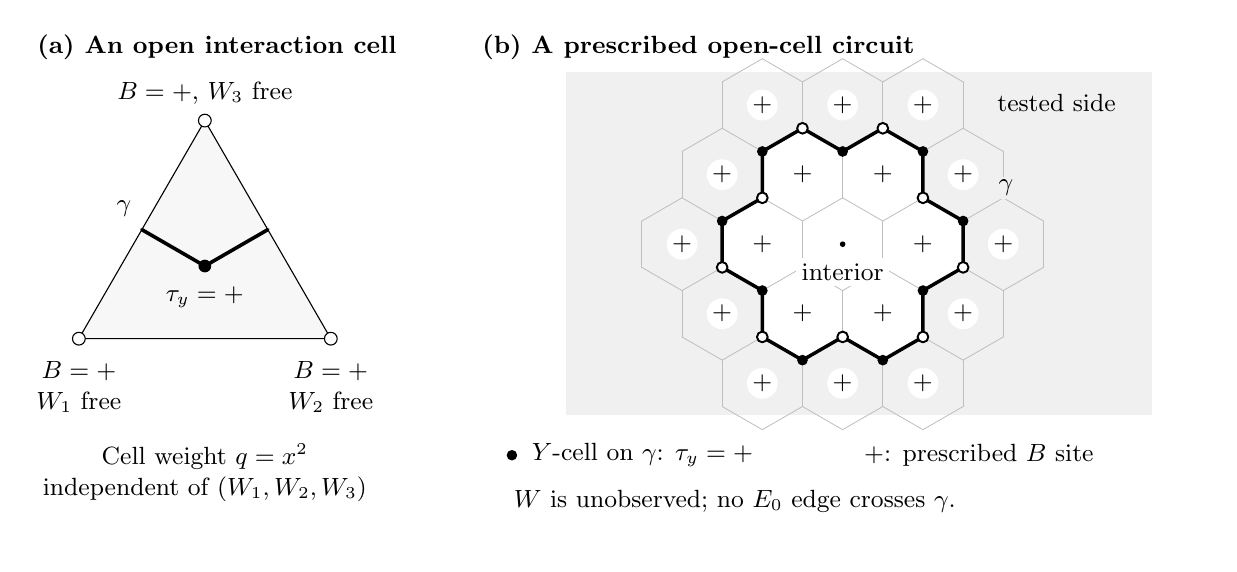
\begin{tikzpicture}[x=1cm,y=1cm,font=\fontsize{9}{11}\selectfont,
  line cap=round,line join=round]
\path[use as bounding box] (0,-1.25) rectangle (15,5.3);
\node[anchor=west,font=\fontsize{9}{11}\selectfont\bfseries] at (0,5.05)
  {(a) An open interaction cell};
\draw[thin,fill=black!3] (0.65,1.35) -- (3.85,1.35) -- (2.25,4.12) -- cycle;
\draw[line width=1.3pt] (1.45,2.735) -- (2.25,2.273) -- (3.05,2.735);
\node[anchor=south east] at (1.44,2.78) {$\gamma$};
\fill (2.25,2.273) circle (2.3pt);
\node[anchor=north] at (2.25,2.13) {$\tau_y=+$};
\foreach \a/\b in {0.65/1.35,3.85/1.35,2.25/4.12}
  \draw[fill=white] (\a,\b) circle (2.3pt);
\node[anchor=south,align=center] at (2.25,4.2) {$B=+$, $W_3$ free};
\node[anchor=north,align=center] at (0.65,1.18) {$B=+$\\$W_1$ free};
\node[anchor=north,align=center] at (3.85,1.18) {$B=+$\\$W_2$ free};
\node[align=center] at (2.25,-0.35)
  {Cell weight $q=x^2$\\independent of $(W_1,W_2,W_3)$};
\node[anchor=west,font=\fontsize{9}{11}\selectfont\bfseries] at (5.65,5.05)
  {(b) A prescribed open-cell circuit};
\begin{scope}[shift={(10.35,2.55)},scale=1.02]
\fill[black!6] (-3.45,-2.13) rectangle (3.85,2.14);
\fill[white] (-1.500000,-0.288675) -- (-1.500000,0.288675) -- (-1.000000,0.577350) -- (-1.000000,1.154701) -- (-0.500000,1.443376) -- (0.000000,1.154701) -- (0.500000,1.443376) -- (1.000000,1.154701) -- (1.000000,0.577350) -- (1.500000,0.288675) -- (1.500000,-0.288675) -- (1.000000,-0.577350) -- (1.000000,-1.154701) -- (0.500000,-1.443376) -- (0.000000,-1.154701) -- (-0.500000,-1.443376) -- (-1.000000,-1.154701) -- (-1.000000,-0.577350) -- cycle;
\draw[black!25,line width=0.3pt] (-2.500000,-0.288675) -- (-2.500000,0.288675);
\draw[black!25,line width=0.3pt] (-2.500000,-0.288675) -- (-2.000000,-0.577350);
\draw[black!25,line width=0.3pt] (-2.500000,0.288675) -- (-2.000000,0.577350);
\draw[black!25,line width=0.3pt] (-2.000000,-1.154701) -- (-2.000000,-0.577350);
\draw[black!25,line width=0.3pt] (-2.000000,-1.154701) -- (-1.500000,-1.443376);
\draw[black!25,line width=0.3pt] (-2.000000,-0.577350) -- (-1.500000,-0.288675);
\draw[black!25,line width=0.3pt] (-2.000000,0.577350) -- (-2.000000,1.154701);
\draw[black!25,line width=0.3pt] (-2.000000,0.577350) -- (-1.500000,0.288675);
\draw[black!25,line width=0.3pt] (-2.000000,1.154701) -- (-1.500000,1.443376);
\draw[black!25,line width=0.3pt] (-1.500000,-2.020726) -- (-1.500000,-1.443376);
\draw[black!25,line width=0.3pt] (-1.500000,-2.020726) -- (-1.000000,-2.309401);
\draw[black!25,line width=0.3pt] (-1.500000,-1.443376) -- (-1.000000,-1.154701);
\draw[black!25,line width=0.3pt] (-1.500000,-0.288675) -- (-1.500000,0.288675);
\draw[black!25,line width=0.3pt] (-1.500000,-0.288675) -- (-1.000000,-0.577350);
\draw[black!25,line width=0.3pt] (-1.500000,0.288675) -- (-1.000000,0.577350);
\draw[black!25,line width=0.3pt] (-1.500000,1.443376) -- (-1.500000,2.020726);
\draw[black!25,line width=0.3pt] (-1.500000,1.443376) -- (-1.000000,1.154701);
\draw[black!25,line width=0.3pt] (-1.500000,2.020726) -- (-1.000000,2.309401);
\draw[black!25,line width=0.3pt] (-1.000000,-2.309401) -- (-0.500000,-2.020726);
\draw[black!25,line width=0.3pt] (-1.000000,-1.154701) -- (-1.000000,-0.577350);
\draw[black!25,line width=0.3pt] (-1.000000,-1.154701) -- (-0.500000,-1.443376);
\draw[black!25,line width=0.3pt] (-1.000000,-0.577350) -- (-0.500000,-0.288675);
\draw[black!25,line width=0.3pt] (-1.000000,0.577350) -- (-1.000000,1.154701);
\draw[black!25,line width=0.3pt] (-1.000000,0.577350) -- (-0.500000,0.288675);
\draw[black!25,line width=0.3pt] (-1.000000,1.154701) -- (-0.500000,1.443376);
\draw[black!25,line width=0.3pt] (-1.000000,2.309401) -- (-0.500000,2.020726);
\draw[black!25,line width=0.3pt] (-0.500000,-2.020726) -- (-0.500000,-1.443376);
\draw[black!25,line width=0.3pt] (-0.500000,-2.020726) -- (0.000000,-2.309401);
\draw[black!25,line width=0.3pt] (-0.500000,-1.443376) -- (0.000000,-1.154701);
\draw[black!25,line width=0.3pt] (-0.500000,-0.288675) -- (-0.500000,0.288675);
\draw[black!25,line width=0.3pt] (-0.500000,-0.288675) -- (0.000000,-0.577350);
\draw[black!25,line width=0.3pt] (-0.500000,0.288675) -- (0.000000,0.577350);
\draw[black!25,line width=0.3pt] (-0.500000,1.443376) -- (-0.500000,2.020726);
\draw[black!25,line width=0.3pt] (-0.500000,1.443376) -- (0.000000,1.154701);
\draw[black!25,line width=0.3pt] (-0.500000,2.020726) -- (0.000000,2.309401);
\draw[black!25,line width=0.3pt] (0.000000,-2.309401) -- (0.500000,-2.020726);
\draw[black!25,line width=0.3pt] (0.000000,-1.154701) -- (0.000000,-0.577350);
\draw[black!25,line width=0.3pt] (0.000000,-1.154701) -- (0.500000,-1.443376);
\draw[black!25,line width=0.3pt] (0.000000,-0.577350) -- (0.500000,-0.288675);
\draw[black!25,line width=0.3pt] (0.000000,0.577350) -- (0.000000,1.154701);
\draw[black!25,line width=0.3pt] (0.000000,0.577350) -- (0.500000,0.288675);
\draw[black!25,line width=0.3pt] (0.000000,1.154701) -- (0.500000,1.443376);
\draw[black!25,line width=0.3pt] (0.000000,2.309401) -- (0.500000,2.020726);
\draw[black!25,line width=0.3pt] (0.500000,-2.020726) -- (0.500000,-1.443376);
\draw[black!25,line width=0.3pt] (0.500000,-2.020726) -- (1.000000,-2.309401);
\draw[black!25,line width=0.3pt] (0.500000,-1.443376) -- (1.000000,-1.154701);
\draw[black!25,line width=0.3pt] (0.500000,-0.288675) -- (0.500000,0.288675);
\draw[black!25,line width=0.3pt] (0.500000,-0.288675) -- (1.000000,-0.577350);
\draw[black!25,line width=0.3pt] (0.500000,0.288675) -- (1.000000,0.577350);
\draw[black!25,line width=0.3pt] (0.500000,1.443376) -- (0.500000,2.020726);
\draw[black!25,line width=0.3pt] (0.500000,1.443376) -- (1.000000,1.154701);
\draw[black!25,line width=0.3pt] (0.500000,2.020726) -- (1.000000,2.309401);
\draw[black!25,line width=0.3pt] (1.000000,-2.309401) -- (1.500000,-2.020726);
\draw[black!25,line width=0.3pt] (1.000000,-1.154701) -- (1.000000,-0.577350);
\draw[black!25,line width=0.3pt] (1.000000,-1.154701) -- (1.500000,-1.443376);
\draw[black!25,line width=0.3pt] (1.000000,-0.577350) -- (1.500000,-0.288675);
\draw[black!25,line width=0.3pt] (1.000000,0.577350) -- (1.000000,1.154701);
\draw[black!25,line width=0.3pt] (1.000000,0.577350) -- (1.500000,0.288675);
\draw[black!25,line width=0.3pt] (1.000000,1.154701) -- (1.500000,1.443376);
\draw[black!25,line width=0.3pt] (1.000000,2.309401) -- (1.500000,2.020726);
\draw[black!25,line width=0.3pt] (1.500000,-2.020726) -- (1.500000,-1.443376);
\draw[black!25,line width=0.3pt] (1.500000,-1.443376) -- (2.000000,-1.154701);
\draw[black!25,line width=0.3pt] (1.500000,-0.288675) -- (1.500000,0.288675);
\draw[black!25,line width=0.3pt] (1.500000,-0.288675) -- (2.000000,-0.577350);
\draw[black!25,line width=0.3pt] (1.500000,0.288675) -- (2.000000,0.577350);
\draw[black!25,line width=0.3pt] (1.500000,1.443376) -- (1.500000,2.020726);
\draw[black!25,line width=0.3pt] (1.500000,1.443376) -- (2.000000,1.154701);
\draw[black!25,line width=0.3pt] (2.000000,-1.154701) -- (2.000000,-0.577350);
\draw[black!25,line width=0.3pt] (2.000000,-0.577350) -- (2.500000,-0.288675);
\draw[black!25,line width=0.3pt] (2.000000,0.577350) -- (2.000000,1.154701);
\draw[black!25,line width=0.3pt] (2.000000,0.577350) -- (2.500000,0.288675);
\draw[black!25,line width=0.3pt] (2.500000,-0.288675) -- (2.500000,0.288675);
\draw[line width=1.25pt] (-1.500000,-0.288675) -- (-1.500000,0.288675) -- (-1.000000,0.577350) -- (-1.000000,1.154701) -- (-0.500000,1.443376) -- (0.000000,1.154701) -- (0.500000,1.443376) -- (1.000000,1.154701) -- (1.000000,0.577350) -- (1.500000,0.288675) -- (1.500000,-0.288675) -- (1.000000,-0.577350) -- (1.000000,-1.154701) -- (0.500000,-1.443376) -- (0.000000,-1.154701) -- (-0.500000,-1.443376) -- (-1.000000,-1.154701) -- (-1.000000,-0.577350) -- cycle;
\draw[fill=white,line width=0.7pt] (-1.500000,-0.288675) circle (1.9pt);
\fill (-1.500000,0.288675) circle (1.9pt);
\draw[fill=white,line width=0.7pt] (-1.000000,0.577350) circle (1.9pt);
\fill (-1.000000,1.154701) circle (1.9pt);
\draw[fill=white,line width=0.7pt] (-0.500000,1.443376) circle (1.9pt);
\fill (0.000000,1.154701) circle (1.9pt);
\draw[fill=white,line width=0.7pt] (0.500000,1.443376) circle (1.9pt);
\fill (1.000000,1.154701) circle (1.9pt);
\draw[fill=white,line width=0.7pt] (1.000000,0.577350) circle (1.9pt);
\fill (1.500000,0.288675) circle (1.9pt);
\draw[fill=white,line width=0.7pt] (1.500000,-0.288675) circle (1.9pt);
\fill (1.000000,-0.577350) circle (1.9pt);
\draw[fill=white,line width=0.7pt] (1.000000,-1.154701) circle (1.9pt);
\fill (0.500000,-1.443376) circle (1.9pt);
\draw[fill=white,line width=0.7pt] (0.000000,-1.154701) circle (1.9pt);
\fill (-0.500000,-1.443376) circle (1.9pt);
\draw[fill=white,line width=0.7pt] (-1.000000,-1.154701) circle (1.9pt);
\fill (-1.000000,-0.577350) circle (1.9pt);
\node[font=\fontsize{9}{11}\selectfont,inner sep=0.6pt,circle,fill=white] at (-2.000000,0.000000) {$+$};
\node[font=\fontsize{9}{11}\selectfont,inner sep=0.6pt,circle,fill=white] at (-1.500000,0.866025) {$+$};
\node[font=\fontsize{9}{11}\selectfont,inner sep=0.6pt,circle,fill=white] at (-1.000000,1.732051) {$+$};
\node[font=\fontsize{9}{11}\selectfont,inner sep=0.6pt,circle,fill=white] at (-1.500000,-0.866025) {$+$};
\node[font=\fontsize{9}{11}\selectfont,inner sep=0.6pt,circle,fill=white] at (-1.000000,0.000000) {$+$};
\node[font=\fontsize{9}{11}\selectfont,inner sep=0.6pt,circle,fill=white] at (-0.500000,0.866025) {$+$};
\node[font=\fontsize{9}{11}\selectfont,inner sep=0.6pt,circle,fill=white] at (0.000000,1.732051) {$+$};
\node[font=\fontsize{9}{11}\selectfont,inner sep=0.6pt,circle,fill=white] at (-1.000000,-1.732051) {$+$};
\node[font=\fontsize{9}{11}\selectfont,inner sep=0.6pt,circle,fill=white] at (-0.500000,-0.866025) {$+$};
\fill (0.000000,0.000000) circle (1pt);
\node[font=\fontsize{9}{11}\selectfont,inner sep=0.6pt,circle,fill=white] at (0.500000,0.866025) {$+$};
\node[font=\fontsize{9}{11}\selectfont,inner sep=0.6pt,circle,fill=white] at (1.000000,1.732051) {$+$};
\node[font=\fontsize{9}{11}\selectfont,inner sep=0.6pt,circle,fill=white] at (0.000000,-1.732051) {$+$};
\node[font=\fontsize{9}{11}\selectfont,inner sep=0.6pt,circle,fill=white] at (0.500000,-0.866025) {$+$};
\node[font=\fontsize{9}{11}\selectfont,inner sep=0.6pt,circle,fill=white] at (1.000000,0.000000) {$+$};
\node[font=\fontsize{9}{11}\selectfont,inner sep=0.6pt,circle,fill=white] at (1.500000,0.866025) {$+$};
\node[font=\fontsize{9}{11}\selectfont,inner sep=0.6pt,circle,fill=white] at (1.000000,-1.732051) {$+$};
\node[font=\fontsize{9}{11}\selectfont,inner sep=0.6pt,circle,fill=white] at (1.500000,-0.866025) {$+$};
\node[font=\fontsize{9}{11}\selectfont,inner sep=0.6pt,circle,fill=white] at (2.000000,0.000000) {$+$};
\node[fill=white,inner sep=2pt] at (0,-0.35) {interior};
\node[anchor=west,fill=black!6,inner sep=2pt] at (1.85,1.76) {tested side};
\node[anchor=west,fill=black!6,inner sep=1pt] at (1.9,0.7) {$\gamma$};
\end{scope}
\fill (6.15,-0.13) circle (1.9pt);
\node[anchor=west] at (6.28,-0.13) {$Y$-cell on $\gamma$: $\tau_y=+$};
\node[anchor=west] at (10.5,-0.13) {$+$: prescribed $B$ site};
\node[anchor=west] at (6.05,-0.72)
  {$W$ is unobserved; no $E_0$ edge crosses $\gamma$.};
\end{tikzpicture}

 \caption{An exact open-cell cut. In (a), prescribing $B=+$ and
 $\tau_y=+$ gives the constant cell weight $q=x^2$ for every second-spin
 assignment. In (b), filled circuit vertices are open-plus $Y$ cells;
 plus signs mark their prescribed first-spin sites. The tested exterior
 is shaded. No equality edge crosses $\gamma$, and the unobserved second
 spins have no component joining its two sides. Strictly interior cells
 retain their original interactions.}
 \label{discrete:fig-cut}
\end{figure}

\begin{samepage}
Here is the only crossing estimate imported into the discrete argument.
The boundary convention in its statement is part of the theorem.

\begin{theorem}[Glazman--Lammers circuit input]\label{thm:circuit-input}
For $r\ge0$, let $\Lambda_r$ be the ball of radius $r$ in the triangular
graph metric, with its bounding honeycomb contour; thus
$\Lambda_r=\Lambda_{\lfloor r\rfloor}$. For $a>1$ and an integer
$n\in\N$, consider on
$\Lambda_{an}$ the cell spin law whose
interior cells have weight $(x^2)^{\ind\{B\text{ or }W\text{ nonconstant}\}}$
and whose boundary $Y$ cells are excluded. Fix $B=-$ on the boundary face
layer and leave $W$ free. There is $c=c(x,a)>0$ such
that, for $n\ge 3/(a-1)$, the probability of an occupied open-plus cell
circuit surrounding $\Lambda_n$ and contained in $\Lambda_{an}$ is at
least $c$. The same statement holds with the signs or the two spin colors
interchanged.
\end{theorem}
\end{samepage}

This is equation (55) in Appendix A of the third arXiv version of
\cite{GL2025}, with Definitions 3.2 and 3.5. Its augmentation includes a
cell whenever $W$ is nonconstant, excludes it whenever $B$ is nonconstant,
and otherwise includes it with probability $x^2$. It is therefore exactly
\eqref{discrete:cell-table}. The source uses
$Y(\Omega)=(Y\cap V(\Omega))\setminus V(\partial\Omega)$; simply pinning
$B=-$ in our edge-weight law would still charge certain boundary $W$
changes. Lemma~\ref{lem:cell-cut} instead identifies the source law with
the law inside a prescribed regular open-minus circuit: the excluded
boundary factors become constants. This is also the conditional law
described by Lemma 3.8 of \cite{GL2025}. We use the theorem only through
this exact identification, with fixed slack for lattice rounding. In
particular its validity includes $x=1/\sqrt2$.

\subsection{Restricted histories and the two-law inequality}

A \emph{history} fixes some first-spin sites and some cell statuses, with
the rule that it fixes \emph{all} first-spin sites of every observed cell.
The equality set $E_0$ remains deterministic. No second-spin component
labels are part of a history. Order first spins by $-<+$ and statuses by
$-<0<+$. Ordered histories have the same observation sets and ordered
values. They may also have additional deterministic plus $B$ pins only in
the upper law, or additional deterministic minus $B$ pins only in the
lower law, compatible with the common pins.

\begin{proposition}[Association and conditional order]\label{prop:history-order}
For every feasible history, the unobserved $(B,\tau)$ variables are
positively associated. Two laws with ordered histories and common $E_0$
are stochastically ordered, including the unequal extreme pins just
described. Extra prescribed open-plus cells only in the upper law, or
open-minus cells only in the lower law, can be incorporated by observing
those cells and all their first-spin sites also in the other law. These
claims hold for clipped cells and at $x=1$.
\end{proposition}

We first prove two finite-weight inequalities used in the proof of this
proposition, then apply them to the cell law.

We use the finite association inequality of Fortuin--Kasteleyn--Ginibre
\cite{FKG1971}, including weights that vanish.  Its precise form follows
from the rounded-midpoint inequality stated and tensorized in
Theorem~\ref{thm:midpoint}: for nonnegative finitely supported arrays,
the premise
$f(b)g(c)\le u(\lfloor(b+c)/2\rfloor)v(\lceil(b+c)/2\rceil)$
implies $(\sum f)(\sum g)\le(\sum u)(\sum v)$.
Indeed, on a Boolean cube the rounded
midpoints of $b,c$ are their coordinatewise minimum $b\wedge c$ and
maximum $b\vee c$.  If a nonnegative weight $w$ satisfies
$w(b)w(c)\le w(b\wedge c)w(b\vee c)$ and $F,G$ are nonnegative
increasing functions, then
\[
 w(b)F(b)w(c)G(c)
 \le w(b\wedge c)w(b\vee c)F(b\vee c)G(b\vee c).
\]
Apply the midpoint inequality to $wF,wG,w,wFG$, extended by zero
outside the cube.  Its conclusion is
$(\sum wF)(\sum wG)\le(\sum w)(\sum wFG)$, which is association
after normalization.  Encode an element of a finite chain by a prefix
of ones followed by zeros.  The encoded product of chains is closed
under minimum and maximum, so extension by zero proves the same result
there.  Adding constants to bounded increasing functions covers signed
functions.  This deduction explains every finite association use below;
the midpoint tensorization itself uses no association statement.

The wall decomposition below expresses the first-spin weight using two
partition sums for the complementary spin.  We record the two properties
of those sums needed to compare first-spin configurations.

\begin{lemma}[The complementary-spin partition sum]
\label{discrete:ising-partition}
For $a\in[0,1]^E$ define
\begin{equation}\label{discrete:ising-Z}
 Z(a)=\sum_{\sigma\in\{-,+\}^{V}}
             \prod_{e=uv\in E}a_e^{\ind\{\sigma_u\ne\sigma_v\}},
 \qquad 0^0=1.
\end{equation}
Then $Z$ is increasing in every coordinate and is log-supermodular:
\begin{equation}\label{discrete:Z-lattice}
 Z(a\wedge b)Z(a\vee b)\ge Z(a)Z(b).
\end{equation}
\end{lemma}
\begin{proof}
Monotonicity follows term by term.  For positive coordinates the second assertion follows by differentiating in $\log a_e$.
For distinct edges $e=uv$ and $f=st$,
\[
 \frac{\partial^2\log Z}{\partial\log a_e\,\partial\log a_f}
 =\Cov(\ind\{\sigma_u\ne\sigma_v\},
              \ind\{\sigma_s\ne\sigma_t\})
 =\tfrac14\Cov(\sigma_u\sigma_v,\sigma_s\sigma_t)\ge0.
\]
The last inequality is a special case of the second Griffiths inequality
\cite{GKS1968}; we recall its random-cluster proof \cite[p.~102]{FKG1971}. Put
$J_e=-\frac12\log a_e\ge0$ and $p_e=1-e^{-2J_e}=1-a_e$. Expanding
\[
 e^{J_e\sigma_u\sigma_v}
 =e^{J_e}\bigl((1-p_e)+p_e\ind\{\sigma_u=\sigma_v\}\bigr)
\]
over edges gives a joint spin--bond law whose bond marginal on
$\omega\subset E$ has weight
\[
 2^{k(\omega)}\prod_{e\in\omega}p_e
                    \prod_{e\notin\omega}(1-p_e),
\]
where $k(\omega)$ counts all connected components, including isolated
vertices. This weight satisfies the lattice condition. Indeed, if
$\mathcal C(A)$ is the binary cycle space of the edge set $A$, then
$\mathcal C(A)\cap\mathcal C(B)=\mathcal C(A\cap B)$ and
$\mathcal C(A)+\mathcal C(B)\subset\mathcal C(A\cup B)$.
Taking dimensions and using
$k(A)=|V|-|A|+\dim\mathcal C(A)$ proves supermodularity of $k$;
the remaining edge factors are modular. The FKG theorem
\cite{FKG1971} therefore associates increasing bond events.
Conditional on $\omega$, the spins are independent fair signs on its
components. Consequently
$\E(\sigma_u\sigma_v)=\Prob(u\leftrightarrow v)$, while the
conditional expectation of $\sigma_u\sigma_v\sigma_s\sigma_t$ is
one precisely when each component contains an even number of the four
listed vertices, counted with multiplicity, and is zero otherwise. In
particular
\[
 \E(\sigma_u\sigma_v\sigma_s\sigma_t)
 \ge\Prob(u\leftrightarrow v,\ s\leftrightarrow t)
 \ge\Prob(u\leftrightarrow v)\Prob(s\leftrightarrow t).
\]
This proves the required covariance inequality, also when the edges share
vertices. The cases $p_e\in\{0,1\}$ follow by continuity. Integrating
the nonnegative mixed derivatives over coordinate rectangles gives
\eqref{discrete:Z-lattice}; continuity of the polynomial $Z$ includes its
zero-coordinate cases.

\end{proof}


\begin{proof}[Proof of Proposition~\ref{prop:history-order}]
We first sum the second spins by splitting their walls according to the
first-spin sign.  Lemma~\ref{discrete:ising-partition} will give the
two-law inequality for this marginal.  We then restore the statuses.

Fix a first-spin configuration $b$. A binary edge set is a second-spin
wall precisely when it has even intersection with every triangle boundary.
Indeed this condition makes its mod-two integral independent of the path
from a fixed anchor, since triangle boundaries generate the cycle space.
There are exactly two spin labelings for each such wall. Every allowed wall
edge has homogeneous $b$ endpoints. Split these edges according to their
common sign. A homogeneous triangle has only one sign class. A mixed
triangle has just one homogeneous edge, which its even rule forces to be
absent. Thus none of the triangle equations couples the two sign classes.
Each sign restriction of an allowed wall is itself a wall, and arbitrary
walls supported in the two allowed sign sets can be combined. This proves
factorization without an additional global compatibility condition.

For an unobserved cell let
$r_y(b)=1$ if $b$ is homogeneous there and $r_y(b)=q_y$ otherwise.
Define $a_h^+(b)$ as follows: it equals $x$ on edges of unobserved
homogeneous-plus cells, equals $1$ on observed open-plus cells, and is zero
on all other edges. Set it to zero also on $E_0$. Define $a_h^-(b)$ with
minus in place of plus. Summing the unobserved statuses and then the second
spins gives the first-spin weight
\begin{equation}\label{discrete:wall-factor}
 w_h(b)=\frac{c_h}{2}\,
   \prod_{y\text{ unobserved}}r_y(b)\,
   Z(a_h^+(b))Z(a_h^-(b))\,
   \ind\{b\text{ satisfies its fixed sites}\}.
\end{equation}
Here $c_h>0$ is the product of the observed-cell factors; these are
constants because their first spins are fixed. The factor $1/2$ is exact:
each $Z$ counts two global signs whereas the actual second-spin sum counts
only two, not four. In particular $E_0$ deletes wall coordinates and does
not impose a relation between the two global signs. Formula
\eqref{discrete:wall-factor} would in general fail on a graph with a hole
if the missing cycle constraints were omitted, explaining our ambient
triangulation convention.

Let $h_-\le h_+$ be ordered histories. For any $b$ in the lower support and
$c$ in the upper support, $b\wedge c$ belongs to the lower support and
$b\vee c$ to the upper support, also when pins occur in just one law.
On an unobserved cell, homogeneous-plus eligibility at the meet is the
intersection of the input eligibilities; at the join it contains their
union. Therefore, coordinatewise,
\begin{align*}
 a_{h_-}^+(b\wedge c)&\ge a_{h_-}^+(b)\wedge a_{h_+}^+(c),&
 a_{h_+}^+(b\vee c)&\ge a_{h_-}^+(b)\vee a_{h_+}^+(c),\\
 a_{h_-}^-(b\wedge c)&\ge a_{h_-}^-(b)\vee a_{h_+}^-(c),&
 a_{h_+}^-(b\vee c)&\ge a_{h_-}^-(b)\wedge a_{h_+}^-(c).
\end{align*}
On observed cells the plus vectors are already ordered and the minus
vectors reverse-ordered; hence the same inequalities hold there. Deleting
the common coordinates $E_0$ preserves all four inequalities.
Furthermore
\[
 r_y(b\wedge c)r_y(b\vee c)\ge r_y(b)r_y(c).
\]
To check this last assertion, comparable restrictions are unchanged by
sorting. For incomparable restrictions both inputs are mixed, whereas
each output has weight at least $q_y$. A homogeneous input is extremal
and cannot be lost. Applying monotonicity and
\eqref{discrete:Z-lattice} to each sign in
\eqref{discrete:wall-factor} now proves
\begin{equation}\label{discrete:two-law}
 w_{h_-}(b\wedge c)w_{h_+}(b\vee c)
       \ge w_{h_-}(b)w_{h_+}(c).
\end{equation}
Observed-cell constants cancel. This also proves the lattice condition
within either first-spin law.

For clarity, zero weights and unequal supports cause no invocation of an
unstated strictly positive version of Holley's criterion
\cite{Holley1974}. Extend the weights by zero to the whole first-spin cube
and put $\widetilde w(b,0)=w_{h_-}(b)$,
$\widetilde w(b,1)=w_{h_+}(b)$. The two within-layer inequalities and
\eqref{discrete:two-law} say that $\widetilde w$ satisfies the lattice
condition on the cube times $\{0,1\}$. The nonnegative-weight FKG theorem
\cite{FKG1971} applies. For increasing $f$, its positive covariance with
the last coordinate says exactly
$\E_{h_-}f(B)\le\E_{h_+}f(B)$. The same theorem gives association of
each first-spin law. This proves the needed extension to sorted supports.

It remains to restore statuses. Given $b$, each unobserved homogeneous
cell is eligible to open with its sign; mixed cells are necessarily closed.
Let $S_+$ and $S_-$ be the two open subsets of eligible cells. Wall
factorization now gives independent weights for these subsets. Apart from
constants their respective weights are
\begin{equation}\label{discrete:subset-weight}
 \prod_{y\in S_s}q_y
 \prod_{y\in I_s\setminus S_s}(1-q_y)\,
 Z\bigl(\ind\{e\text{ lies in an open cell of sign }s\}
                    \ind\{e\notin E_0\}\bigr),
\end{equation}
where $I_s$ is the eligible set and observed open cells of sign $s$ are
included as fixed allowed cells in the last factor. Different cells have
disjoint edge sets. The Bernoulli factor is modular; the $Z$ factor is
log-supermodular in the cell set by \eqref{discrete:Z-lattice}. Thus each
subset law is associated. The same two-law calculation shows stochastic
increase under enlarging $I_s$ or the fixed allowed cells: on a common
subset cube the sorted allowed-edge sets contain the coordinatewise
intersection and union, and the Bernoulli factors cancel. Ineligible cells
are held closed. The preceding nonnegative-weight argument again handles
these deterministic restrictions.

Increasing $b$ enlarges plus eligibility and shrinks minus eligibility.
Hence $S_+$ increases and $S_-$ decreases in inclusion order, exactly the
status order $-<0<+$. Association of the minus block is also association
in reverse inclusion order, since the covariance of decreasing functions
equals that of their negatives. The two blocks are independent. If $F,G$
are increasing functions of $(B,\tau)$, conditional association gives
$\E(FG\mid B)\ge\E(F\mid B)\E(G\mid B)$; the two conditional
expectations are increasing in $B$. Association of $B$ completes the
joint association claim. An ordered coupling of the first spins followed
by ordered conditional status kernels gives the two-law assertion.

If $q_y=1$, a homogeneous unobserved cell is open deterministically, and
an observed homogeneous closed cell is infeasible. All displayed
inequalities remain valid on feasible supports, either directly or by
continuity as $q_y\uparrow1$; no division by $1-q_y$ is used. Finally an
extra open-plus cell in the upper law has the maximum possible status and
first-spin values. Querying that same block in the lower law always gives
ordered values and retains its correct distribution. This is observation
in the other law, not imposition of the upper event on it. The open-minus
case is symmetric.
\end{proof}

\begin{remark}\label{discrete:not-raw-FKG}
Proposition~\ref{prop:history-order} asserts association of the joint law,
not the lattice condition for its unsummed density. Nor does it allow
observation of a closed status without its first spins. For example, on a
single triangle conditioned only to be closed, the first-spin weight is
$1-q$ on the two homogeneous configurations and $q$ on the six mixed
ones. Its pair covariance is $(1-2q)/(1+2q)<0$ when $q>1/2$.
\end{remark}

\subsection{Online exploration and buffered circuits}

We next specify the probabilistic meaning of coupled exploration. This
will matter again when the remaining interior is compared with a plane
sample independent of exterior observables.

\begin{lemma}[Conditional kernels at a joint record]\label{discrete:online}
Consider two finite-volume laws ordered as in
Proposition~\ref{prop:history-order}. There is an online exploration
coupling with the following invariant: conditional on every full joint
query record, the eventual completion in either coordinate has that
coordinate's original Gibbs conditional law given its own observed values
and deterministic constraints. The next cell, together with all its first
spins, may be chosen as any deterministic function of the joint record.
If the retained conditional problems become identical, their completions
can be sampled identically.
\end{lemma}
\begin{proof}
At a joint record $R$ let $\mu_i^R$ be the two specified own-history
conditional laws. Select a common query block $Q=Q(R)$ and couple its
marginals by an ordered kernel $\kappa_R$, available from
Proposition~\ref{prop:history-order}. For each possible pair of answers
$(a_1,a_2)$ recursively complete with the respective conditional laws
$\mu_i^R(\cdot\mid Q=a_i)$. This is a finite recursion: every nonterminal
query adds a new cell or site. At a terminal node with the same remaining
specification, use one draw from that common law. At any other terminal
node use any coupling of its two remaining laws.

Backward induction proves the marginal invariant. For a completed
observable $f$ in coordinate $1$, the expectation from the node $R$ is
\[
 \sum_{a_1,a_2}\kappa_R(a_1,a_2)
       \mu_1^R(f\mid Q=a_1)
 =\sum_{a_1}\mu_1^R(Q=a_1)\mu_1^R(f\mid Q=a_1)
 =\mu_1^R(f).
\]
The second coordinate is identical. Applying the same induction starting
at any reached node gives the assertion conditional on the whole joint
record, not merely on an individual history. Independent randomness used
to select a query can be put in the record and conditioned on first.
No conditioning of a previously sampled full-field coupling is involved.
\end{proof}

The following geometric exploration implements the lemma. In a prescribed
annular search area authorize the honeycomb edges incident to favorable
open $Y$ cells; edges outside the area may be declared unavailable. Start
from the exterior face set for an inward search, or from a connected inner
face layer for an outward search. Invade across unauthorized honeycomb
edges, querying the responsible cell and its full first-spin block in both
laws when needed. On reaching a prescribed authorized circuit with
clearance the invasion cannot cross it. The boundary of the invaded union
of honeycomb faces consists of authorized contours. Select the component
separating the start from the protected target, deleting inessential
excursions to obtain a simple circuit. In an inward search this is the
boundary around the component containing the connected target; in an
outward search it is the outer boundary of the invaded set.

There is no hidden revelation on the retained side. A queried cell touches
the invaded face set. A honeycomb vertex strictly on one side of an edge
contour touches only faces on that side. A queried cell meeting both sides
therefore lies on the contour and is favorable open, so its retained
first-spin sites have the prescribed contour sign. If a queried cell is
not favorable, invasion crosses all its incident unauthorized edges; it
cannot leave an unprescribed first-spin neighbor behind that cell. Thus
the only retained sites queried are prescribed cut-layer first spins.
Second-spin labels remain unqueried. In the absence of crossing $E_0$
edges, Lemma~\ref{lem:cell-cut} identifies the stopped retained law.
Together with Lemma~\ref{discrete:online}, this proves the exact stopped-cut
and common-sampling assertions for either direction of exploration.

\begin{lemma}[Buffered circuits and paths]\label{lem:buffer-circuits}
Fix a finite collection of annuli and tubes in a bounded planar region,
each with a positive-width buffer and with prescribed geometric clearance.
At mesh $\delta$, suppose the buffers contain no equality edge $E_0$ and
no first-spin pin adverse to a requested sign. Then each request for good
circuits, or connected good paths formed from a finite annular chain, has
probability bounded below by a positive constant independent of $\delta$
for all sufficiently small $\delta$. The bound is uniform over feasible
histories supported away from the buffers and over lattice translations
preserving the clearances. Requests with the same sign may be combined by
association; requests of different signs in disjoint buffers may be made
successively. In an annular stack of fixed-ratio, separated slots between
lattice scales $r$ and $L$, the probability of finding no requested good
circuit is at most
\begin{equation}\label{discrete:stack}
 C(r/L)^\alpha,
\end{equation}
for constants $C,\alpha>0$.

Moreover, conditioning a free ambient law on any deterministic collection
of open-plus cells and their first-spin values increases every increasing
event in $(B,\tau)$. This applies to a favorable path event in the ambient
plane even when its path leaves the interior of a prescribed good contour.
\end{lemma}
\begin{proof}
The primitive comparison takes place in a small \emph{filled} regular
disk whose entire larger comparison cut and interior fit inside the
buffer. In that disk consider a smaller regular annulus. Delete
favorable pins in the filled disk, which
can only decrease the probability of the favorable increasing event.
Prescribing the outer cut open with the adverse sign decreases it again
by Proposition~\ref{prop:history-order}. There are no other constraints
inside this small outer cut. Lemma~\ref{lem:cell-cut} and
Theorem~\ref{thm:circuit-input} give a positive lower bound in the
resulting deterministic regular problem. The same comparison applies
after any allowed outside history. For a minus request reverse all first
spins and the status order.

For gluing, use regular annuli of inner radius $\rho$ and outer radius
$2\rho$, with a small fixed geometric slack. Consecutive centers are
separated by a distance strictly between $\rho$ and $2\rho$ in the
triangular graph norm. Their inner balls intersect, and each inner ball
has a point outside the other's outer ball. Any two corresponding
surrounding circuits must therefore intersect: disjoint Jordan curves
with overlapping interiors would be nested, contradicting the latter
property. Intersecting good honeycomb paths of the same sign join.
Finitely many such annuli give a connected path following a prescribed
tube. A closed chain following a polygonal Jordan curve gives a closed
walk with the same winding number about its protected target, and hence
a surrounding simple circuit. Choose the annuli small enough that their
larger filled comparison disks stay in the buffer. Thus the target
annulus may enclose arbitrary pins in its hole: none lies in these small
comparison disks. Association multiplies their
fixed positive probabilities. A general fixed collar is covered by a
finite such chain. Rounding moves paths by only $O(\delta)$.

For requests in disjoint buffers expose the previous successful
constructions only in those buffers and condition on their full allowed
histories. The next buffer still has the same uniform bound, regardless
of the previous sign. For a stack choose $k\ge c_1\log(L/r)-c_2$
separated slots. Conditional on all previously inspected slots, failure
in the next slot has probability at most $1-c_3$. Thus the total failure
probability is at most $(1-c_3)^k$, which is
\eqref{discrete:stack}. Slots of bounded lattice size are absorbed into
$C$; no estimate at a sublattice scale is asserted.

Finally a prescription of open-plus cells is an extreme upper constraint.
Proposition~\ref{prop:history-order} shows that it increases every
increasing ambient event. This conclusion does not require the event to
lie inside the prescribed contour. If an ambient favorable path runs
from that contour to an interior target, the segment after its last
intersection with the contour lies inside and connects its prescribed
first-spin layer to the target. This observation requires no regularity
or interior corridor for the contour itself.
\end{proof}

\begin{proposition}[Local matching and the free plane law]\label{prop:local-mixing}
There are $C,\alpha>0$ with the following property. Suppose a finite
ambient graph contains a ball of radius $L$ together with its interaction
cells, and its law has first-spin pins and second-spin equalities, none
in that ball. Then its
pair marginal in the concentric radius-$r$ ball is within
$C(r/L)^\alpha$ in total variation of a common free plane law, for
$L\ge Cr\ge C$. The same is true with the statuses of either fixed
choice of first color. The plane law is the local limit of free ambient
laws along every exhaustion, and its unaugmented pair and increment
laws preserve translations, lattice symmetries, and height symmetries.

Adding extreme first-spin pins in a bounded inner region can be coupled
to the original law so that the configurations agree beyond a common
circuit of the added sign. If there are $k$ separated favorable annular
slots outside all the changes and no adverse pins or equality edges in
their buffers, the failure probability is at most $Ce^{-ck}$.
All matches preserve the individual conditional marginals at every joint
record as in Lemma~\ref{discrete:online}.
\end{proposition}
\begin{proof}
Inside the pin-free radius-$L$ ball choose a deterministic regular
open-minus cut of radius comparable to $L$. Let $\mu^-$ be the original
law with this extra prescription. It is below the original law $\mu$.
Query the cut cells also in $\mu$, and use the ordered online kernels
thereafter. Search inward in separated annular slots for a good plus
circuit in the lower law. By Lemma~\ref{lem:buffer-circuits}, the failure
probability is $C(r/L)^\alpha$. A plus cell in the lower law is plus also
in the upper law, so the selected circuit is common. The exploration
geometry just proved leaves identical inner conditional problems, with
no equality edges or pins. Sample them once, including their free
second-spin component labels. The inside law of the deterministic minus
cut is independent of all the original exterior constraints. Thus every
eligible $\mu$ is within $C(r/L)^\alpha$ of this common comparison law
on the small ball.

For two free ambient volumes containing a radius-$L$ ball this gives a
total-variation distance at most $2C(r/L)^\alpha$ on the radius-$r$ ball.
The finite-state local marginals are Cauchy along any exhaustion. Their
consistent limits define a plane law. Comparing any given finite ambient
law first with a much larger free volume and then taking its limit gives
the claimed bound, with a changed constant. Apply the same argument to
translated, reflected, rotated, or spin-rotated exhaustions to obtain the
stated invariances. The augmentation itself singles out one partite
class, so only its corresponding lattice symmetries are asserted; the
unaugmented interaction \eqref{discrete:pair-weight} has all lattice
symmetries.

For additional plus pins search outward for a good plus circuit in the
lower law; every such circuit is common. On its exterior the deterministic
constraints agree and the stopped specifications are identical. The
upper law can therefore use the same exterior sample. For additional
minus pins reverse the order and the signs. The slot bound gives
$Ce^{-ck}$. The correctness of all marginal conditionings follows from
the finite recursion of Lemma~\ref{discrete:online}, followed only then by
volume limits.
\end{proof}

Two consequences of this formulation will be useful. First, every feasible
finite event consisting of first-spin pins and finitely many connected
second-spin plus constraints has positive plane probability. Find an
exterior-searched good circuit around its entire support, an event of
positive probability. In the finite inside law, make the second spin
constant plus and prescribe the desired first spins; every such first-spin
configuration has positive total weight. The finite conditional
probability is positive. Second, all finite conditional identities pass
to the plane by exhaustion, since the event being conditioned on has
positive probability. In particular height interiors with fixed traces
have the Gibbs property in the plane construction.

The next conditional form will let us match a local increment field with
a plane copy independent of distant absolute-height observations.  Its
hypothesis concerns the retained law after an exact cut; arbitrary exterior
spin labels without such a cut are not a conditioning class in
Proposition~\ref{prop:local-mixing}.

\begin{corollary}[Plane matching after a stopped cut]
\label{cor:conditional-plane-matching}
Let $\mathcal R$ be an exterior record, and let $G$ be its
successful-search event, determined by that record.  Suppose that on every successful record a good
circuit surrounds $B(z,L)$ together with its interaction cells, and that
conditional on this record the retained law is the open-cut law of
Lemma~\ref{lem:cell-cut}, with no additional inside pins or equality edges.
For $L\ge Cr\ge C$, the pair variables in $B(z,r)$ can be coupled with
variables $P_r$ of the fixed free-plane marginal $\nu_r$ so that
\[
 \Prob(P_r\in A\mid\mathcal R)=\nu_r(A)
 \quad\text{for every event }A,
 \qquad
 \Prob(\text{mismatch}\mid\mathcal R)\le C(r/L)^\alpha
 \quad\text{on }G.
\]
The same plane marginal is assigned on failure.  Consequently $P_r$ is
independent of the entire record and the total mismatch probability is at
most $\Prob(G^c)+C(r/L)^\alpha$.  Agreement of pair variables also matches
increments along paths contained in $B(z,r)$.
\end{corollary}
\begin{proof}
The local comparison proof applies uniformly to the retained open-cut law.
To see this directly, put a deterministic regular open-minus circuit inside
$B(z,L)$ at a radius comparable to $L$.  Adding this prescription lowers
the first-color/status law by Proposition~\ref{prop:history-order}.
The old boundary prescriptions are outside this regular circuit.  Search
inward for a common open-plus circuit and use the same annular stack and
exact inside sampling as in Proposition~\ref{prop:local-mixing}.  The error
is $C(r/L)^\alpha$, independently of the old circuit and its exterior
record.  The law inside the deterministic minus circuit is independent of
that record.  Comparing it with the free-plane law gives the stated
conditional total-variation bound, with a changed constant.

For each record choose a maximal coupling of its retained marginal with
the same second marginal $\nu_r$.  On failed records use that second
marginal and any coupling.  On these finite local state spaces the usual
maximal-coupling formula gives a measurable kernel.  The conditional
second-marginal identity in the statement proves independence from
$\mathcal R$, and averaging the mismatch bound proves the final estimate.

For a stopped exploration from Lemma~\ref{discrete:online}, assume there
are no additional pins or equality edges inside the cut and no equality
edge crosses it.  The geometric invasion above records only the prescribed first-color cut layer on the
retained side.  Exterior second-spin labels, including those needed to
read absolute heights along exterior paths, reveal no retained component
label: open crossing cells have constant factors and no equality edge
crosses the cut.  Lemma~\ref{lem:cell-cut} therefore verifies the retained-law
hypothesis for precisely these records.  Retained second-spin labels must
remain unobserved.
\end{proof}

If a connected fixed skeleton has constant $W$ by equality edges, giving
its component the actual label plus has conditional probability exactly
$1/2$, independent of $(B,\tau)$. Thus it does not bias any first-spin
search. More generally, at most $m$ connected all-plus constraints have
conditional probability between $2^{-m}$ and $1$; any failed-search
probability increases by at most $2^m$ after imposing them. Once a stopped
open cut separates all these constraints from a retained region containing
no other pins or equality edges, revealing their labels fixes no retained
component. Its conditional law
is the unlabelled open-cut law. Applying Corollary~\ref{cor:conditional-plane-matching}
inside a cut at an intermediate scale gives local plane
matching also in this situation, with constants depending on $m$ and,
if necessary, a smaller positive exponent. For example a cut between
$\sqrt{rL}$ and a fixed fraction of $L$ has failure
$C_m(r/L)^{\alpha/2}$ and leaves an inside comparison error of the same
order. Absolute exterior heights may be included in the record by
revealing paths from their sites to an exterior anchor; the inner
complementary labels remain unqueried. Zero-total interior tests do not depend on the unspecified lift offset.

\subsection{Multiplicative comparison for rare pins}

Additive mixing does not control an event whose probability tends to zero
with the mesh. We next prove the comparison that will be used for such
events. All geometric neighborhoods in this proposition are fixed before
letting $\delta$ tend to zero.

\begin{proposition}[Separated rare pins]\label{prop:rare-pins}
Fix $k$ bounded filled simply connected neighborhoods $U_1,\ldots,U_k$
with disjoint closures. In each $U_i$ let $P_i$ prescribe arbitrary first
spins on a finite site set and prescribe second-spin plus on at most
$m_i$ connected lattice subgraphs, singletons allowed. Assume the
supports stay a fixed positive distance from $\partial U_i$, so that
isolating circuit collars fit inside $U_i$, and let $m=\sum_i m_i$ be
fixed. In the free plane law,
\begin{equation}\label{discrete:rare-pins}
 c\prod_{i=1}^k\Prob(P_i)
 \le \Prob\Bigl(\bigcap_{i=1}^kP_i\Bigr)
 \le C\prod_{i=1}^k\Prob(P_i).
\end{equation}
The constants depend on $x$, $k$, $m$, and the fixed buffers, but not on
the numbers of pinned sites, the lengths of the connected subgraphs, or
lattice translations preserving the buffers. The comparison also holds
in finite free ambient volumes containing all the required comparison
collars. Previous pins inside the currently considered obstacle are
retained in both comparison laws.
\end{proposition}
\begin{proof}
We first establish a single-sign comparison under arbitrary existing
first-spin pins and second-spin equalities. Consider an obstacle $K$
with an empty collar, and an event $A$ adding only first-spin pins of
sign $s$ on $K$. There can be previous pins of either sign inside $K$,
as well as equality edges there. Choose a deterministic outer good cut
$\gamma_s$ of sign $s$ in the collar. Let $p_*$ be the probability of
$A$ in the law with this additional cut. By the exact-cut lemma, $p_*$
depends on the previous \emph{inside} constraints and on the chosen
outer cut, but not on any remote constraints. Order gives
\begin{equation}\label{discrete:pstar}
 \Prob(A)\le p_*.
\end{equation}
For minus pins this is the same assertion in reversed order.

An exterior search finds a closer good cut $C_s$ of sign $s$ in a
strictly inner collar with probability at least $c_0>0$, uniformly over
all existing constraints. Conditional on any stopped successful record,
the remaining conditional probability of $A$ is exactly its probability
inside $C_s$, with all previous internal constraints retained. In the
deterministic outer-cut law, conditioning on this particular closer
favorable cut increases the event $A$. Its inside law is the same by
Lemma~\ref{lem:cell-cut}; hence the conditional probability is at least
$p_*$. Averaging over successful records proves
\begin{equation}\label{discrete:single-sign}
 c_0p_*\le\Prob(A)\le p_*.
\end{equation}
In particular probabilities under two different remote constraint sets
are comparable whenever their previous internal constraints coincide.
This argument retains opposite pins inside the obstacle; it does not
erase them when the next sign block is considered.

Write $E_i$ for the event that each of the specified second-spin
subgraphs in obstacle $i$ is constant, and $L_i$ for the event that their
labels are all plus. Initially impose no first-spin pins. Apply
\eqref{discrete:single-sign} with $W$ as first color to the events $L_i$,
obstacle by obstacle. Each conditional factor, given earlier obstacles,
is comparable with its unconditional factor, because those constraints
are remote and the same reference cut can be used. Therefore
\[
 \Prob\Bigl(\bigcap_i L_i\Bigr)\asymp\prod_i\Prob(L_i).
\]
The component-label estimate gives, both jointly and separately,
\[
 2^{-m}\Prob\Bigl(\bigcap_i E_i\Bigr)
 \le\Prob\Bigl(\bigcap_i L_i\Bigr)
 \le\Prob\Bigl(\bigcap_i E_i\Bigr),\qquad
 2^{-m_i}\Prob(E_i)\le\Prob(L_i)\le\Prob(E_i).
\]
Consequently $\Prob(\bigcap_iE_i)\asymp\prod_i\Prob(E_i)$.

Now regard all $E_i$ as the common equality set $E_0$ for the original
first color. Let $A_i$ be its prescribed first-spin event. Add the plus
pins in obstacle $1$, then its minus pins, then the two blocks in obstacle
$2$, and so on. At each step \eqref{discrete:single-sign} compares the
conditional probability with the same factor in the individual law
conditioned on $E_i$ and on earlier sign blocks \emph{in this obstacle}.
Remote $E_j$ and earlier remote first-spin pins disappear behind the
reference cut. Previous internal plus pins remain when the minus block
is added. There are at most $2k$ factors, so multiplication gives
\[
 \Prob\Bigl(\bigcap_i A_i\,\Bigm|\,\bigcap_i E_i\Bigr)
       \asymp\prod_i\Prob(A_i\mid E_i).
\]
Combining with the equality comparison gives
$\Prob(\bigcap_i(A_i\cap E_i))\asymp
\prod_i\Prob(A_i\cap E_i)$. Finally restoring all the actual plus
labels costs a factor between $2^{-m}$ and $1$, even after the arbitrary
first-spin pins and statuses have been specified. The same holds
individually with $m_i$. Since $P_i=A_i\cap L_i$, this proves
\eqref{discrete:rare-pins}. Every comparison was finite-volume and
uniform. Positive probability of the finite pin events permits passage
to the plane limit. No division by a mesh-dependent lower bound for a
pin probability occurred.
\end{proof}

\subsection{Protected switches and height order}

A spin configuration records height only modulo four.  The next switch
changes an integer lift by four in a protected region while preserving
both of its spins.  It will supply nonzero height fluctuations and allow
the moment argument to compare different integer-offset parity classes.

\begin{lemma}[Protected component switch]\label{lem:collar-switch}
Suppose two nested good circuits have opposite first-spin signs. Between
and on the two circuits assume there are no second-spin equality
constraints or prescribed second-spin labels. Conditional on the
first spins and cell statuses, there is a deterministically selectable
second-spin component in that collar whose fair label flip changes the
integer lift throughout the protected inner region by $+4$ or $-4$
relative to the protected exterior, while preserving both spins in both
protected regions. The selection uses only the first spins, statuses,
equality edges, and the two circuits. It therefore preserves any stopped
selection of the circuits based on these data.

For disjoint collars the switches commute and give equally weighted
orbits containing every parity vector of the corresponding inner lift
offsets in $4\Z$. Spin constraints and comparisons of lifts along paths
inside the protected regions are preserved. With the height anchor fixed
in the protected exterior, a test supported there is unchanged; a
zero-total test supported entirely in the protected inner region is also
unchanged. Opposite good cuts can be required in any
fixed nested pin-free collars with uniformly positive probability.
The assertion holds with the two colors interchanged.
\end{lemma}
\begin{proof}
For an oriented edge, direct use of \eqref{discrete:increment} gives
\begin{equation}\label{discrete:switch-differential}
 d(H+BW/2)=W\,dB.
\end{equation}
Whenever $B$ changes, $W$ is constant on that edge and its endpoints
belong to the same closed-cell component. For such a component $C$ define
an edge form $\omega_C$ equal to $dB$ on its changing edges and zero on
the other edges. On any triangle the two changing edges, if present,
share a vertex and consequently belong to the same component. Their
contributions cancel. Thus $\omega_C$ has zero circulation and, by simple
connectedness, has a potential $\psi_C$.

On $C$ one has $\psi_C=B+\text{constant}$, since this is true along each
closed-cell or equality edge of a component path. Every site outside $C$
can be joined to a first site of $C$ by a path whose preceding edges have
zero $\omega_C$. A changing last edge would put both endpoints in $C$,
so it too has zero form. Hence every value of $\psi_C$ is a value attained
on $C$, and its range has diameter at most two. In particular its
nonzero differences are $\pm2$.

Open cuts prevent these components from crossing either circuit. Choose
a path in the collar from the exterior-side layer of the inner circuit
to the interior-side layer of the outer circuit. The difference of its
first-spin endpoints is $\pm2$. Since
$\sum_Cd\psi_C=dB$, at least one component meeting this path contributes
a difference $\pm2$. Such a component is confined to the collar; its
potential is constant on each connected protected inner and outer
region. Choose the first such component in a fixed deterministic order.
No label of this component is prescribed. Let its label be $w\in\{-,+\}$.
Flipping it changes the right side of
\eqref{discrete:switch-differential} by $-2w\,d\psi_C$. Neither endpoint
spin changes in the protected regions, so their relative height shift is
$-2w(\pm2)=\pm4$. Anchor the lift in the protected exterior to fix its
absolute value there. The flip is an involution preserving its
conditional probability because the label is fair.

The chosen component and circuits are unchanged by this operation,
since they depend only on $(B,\tau,E_0)$. A switch changes an inner
offset $4t$ to $4(t\pm1)$ and therefore reverses its parity. Switches in
disjoint collars act on disjoint components and commute. Every orbit
has $2^j$ equally weighted elements for $j$ collars and visits each
parity vector exactly once. This conclusion remains true after imposing
any checks invariant under the switches; it asserts an orbit identity,
not independence after arbitrary checks. The statements about tests
follow from their supports and total weights. If a central event involves
absolute offsets and is not invariant, one must enlarge its bounded
range to contain the orbit before applying this identity. Finally apply
Lemma~\ref{lem:buffer-circuits} successively in two disjoint nested
collars to require opposite signs, with the given constraints away from
both buffers. Swapping the colors is a symmetry of the Gray representation.
\end{proof}

\begin{lemma}[Height comparison and flat loops]\label{lem:height-order}
Let the free sites be in bounded faces of a connected triangular-lattice
skeleton of fixed integer trace. Include all neighbors of free sites up
to that trace. The weighted height law is positively associated, and
ordered feasible traces give stochastically ordered laws. The assertion
also applies after restricting to components separated by further fixed
curves. With constant trace, the changing dual edges are disjoint closed
honeycomb loops. Given their unoriented geometry their jumps are
independent fair signs. Exposing such loops from the outside leaves in
each unexposed interior the empty-exterior loop law with the appropriate
constant inner boundary layer.
\end{lemma}
\begin{proof}
Write the edge potential as
\[
 V(t)=\begin{cases}-(\log x)|t|,&t\in\{-1,0,1\},\\
                    +\infty,&\text{otherwise}.
       \end{cases}
\]
This is a convex extended-real potential on the integers. For two
admissible arrays $h,g$, sorting their endpoint values gives on each edge
\[
 V((h\wedge g)_v-(h\wedge g)_u)
 +V((h\vee g)_v-(h\vee g)_u)
 \le V(h_v-h_u)+V(g_v-g_u).
\]
For completeness, if the endpoint orders agree this is equality. If
they disagree, write the four ordered endpoint values; sorting replaces
two crossing intervals by two nested pairings and cannot increase the
sum of their lengths. The new edge differences lie between the two old
ones, so their absolute values remain at most one. Since $-\log x\ge0$,
the displayed inequality follows, including $x=1$. Ordered traces put
the meet in the lower support and the join in the upper support.
Multiplying the edge inequalities proves the within-law lattice
condition and the two-law inequality. Heights are bounded in this finite
problem by the trace bounds plus graph distance to the trace. FKG and
the product-with-$\{0,1\}$ argument used in
Proposition~\ref{prop:history-order} therefore give association and
ordered comparison on a finite lattice, with inadmissible arrays assigned
zero weight.

On each triangle integer Lipschitz heights take at most two consecutive
values. Its dual honeycomb vertex consequently has either zero or two
changing edges. Constant trace prevents such edges from ending on the
bounding skeleton. They thus form mutually vertex-disjoint loops. A
loop lying in a bounded face of the connected skeleton cannot enclose
any piece of that skeleton: a connection from that piece to the bounding
skeleton would cross the loop. Every choice of one of two jump signs
for each loop therefore yields exactly one admissible height field with
the specified constant trace. Its weight is $x$ to the total loop length,
independent of all the signs. Conditional jumps are independent and fair,
and the marginal geometric weight is $2$ per loop times $x$ per occupied
edge.

For a fixed exposed loop, the loops strictly inside cannot touch its
vertices. The edge and loop factors split between inside and outside;
the inside boundary face layer has a constant height. Selecting the next
enclosing loop by an exploration depending only on already exposed
outside geometry does not inspect a strict inside edge. Summing the
product weights over completions, or equivalently conditioning the
constant inner height layer, proves the same factorization at each
stopping step. This is the asserted empty-exterior law and applies
without regularity of the exposed loop. Finally the ambient realization
in Lemma~\ref{lem:spin-lift}, with constant pair pins on the connected
skeleton, gives the same flat height problems used above.
\end{proof}

Every use of a positive-width buffer in later sections has the following
order of quantifiers: first fix the finite geometry, its clearances, and
its number of requests; next let $\delta\downarrow0$; only afterwards
shrink a gap or exceptional window. The constants of this section may
depend on that fixed geometry and on the fixed parameter $x$. No
uniformity as $x$ varies or as a buffer degenerates is asserted.

\section{Shell counts and smearing moments}\label{sec:moments}

All distances in this section are in lattice units.  A \emph{smearing of
radius $a\geq1$ and weight bound $A$} is a linear statistic
\begin{equation}\label{moments:weights}
 Y(H)=\sum_u w_uH(u),\qquad
 \supp w\subset B(z_0,a),\qquad
 \sum_u|w_u|\leq A,\qquad \sup_u|w_u|\leq Aa^{-2}.
\end{equation}
The weights are real and may have either sign.  If $\sum_uw_u=0$, we
call the smearing \emph{zero-total}; its value is independent of the
additive constant in the height lift.  Constants throughout may depend
on the fixed parameter $x$.

The bounded height problems below use the convention of
Lemma~\ref{lem:height-order}: a connected fixed-trace lattice skeleton
bounds the free sites, and every incident interaction up to that trace
is retained.  This includes the interior of a stopped contour after its
inner face layer has been fixed.  The skeleton need not be convex or
have a lower bound on the widths of its fjords.

We will prove two bounds for these smearings, for every finite $p\geq1$.
Suppose the radius $a$ is at most a fixed small fraction of the distance
$n$ from the smearing center to the trace.  If that trace has magnitude
at most $K$, the $L^p$ norm is controlled by
$1+K+\sqrt{\log(n/a)}$.  For zero-total smearings in the free plane
law, the norms are bounded independently of $a$.  The common starting point is a bound on the
number of enclosing loops in each shell.  It gives a logarithmic
covariance estimate and hence positive mass in a central interval;
rounded midpoints then turn that central mass into all finite moments.

\subsection{A shell estimate without an upper crossing input}

\begin{lemma}[Geometric tails for shell counts]\label{lem:shell-moments}
In a finite constant-boundary height problem, let $N_d(z)$ be the number
of level loops surrounding a site $z$ whose Euclidean closest approach
to $z$ belongs to $[d,2d)$, where $d\geq1$.  There are $c,C>0$ such that
\begin{equation}\label{moments:shell-tail}
 \Prob\{N_d(z)\geq t\}\leq Ce^{-ct}\qquad(t\geq0).
\end{equation}
In particular, for each finite $p\geq1$, $\E N_d(z)^p\leq C_p$.
These constants are independent of the shape, $z$, and $d$, and the
same assertions hold in any bounded face of a connected flat skeleton.
\end{lemma}

\begin{proof}
A constant shift reduces to boundary height zero.  Conditional on their
unoriented geometry, the level loops have independent fair height
increments.  Expose enclosing loops from outside inward, using the
stopping rule in Lemma~\ref{lem:height-order}.  If the first loop counted
by $N_d(z)$ exists, its unexplored interior has the empty-exterior loop
law with a constant inner trace.  Its distance from $z$ is at most
$2d+O(1)$.  Every further counted loop surrounds $B(z,d/2)$, for all
sufficiently large $d$.  The factor $1/2$ provides clearance from all
rounding and incident-face conventions.

We first prove a uniform obstruction in any such remaining domain.
Suppose an exterior search finds a good open-plus $B$ contour $C$ strictly
inside its boundary, surrounding $B(z,d/2)$.  Choose the outermost such
contour by the authorized-edge invasion following
Lemma~\ref{discrete:online}.  The search exposes only exterior
history and the prescribed open-plus cut data.  In particular it reveals
no strict interior cell and leaves the exact cut law of
Lemma~\ref{lem:cell-cut} inside $C$.  Moreover
\begin{equation}\label{moments:cut-radius}
 d/2\leq\dist(z,C)\leq2d+O(1).
\end{equation}
There is a number $\kappa>0$, independent of $C$, such that under this
interior law a $B$-plus path joins its prescribed inner layer to
$B(z,d/2)$ with probability at least $\kappa$.

Here are geometric and conditional details of this last assertion.
Fix a sufficiently small constant $\epsilon>0$, and choose a closest
point $p$ of $C$ to $z$.  Realize the same interior law in a new free
ambient triangulation containing $B(z,10d)$, conditioned only on the
same open-plus cells and first-spin sites of $C$.  Exact cutting
justifies this replacement even for an arbitrarily nonconvex $C$.
In this ambient graph request a good plus circuit in an annulus about
$p$ with radii $\epsilon d$ and $2\epsilon d$.  Since $C$ visits the
inner ball and surrounds $B(z,d/2)$, it must exit the outer ball and
intersect this circuit.  Next request a chain of annular plus circuits
of these same radii, from $p$ to an annulus wholly inside $B(z,d/2)$.
The centers may follow a straight segment in the ambient plane.  Choose
successive spacings strictly between $\epsilon d$ and $2\epsilon d$,
with fixed slack.  The inner balls of consecutive annuli overlap and
each protrudes outside the other's outer ball.  Consequently their
surrounding circuits intersect: disjoint circuits would have either
disjoint interiors, contradicting the overlap, or nested interiors,
contradicting that protrusion.  Equation~\eqref{moments:cut-radius}
bounds the number of requests by a constant depending only on
$\epsilon$.  Bounded lattice displacements are absorbed by the slack.

Lemma~\ref{lem:buffer-circuits} and positive association give a fixed
positive probability for their intersection in the free ambient law.
All the data imposed on $C$ are favorable for this increasing event,
so Proposition~\ref{prop:history-order} gives the same lower bound after
conditioning on $C$.  The connected circuit chain contains a path
from $C$ to the terminal circuit inside the disk.  Take its last
intersection with $C$ before that endpoint.  The remaining path stays
inside $C$, since otherwise planar separation would force another
intersection.  Its adjacent plus face chain therefore joins the
prescribed inner layer to the disk.  This proves the asserted lower
bound $\kappa$.  In particular this connection precludes a deeper
$B$ wall surrounding the disk.  The ambient chain was allowed to leave
$C$; no interior corridor of prescribed width was assumed.

To turn this obstruction into a bound on the number of loops, let $N$
be the number of further qualifying enclosing loops in the remaining
flat problem.  Closest approach is nonincreasing under nesting, so the
qualifying loops are consecutive in the enclosing nesting order until
their closest approach falls below $d$.  Conditional on all unoriented
geometry, write the height residues along them as a nearest-neighbor
walk on $\Z/4\Z$, with independent fair signs.  From every starting
residue there is a prescribed block of four signs that contains a
$W$ wall with unchanged $B=+$, followed inward by a $B$ wall.  For
example, starting from residues $0,1,2,3$, respectively, the initial
strings $++$, $--$, $---$, $+++$ have that property; complete each to
four signs arbitrarily.  Every chosen four-sign block has probability
$1/16$.  Hence, on $\{N\geq k\}$, the conditional probability of
seeing this ordered pair of walls among the first $k$ loops is at least
\[
 1-\varepsilon_k,
 \qquad \varepsilon_k=(15/16)^{\lfloor k/4\rfloor}.
\]
The statement follows by conditioning successively on the starting
residue of each block; independence between block-success events is
not required.

Call this ordered-wall event $\mathcal A$.  A $W$ wall with $B=+$ is
a good open-plus contour, because every cell at which $W$ is
nonconstant is necessarily open.  Thus $\mathcal A$ implies existence
of the exterior-searched outermost plus cut above and of a $B$ wall
strictly inside it surrounding the disk.  The preceding obstruction,
conditioned on every possible stopped cut, yields
\[
 (1-\varepsilon_k)\Prob(N\geq k)
 \leq\Prob(\mathcal A)\leq1-\kappa.
\]
Choose a fixed integer $k$ with $\varepsilon_k\leq\kappa/2$ and put
$\rho=(1-\kappa)/(1-\kappa/2)<1$.  The probability of continuing for
$k$ further qualifying loops is at most $\rho$.

After exposing these $k$ loops, the last one's interior is again an
empty-exterior flat problem of exactly the same type, with closest
boundary distance at most $2d+O(1)$.  Restarting conditionally gives
\[
 \Prob\{N_d(z)\geq1+mk\}\leq\rho^m\qquad(m\geq0).
\]
This is a stopping recursion; it asserts no independence of successive
geometric shells.  It proves~\eqref{moments:shell-tail} for sufficiently
large $d$.  For bounded $d$, each counted loop visits a fixed-size ball
and the loops have disjoint honeycomb vertices, giving a deterministic
bound on their number.  Finally, integration of the exponential tail
gives every stated moment.
\end{proof}

\begin{lemma}[Common loops and the logarithmic covariance bound]
\label{moments:covariance}
Let the flat trace be zero, let $n$ be the distance from $z_0$ to its
bounding skeleton, and let $z,w\in B(z_0,a)$, where
$1\leq a\leq c_0n$ for a sufficiently small absolute $c_0$.  With
$b=\max(1,|z-w|)$,
\begin{equation}\label{moments:covariance-bound}
 0\leq\E[H(z)H(w)]
 \leq C\left(1+\log\frac{n}{b}\right).
\end{equation}
Every smearing~\eqref{moments:weights} in this ball therefore satisfies
\begin{equation}\label{moments:second-moment}
 \E Y^2\leq C A^2\left(1+\log\frac{n}{a}\right).
\end{equation}
\end{lemma}

\begin{proof}
The independent centered loop orientations give the exact identity
\begin{equation}\label{moments:common-loops}
 \E[H(z)H(w)]
 =\E\#\{\text{level loops surrounding both $z$ and $w$}\}.
\end{equation}
Fix a dyadic closest-approach shell $[d,2d)$ about $z$ with
$d\leq b/100$.  A loop surrounding both sites and entering $B(z,2d)$
must also leave a ball about $z$ of radius comparable to $b$; otherwise
it could not enclose $w$.  It supplies a wall arm across the intervening
annuli.  Along the whole loop exactly one of $B,W$ changes.  A good
circuit of that color cannot be crossed by its wall, since the circuit's
open cells have constant first spin.

Use the wall color as the first spin.  The zero-height skeleton fixes
that first spin and imposes constancy of the second spin along a
connected skeleton.  Represent the latter constancy by $E_0$ edges.
Its actual constant label costs exactly $1/2$, independent of the
first spins and statuses, and hence does not change their marginal.
All arm annuli lie away from the skeleton, since $b\leq2a+1$ and
$c_0$ is small.  The logarithmic circuit stack from
Lemma~\ref{lem:buffer-circuits}, applied for each of the two possible
wall colors, consequently gives
\begin{equation}\label{moments:arm}
 \Prob\{\text{such a common loop exists in the shell}\}
 \leq C(d/b)^\alpha.
\end{equation}
If $M_d$ counts common loops in this shell, then
$M_d\leq N_d(z)$ and $M_d=0$ outside the event in~\eqref{moments:arm}.
Cauchy--Schwarz and Lemma~\ref{lem:shell-moments} imply
\[
 \E M_d\leq (\E N_d(z)^2)^{1/2}
       \Prob(M_d>0)^{1/2}
 \leq C(d/b)^{\alpha/2}.
\]
Loops at distance below one give a deterministic bounded contribution
by disjointness.  The sum over the small dyadic scales is bounded.
Each of the
$O(1+\log(n/b))$ remaining shells contributes at most a constant.
There are no shells beyond scale $O(n)$: a nearest skeleton site is
outside every enclosing loop, so the segment from $z$ to that site
meets the loop within distance $n+a+O(1)$.  These facts and
\eqref{moments:common-loops} prove~\eqref{moments:covariance-bound}.

For completeness the average of the singularity is uniformly bounded,
including its diagonal.  Triangular-lattice balls have at most
$C(1+r)^2$ sites.  For fixed $z$, the layer-cake formula gives, when
$a>1$,
\begin{align*}
 &\sum_w |w_w|\log^+\frac{a}{\max(1,|z-w|)}\\
 &\qquad=\int_0^{\log a}
      \sum_{\max(1,|z-w|)<ae^{-t}}|w_w|\,\dd t
 \leq C A a^{-2}\int_0^{\log a}a^2e^{-2t}\,\dd t
 \leq C A.
\end{align*}
For $a=1$ the sum vanishes.  Sum
\eqref{moments:covariance-bound} against $|w_zw_w|$, separate the
constant term $\log(n/a)$, and use this bound and
$\sum|w_z|\leq A$.  This proves~\eqref{moments:second-moment}
for arbitrary signed weights.
\end{proof}

\subsection{Weighted midpoint amplification}

We use the discrete midpoint inequality of Klartag--Lehec
\cite{KlartagLehec2019} in the nonnegative-function formulation of
Gozlan--Roberto--Samson--Tetali \cite[Theorem~3]{GRST2019}.  Its
one-dimensional finite-support statement follows directly from their
entropy inequality \cite[Theorem~8, equation~(9)]{GRST2019}, including
zero weights.  We give that deduction, its coordinate induction, and
all additional hypotheses used here.

\begin{theorem}[Discrete midpoint inequality]\label{thm:midpoint}
Let $f,g,u,v:\Z^m\longrightarrow[0,\infty)$ have finite support, and
write $m_-(s,t)=\lfloor(s+t)/2\rfloor$ and
$m_+(s,t)=\lceil(s+t)/2\rceil$, with coordinatewise rounding.
If, for every $s,t\in\Z^m$,
\[
 f(s)g(t)\leq u(m_-(s,t))v(m_+(s,t)),
\]
then
\[
 \left(\sum f\right)\left(\sum g\right)
 \leq\left(\sum u\right)\left(\sum v\right).
\]
\end{theorem}

\begin{proof}
First let $m=1$.  Write $A=\sum f$ and $B=\sum g$.
If either is zero there is nothing to prove.  Otherwise let
$\nu_0=f/A$ and $\nu_1=g/B$, and couple them monotonically: take
their quantile functions at the same uniform point of $(0,1)$.
Let $\pi$ be this coupling, and let $\nu_-,\nu_+$ be its pushforwards
by the floor and ceiling midpoint maps.  The entropy theorem just
cited states
\[
 \mathcal H(\nu_-)+\mathcal H(\nu_+)
 \le\mathcal H(\nu_0)+\mathcal H(\nu_1),
 \qquad \mathcal H(\nu)=\sum_z\nu(z)\log\nu(z),
\]
for finitely supported probability measures on $\Z$, with zero terms
omitted.  Every pair charged by $\pi$ has $f(s)g(t)>0$; the
pointwise hypothesis therefore makes both corresponding output weights
positive.  All logarithms below are thus evaluated on finite positive
supports.  Integrating the logarithm of the pointwise hypothesis and
then using the entropy inequality gives
\begin{align*}
 \log A+\log B
 &\le\sum_z\nu_-(z)\log u(z)+\sum_z\nu_+(z)\log v(z)
            -\mathcal H(\nu_0)-\mathcal H(\nu_1)\\
 &\le\left(\sum_z\nu_-(z)\log u(z)-\mathcal H(\nu_-)\right)
     +\left(\sum_z\nu_+(z)\log v(z)-\mathcal H(\nu_+)\right)\\
 &\le\log\sum_z u(z)+\log\sum_z v(z).
\end{align*}
The last inequality is Jensen's inequality applied to
$\sum\nu\log(a/\nu)$ on the positive support of each probability
measure; adding any unused nonnegative weights only enlarges the sum.
Exponentiating proves the scalar statement without modifying zero
values or assuming that a positive approximation preserves its premise.

For the induction step write $s=(s',a)$ and $t=(t',b)$.  Fix $s',t'$
and apply the one-dimensional theorem in $a,b$.  For the partial sums
$F(s')=\sum_a f(s',a)$, and likewise $G,U,V$, its conclusion is
\[
 F(s')G(t')\leq
 U(m_-(s',t'))V(m_+(s',t')).
\]
The induction hypothesis in the other $m-1$ coordinates proves the
claim.  No factorization of the functions is used.  A finite array is
extended by zero to $\Z^m$; the premise must still be checked on every
pair of its nonzero input supports.
\end{proof}

\begin{lemma}[Admissibility and energy at rounded midpoints]
\label{moments:weighted-midpoints}
Let $\mathcal S$ be the integer $1$-Lipschitz arrays on a finite
connected graph, with fixed integer heights on a nonempty set of
vertices.  Set
\[
 \mathcal W(h)=\ind_{\{h\in\mathcal S\}}
       x^{\sum_{\{i,j\}}|h_i-h_j|}.
\]
Then $\mathcal S$ is finite, both rounded midpoints of $s,t\in\mathcal S$
belong to $\mathcal S$, and
\begin{equation}\label{moments:weight-midpoint}
 \mathcal W(m_-(s,t))\mathcal W(m_+(s,t))\geq \mathcal W(s)\mathcal W(t).
\end{equation}
Moreover a linear statistic with $\sum|w_i|\leq A$ obeys
\begin{equation}\label{moments:rounding}
 \left|Y(m_\pm(s,t))-\frac{Y(s)+Y(t)}2\right|\leq A/2.
\end{equation}
The same energy inequality holds with additional support constraints
whenever both outputs satisfy those constraints.
\end{lemma}

\begin{proof}
One fixed height bounds every coordinate by its graph distance from
that vertex, so the array is finite.  For an edge $ij$ put
$a=s_i-s_j$ and $b=t_i-t_j$.  If $c,d$ are its differences in the two
rounded arrays, and $\varepsilon_i$ is the parity of $s_i+t_i$, then
\[
 c=\frac{a+b-\varepsilon_i+\varepsilon_j}{2},\qquad
 d=\frac{a+b+\varepsilon_i-\varepsilon_j}{2}.
\]
Thus $c+d=a+b$, $|c-d|\leq1$, and $c,d$ are its two nearest integer
halves.  In particular $c,d\in\{-1,0,1\}$ and
\[
 |c|+|d|=|a+b|\leq|a|+|b|.
\]
Each fixed integer coordinate is preserved exactly.  Summing over edges
and using $x\leq1$ proves~\eqref{moments:weight-midpoint}, including
$x=1$.  Each rounded coordinate differs from its average by at most
$1/2$, which proves~\eqref{moments:rounding} even for signed weights.
\end{proof}

\begin{lemma}[Central mass in finitely many classes]
\label{lem:midpoint-amplification}
Let $\mu(h)=\mathcal W(h)/Z$ be a finite probability measure on integer arrays.
Partition its support into at most $J$ classes.  Suppose that two arrays
from the same class have both rounded midpoints in the full support,
with the weight inequality~\eqref{moments:weight-midpoint}.  Let $Y$ be
a linear statistic satisfying~\eqref{moments:rounding}.  If $M>0$,
$M\geq A/2$, and, for every class $\mathcal S_i$,
\begin{equation}\label{moments:class-central}
 \mu\bigl(\mathcal S_i\cap\{|Y|\leq M\}\bigr)\geq c>0,
\end{equation}
then there are $a_*>0$ and $C_p<\infty$, depending only on $J,c,p$, such
that
\begin{equation}\label{moments:amplification}
 \mu\{|Y|>tM\}\leq4e^{-a_*t}\quad(t\geq0),
 \qquad \|Y\|_{L^p(\mu)}\leq C_pM\quad(1\leq p<\infty).
\end{equation}
Outputs may belong to any class.  In particular no stability of an
individual class under midpoint rounding is required.
\end{lemma}

\begin{proof}
For integers $j\geq3$ define
\[
 I_j=[(2^j-4)M,(2^{j+1}+4)M],\qquad p_j=\mu(Y\in I_j).
\]
For $j\geq4$ choose a class carrying at least $p_j/J$ of the mass of
$I_j$, and pair its tail arrays with its central arrays from
\eqref{moments:class-central}.  Every output has its statistic in
\[
 [(2^{j-1}-7/2)M,(2^j+7/2)M]\subset I_{j-1};
\]
indeed the central average contributes at most $M/2$ and rounding at
most $A/2\leq M$.  Apply Theorem~\ref{thm:midpoint} to $\mathcal W$ restricted
to the chosen tail and central sets, and to two copies of $\mathcal W$ restricted
to $\{Y\in I_{j-1}\}$.  Dividing by $Z^2$ gives
\begin{equation}\label{moments:recursion}
 p_j\leq (J/c)p_{j-1}^2.
\end{equation}

Put $K_*=J/c\geq1$, $N=\lceil4K_*\rceil$, and $L=3+N$.
For $j\geq4$ these intervals have overlap at most two: the upper
endpoint of $I_j$ is strictly below the lower endpoint of $I_{j+2}$.
Thus $\sum_{j\geq4}p_j\leq2$, and among $j=4,\ldots,L$ there is
$j_0$ with $K_*p_{j_0}\leq1/2$.  Iteration of
\eqref{moments:recursion} yields
\[
 K_*p_{j_0+r}\leq2^{-2^r}\quad(r\geq0),
 \qquad
 p_j\leq K_*^{-1}
 \exp\{- (\log2)2^{j-L}\}\quad(j\geq L).
\]
Repeat the argument for $-Y$, with the same $L$.  If $t\geq2^L$ and
$k=\lfloor\log_2t\rfloor$, the cores
$[2^jM,2^{j+1}M]\subset I_j$ for $j\geq k$ cover the positive tail,
and their negative counterparts cover the negative tail.  Writing
$q_0=\exp\{-(\log2)2^{k-L}\}\leq1/2$, we obtain
\[
 \mu(|Y|>tM)
 \leq\frac2{K_*}\sum_{r\geq0}q_0^{2^r}
 \leq4q_0
 \leq4\exp\{- (\log2)2^{-L-1}t\}.
\]
For $0\leq t<2^L$ the last bound exceeds one.  This proves the tail
claim with $a_*=(\log2)2^{-L-1}$.  Finally
$\E|Y|^p=\int_0^\infty pt^{p-1}\mu(|Y|>t)\,\dd t$ proves the moment
claim.  This proof explicitly uses the unconditional central mass in
each class; a central bound for their union would not suffice.
\end{proof}

\subsection{Bounded traces and plane increments}

\begin{proposition}[Smearing with bounded boundary values]
\label{prop:smearing}
In a bounded height problem as specified above, suppose its fixed trace
has absolute value at most $K$.  Let $n$ be the distance from the
smearing center to the bounding sites.  For
$1\leq a\leq c_0n$ and every finite $p\geq1$,
\begin{equation}\label{moments:smearing-bound}
 \left\|\sum_uw_uH(u)\right\|_p
 \leq C_{p,A}\left(1+K+\sqrt{\log(n/a)}\right).
\end{equation}
The bound is uniform over the shape of the trace and applies in
particular to the interior of a good cut after its complete inner
height layer has been specified.
\end{proposition}

\begin{proof}
For zero trace, Lemma~\ref{moments:covariance} and Chebyshev's inequality
supply central probability at least $1/2$ with
$M=C_A(1+\sqrt{\log(n/a)})$, increased if necessary to exceed $A/2$.
Lemma~\ref{moments:weighted-midpoints} verifies all midpoint hypotheses
for the actual weighted height measure.  Apply
Lemma~\ref{lem:midpoint-amplification} with one class to prove
\eqref{moments:smearing-bound} for zero trace.

For general trace, put $K_0=\lceil K\rceil$.  Height order from
Lemma~\ref{lem:height-order} traps the law between the flat laws with
traces $-K_0$ and $K_0$.  For nonnegative weights, the corresponding
smearing laws are the zero-trace smearing shifted by
$\pm K_0\sum_uw_u$.  Both tails are therefore bounded by the
zero-trace tails with an additive displacement at most $AK_0$.
This gives~\eqref{moments:smearing-bound}.  Split arbitrary signed
weights into their positive and negative parts; each satisfies
\eqref{moments:weights}, and the triangle inequality in $L^p$ finishes
the proof.  On a cut, fix the entire actual inner trace first, so its
interior is an ordinary weighted height problem by
Lemma~\ref{lem:cell-cut}.  The same argument applies conditionally.
\end{proof}

\begin{proposition}[Uniform plane moments for zero-total smearings]
\label{prop:plane-moments}
For the infinite-volume increment law furnished by
Proposition~\ref{prop:local-mixing}, every zero-total
smearing~\eqref{moments:weights} satisfies
\begin{equation}\label{moments:plane-bound}
 \left\|\sum_uw_uH(u)\right\|_p\leq C_{p,A}
 \qquad(1\leq p<\infty).
\end{equation}
The constants are uniform in $a\geq1$ and the center.  The same estimate
holds for the increment law in a finite free simply connected
triangulation containing $B(z_0,C_0a)$, for a sufficiently large fixed
$C_0$.
\end{proposition}

\begin{proof}
Work first with the free spin pair in the finite ambient graph.
Choose a fixed large constant $L_0$ with $1/L_0<c_0/4$, and search
from outside for a good $B$ circuit in an annulus with radii
$L_0a$ and $2L_0a$.  Choose $C_0$ large enough that all search buffers
fit in the ambient graph.  Lemma~\ref{lem:buffer-circuits} gives this
stopped-cut event probability at least $c_1>0$.  Its trace is contained
in two consecutive integers.  Conditional also on the complete inner
trace, subtract the lower of these integers.  The interior is now an
ordinary height problem with trace in $\{0,1\}$, and its distance from
$z_0$ is between fixed multiples of $L_0a$.  Proposition~\ref{prop:smearing}
therefore gives a uniform conditional second-moment bound $C_A$.
The random subtraction changes no zero-total smearing.  Chebyshev's
inequality and then averaging over the search show, for some fixed
$M\geq A/2$,
\begin{equation}\label{moments:plane-central}
 \Prob(|Y|\leq M)\geq c_1/2.
\end{equation}
If the finitely many smallest lattice scales require enlarging the
annulus to accommodate rounding, use a fixed minimal annulus radius;
its ratio to $a\geq1$ remains bounded and the same constants suffice.

To amplify this central bound, use the correct finite height measure.
For any chosen anchor $o$, the four cyclic rotations of the Gray states
preserve every increment and every interaction weight, and act
transitively on the pair state at $o$.  Consequently the unconditioned
free pair has exactly the same increment law as its version with state
$(+,+)$ at $o$.  By Lemma~\ref{lem:spin-lift}, the latter is the measure
on integer $1$-Lipschitz arrays with $H(o)=0$ and density proportional
to $x^{\sum_{ij}|H(i)-H(j)|}$.  Thus $Y$ in this anchored measure has
the central bound~\eqref{moments:plane-central}.  This argument obtains
the cut central bound before fixing the anchor, and hence introduces
no extra anchor constraint into the stopped interior law.

The anchored arrays form one midpoint-admissible class by
Lemma~\ref{moments:weighted-midpoints}.  Applying
Lemma~\ref{lem:midpoint-amplification} proves~\eqref{moments:plane-bound}
in finite volume.  At fixed lattice weights, enlarge that volume.
The increment convergence from Proposition~\ref{prop:local-mixing}
and the uniform bounds pass the estimate to the plane; higher moments
also give convergence of every fixed finite moment.  All constants
above are independent of the location and radius of the smearing.
\end{proof}

\begin{lemma}[Nondegeneracy between two disks]\label{lem:nondegeneracy}
Let $U_1,U_2$ be two fixed disjoint round disks with disjoint closures,
and let $f_i\geq0$ be smooth functions supported compactly in $U_i$,
with $\int f_i=1$.  Form their exact face-area averages on the dilated
lattice geometry of scale $R$.  If $Y_R$ is the first average minus
the second, there is $c>0$ such that
\begin{equation}\label{moments:nondegeneracy}
 \E Y_R^2\geq c
\end{equation}
for all sufficiently large $R$, in the plane and in sufficiently large
finite free volumes.  The bound is uniform under translations of the
fixed arrangement.
\end{lemma}

\begin{proof}
Choose two disjoint nested annular collars around $\supp f_1$ inside
$U_1$, avoiding $\supp f_2$.  Prescribe an outer good $B$-plus cut and
an inner good $B$-minus cut.  Successive applications of
Lemma~\ref{lem:buffer-circuits} in these separated buffers give their
joint probability at least $c_2>0$, uniformly in $R$ large enough for
rounding.  Make the choices by the stopped searches following
Lemma~\ref{discrete:online}; the event and the selected cuts
depend on first spins and cell statuses, and do not prescribe any
second-spin labels.

By Lemma~\ref{lem:collar-switch}, conditional on those variables there
is a second-spin component in the intervening collar whose fair label
flip changes every height in the inner protected region by $4$ in
absolute value relative to the exterior of the outer cut.  Choose the
component measurably using a fixed ordering, and condition on all its
other labels.  The cuts, their event, and all weights of $Y_R$ are
unchanged by this flip.  Exact unit mass in the first disk and zero
weight in the collar mean that the two values of $Y_R$ differ by $4$.
A fair pair of real numbers at distance $4$ has variance $4$ and
second moment at least $4$.  Averaging over the cut event yields
$\E Y_R^2\geq4c_2$ in finite volume.  The fourth-moment bound in
Proposition~\ref{prop:plane-moments} allows passage of these second
moments to the plane.  This proves the claim.
\end{proof}

\subsection{Exact area interpolation}

Let $Q_{\delta,u}$ be the hexagonal face centered at $u\in\delta\T$.
For a bounded compactly supported test $f$, use precisely
\begin{equation}\label{moments:area-weights}
 w_{\delta,f}(u)=\int_{Q_{\delta,u}}f(z)\,\dd z,
 \qquad
 \langle h_\delta,f\rangle
 =\sum_u w_{\delta,f}(u)h_\delta(u).
\end{equation}
This identity follows from the piecewise constant extension in the
problem, including its zero extension outside the discrete domain.
For tests supported inside that domain the tessellation gives the
exact, rather than asymptotic, identities
\[
 \sum_u w_{\delta,f}(u)=\int f,
 \qquad \sum_u|w_{\delta,f}(u)|\leq\|f\|_{L^1},
 \qquad |w_{\delta,f}(u)|\leq\frac{\sqrt3}{2}\delta^2\|f\|_\infty.
\]
In the plane these hold for every compactly supported test.  A test
supported in a disk of physical radius $r$, with
$\|f\|_1\leq A$ and $\|f\|_\infty\leq Ar^{-2}$, therefore has
smearing weights at radius $a=r/\delta+O(1)$ with a constant multiple
of the same weight bound.  For any fixed physical geometry the
condition $a\geq1$ holds once the mesh is small.  Reflection in a
lattice symmetry takes each face to its reflected face, so this
interpolation is exactly equivariant under every site reflection used
below.  A zero-integral test gives a zero-total smearing at every mesh.

In particular, on a fixed compact subset of a bounded domain,
Proposition~\ref{prop:smearing} bounds a normalized radius-$r$ average
by $C_p(1+\sqrt{\log(1/r)})$, with fixed geometry and the mesh sent
to zero first.  Finite sums of such localized smearings obey the same
bounds by the triangle inequality.  If the radius is a fixed small
fraction of the distance to a bounded trace, the right side of
\eqref{moments:smearing-bound} is uniformly bounded, even as both
physical scales subsequently tend to zero.  Finally,
Proposition~\ref{prop:plane-moments} gives a uniform bound for each
fixed bounded family of zero-total smooth tests and their dilations.
These assertions use ordinary Euclidean area weights throughout.

The class hypothesis~\eqref{moments:class-central} has deliberately
not been asserted for any spin-pinned ensemble.  The parity-class
admissibility and central mass required in that setting will be proved
in Proposition~\ref{prop:pin-moments} before
Lemma~\ref{lem:midpoint-amplification} is applied there.

\section{Reflection and the plane normalization}
\label{sec:plane}

Throughout this section the law is the free plane pair obtained in
Proposition~\ref{prop:local-mixing}, with the fixed weight
$x\in[1/\sqrt2,1]$.  Only its original nearest-neighbor interaction is used
for reflection; no reflection symmetry of the auxiliary cell variables is
needed.  Write $\xi_u=H(u)-H(0)$ for its height increments.  If
$f\in C_c^\infty(\R^2)$ has integral zero, set
\[
 H_\delta(f)=\sum_{u\in\T}w_{\delta,f}(u)H(u),\qquad
 w_{\delta,f}(u)=\int_{\delta(u+V)}f(z)\dd z,
\]
where $V$ is the closed unit-mesh hexagonal face centered at zero, with
boundaries ignored in integrals.  The faces $u+V$ tile the plane.  In
particular, $\sum_u w_{\delta,f}(u)=\int f=0$, so the statistic is
independent of the additive lift.  All these finite sums are centered by
height reflection.  We will show that their covariances converge to a
positive multiple of the plane Green form, with the same constant along
every mesh sequence.  We then use this covariance to show that a Laplace
test supported strictly on one side of a reflection line has covariance
with its reflected test tending to zero.  Reflection positivity will
interpret this as a vanishing reflection seminorm, which
Section~\ref{sec:pins} will use to transfer the Laplace identity through
separated pinning conditions.

Use Euclidean coordinates, and put
\[
 e_1=(1,0),\qquad e_2=(1/2,\sqrt3/2),\qquad
 P=\frac{2\pi}{\sqrt3},\qquad
 \T^*=\{(2\pi m,P(2n-m)):m,n\in\Z\}.
\]
The reciprocal torus is $\widehat\T=\R^2/\T^*$, with characters
$u\mapsto e^{ip\cdot u}$.  Small neighborhoods of its origin always use
their Euclidean representatives.  We use
$\widehat f(p)=\int e^{-ip\cdot z}f(z)\dd z$ for the continuum Fourier
transform.

The covariance statement below is the output of the spectral argument.
Its coefficient will be fixed by a full scalar cutoff limit, after the
possible subsequential spectra have been identified.  The proof is completed
in the final subsection; the reflection-null insertion then follows from it.

\begin{proposition}[Plane covariance and normalization]
\label{prop:plane-covariance}
There is a constant $v=v(x)\in(0,\infty)$, depending only on the fixed
weight $x$, such that for every pair of real zero-integral tests
$f,g\in C_c^\infty(\R^2)$,
\begin{align}
 \lim_{\delta\downarrow0}\E[H_\delta(f)H_\delta(g)]
 &=\frac{v}{(2\pi)^2}
       \int_{\R^2}\frac{\widehat f(p)\overline{\widehat g(p)}}{|p|^2}
                  \dd p                                      \label{plane:eq:covariance}\\
 &=\frac{v}{2\pi}\iint_{\R^2\times\R^2}
          f(z)\log\frac1{|z-w|}\,g(w)\dd z\dd w.              \notag
\end{align}
The conclusion also holds for zero-integral tests converging in
$C_c^\infty$ with a common compact support.
\end{proposition}

\subsection{Reflection positivity and normal translation}

The row-conditioning proof below is the site-reflection construction
of \cite[Section~3, example~5]{FILS1978} specialized to the present edge law.
We include the normal-translation argument because positivity of that
translation, not only reflection positivity of the field, is needed
for the nonnegative Cauchy mixture.

\begin{proposition}[Positive normal transfer]
\label{prop:reflection-transfer}
Let $\ell$ be any row of lattice sites parallel to one of the three
unoriented nearest-neighbor directions, and choose one of its closed
half-planes.  The plane pair is reflection positive across $\ell$.
The assertion remains valid after adjoining any finite collection of fields
\begin{equation}
 \label{plane:eq:phases}
 Z_s(u)=U_s\exp\{is(H(u)-H(o))\},
\end{equation}
where the $U_s$ are independent unit-circle Haar variables, independent of
the pair, and $o$ is any anchor.

More precisely, let $\theta_\ell$ act on observables by spatial reflection,
and take local functions supported in the chosen half-plane, whose
height differences are evaluated along paths in that half-plane.  Then
\[
 \langle F,G\rangle_\ell
     =\E\big[\overline{\theta_\ell F}\,G\big]
\]
is a positive semidefinite Hermitian form.  In its quotient completion,
translation farther into the half-plane by the pure normal vector of
length $\sqrt3$ is a positive self-adjoint contraction $S$.  Unit
translation along the row is a commuting unitary $U$.  At mesh $\delta$
the normal step is $\sqrt3\delta$.
\end{proposition}

\begin{proof}
Take first a reflection-symmetric finite free volume, chosen so that its
intersection with the row is connected and contains the observables under
consideration.  No edge of the triangular lattice jumps across a row of
sites.  Conditional on the row spins, the two strict sides therefore have
independent, reflected-identical laws: every original edge weight belongs
to a single side together with its row boundary.  Row spins determine
relative row heights.  If phases are present, condition also on their
values at one row anchor.  On each side the other phases are determined
from those anchor phases and the increments on that side.  Their
conditional Haar law at the row anchor is independent of the spins, even
if the original anchor $o$ was elsewhere.  Consequently
\[
 \E\big[\overline{\theta_\ell F}\,F\big]
   =\E\left[\left|\E[F\mid\text{row spins and row phases}]\right|^2\right]
   \ge0.
\]
The plane limit gives the same inequality for local functions.  Ordinary
$L^2$ approximation is also allowed, since
$|\langle F,G\rangle_\ell|\le\|F\|_2\|G\|_2$.
Changing the anchor or translating the configuration multiplies each
$U_s$ by a unit complex number determined by the increments.  Conditional
Haar measure is unchanged.  This proves stationarity and all the lattice
reflection symmetries also for the augmented law.

For the operator statement take $\ell=\{y=0\}$ and the upper half-plane.
A site has coordinates $(m+n/2,n\sqrt3/2)$.  Reflections in $y=0$ and
$y=\sqrt3/2$ send its integer coordinates respectively to
$(m+n,-n)$ and $(m+n-1,2-n)$.  Thus both are site-row reflections, and their
composition gives the pure normal translation $a=(0,\sqrt3)$.
Let $T$ denote translation of observables by $a$.  Stationarity and
$\theta_\ell T=T^{-1}\theta_\ell$ imply
\[
 \langle TF,G\rangle_\ell=\langle F,TG\rangle_\ell.
\]
Furthermore $TF$ is supported above the halfway row $y=\sqrt3/2$, and
reflection of $TF$ in that row is $\theta_\ell F$.  Reflection positivity
at that row gives $\langle F,TF\rangle_\ell\ge0$.

Boundedness must be proved before taking the quotient.  Put
$a_n=\langle T^nF,T^nF\rangle_\ell^{1/2}$.  Symmetry and reflection
Cauchy--Schwarz yield
\[
 a_n^2=\langle T^{n-1}F,T^{n+1}F\rangle_\ell
       \le a_{n-1}a_{n+1}\quad(n\ge1),
 \qquad a_n\le\|F\|_2.
\]
If $a_0=0$, the first inequality gives $a_1=0$.  Otherwise an increase
$a_1>a_0$ would, by log-convexity, force geometric growth, contradicting
the second inequality.  Hence $\|TF\|_\ell\le\|F\|_\ell$.
The operator descends to the quotient and extends to a bounded symmetric
positive operator on its completion, hence to a positive self-adjoint
contraction $S$.  Tangential translation preserves the form and has an
inverse with the same property.  It therefore gives a unitary $U$;
$U,U^{-1}$ commute with $S$.  Rotation by $\pi/3$ and $2\pi/3$, and
translation of the base row, give exactly the same construction in all
three directions.
\end{proof}

\subsection{The increment spectrum and its Cauchy representation}

\begin{lemma}[Punctured spectral measure]
\label{plane:lem:spectrum}
There is a positive, locally finite measure $C$ on
$\widehat\T\setminus\{0\}$, invariant under the lattice rotations and
reflections, such that every finitely supported real array $(b_u)$ with
$\sum b_u=0$ satisfies
\begin{equation}
 \label{plane:eq:spectrum}
 \E\left|\sum_u b_uH(u)\right|^2
   =\int\left|\sum_u b_ue^{ip\cdot u}\right|^2 C(\dd p).
\end{equation}
There is no invariant random linear tilt term.  Moreover, for some
$r_0>0$ and $K<\infty$,
\begin{equation}
 \label{plane:eq:annuli}
 C\{r\le|p|\le2r\}\le K\quad(0<r<r_0),
 \qquad
 \int_{0<|p|<r_0}|p|^t C(\dd p)<\infty\quad(t>0).
\end{equation}
\end{lemma}

\begin{proof}
Let $V_u$ be ordinary unitary translation on the plane probability space.
Lemma~\ref{spectra:unitary}, applied to the two basis translations,
constructs their scalar covariance measures $\mu_{a,b}(\dd p)$ on
$\widehat\T$.  Write $P_0$ for the common invariant projection.
All increments belong to $L^2$, since
$|\xi_u|$ is bounded by the graph distance from zero to $u$.  The cocycle
identity gives
\[
 \xi_{u+v}=\xi_v+V_v\xi_u,
 \qquad (V_v-I)\xi_u=(V_u-I)\xi_v.
\]
Put $d_u(p)=e^{ip\cdot u}-1$.  The polynomial covariance identity in
Lemma~\ref{spectra:unitary} transfers the cocycle relation to the scalar
measures.  On a patch where $d_v\ne0$, it gives
$\mu_{\xi_u,\xi_w}=\overline{d_u}d_w
\mu_{\xi_v,\xi_v}/|d_v|^2$.  Division is made first on compact
subpatches where the denominator is bounded below.  Thus define there
\[
 C(\dd p)=
 \frac{\mu_{\xi_v,\xi_v}(\dd p)}
      {|e^{ip\cdot v}-1|^2}.
\]
The definitions agree on overlaps.  The two choices $v=e_1,e_2$ cover
the punctured torus; on every compact subset their denominators are
bounded below on a finite cover.  This proves local finiteness and
\eqref{plane:eq:spectrum} for the part orthogonal to $P_0$.

The remaining projected cocycle is additive:
$P_0\xi_u=A\cdot u$ for some random vector $A\in L^2$.
For a smooth compactly supported $f$ of integral zero, use the exact
face weights for $R^{-2}f(z/R)$ at unit mesh.  Their first lattice moment is
\[
 \sum_u u\int_{u+V}R^{-2}f(z/R)\dd z
       =R\int zf(z)\dd z+O(1),
\]
where the deterministic error is bounded because $|u-z|$ is bounded
on $u+V$.  Orthogonal projection and Proposition~\ref{prop:plane-moments}
bound the $L^2$ norm of the dot product of $A$ with this vector uniformly
in $R$.  Divide by $R$ and let $R\to\infty$.  Choosing two such $f$ with
independent first moments proves $A=0$.  Orthogonality rules out any
cancellation between this tilt and other spectral components.
Uniqueness of the local construction of $C$ gives its stated symmetries.

For the annular estimate choose a real smooth bump $b$ with integral one
and support so small that $\widehat b$ has no zero on $|p|\le2$.
The tests $f_1=\partial_1b$ and $f_2=\partial_2b$ have integral zero, and
$|\widehat f_1|^2+|\widehat f_2|^2$ is bounded below on
$1\le|p|\le2$.  Let $b^{(r,j)}_u$ be the unit-face weights for
$r^2f_j(rz)$.  Their absolute sums are bounded and their largest
absolute values are $O(r^2)$; their supports have radius $O(r^{-1})$.
For $1\le|p|\le2$,
\[
 \sum_u b^{(r,j)}_ue^{irp\cdot u}\longrightarrow\widehat f_j(-p)
 \quad\text{uniformly as }r\downarrow0.
\]
Indeed replacing the face center by a point in its face changes the
exponential by $O(r)$ uniformly here.  Apply
Proposition~\ref{prop:plane-moments} and \eqref{plane:eq:spectrum} to
the two weights.  Their squared transforms bound below a positive
constant on $r\le|p|\le2r$, proving the first assertion in
\eqref{plane:eq:annuli} for small $r$.  Local finiteness handles any
remaining compact range of radii.  Summation over dyadic annuli gives
the second assertion.
\end{proof}

Restrict translations to the rectangular sublattice generated by $e_1$
and $(0,\sqrt3)$.  Its reciprocal torus has centered rectangle
\[
 \mathcal R=[-\pi,\pi)\times[-P/2,P/2).
\]
The projection $\pi:\widehat\T\to\mathcal R$ is a two-sheeted covering.
The preimages of zero are zero and the nonzero alias $a_*=(0,P)$ on
$\widehat\T$.  Let $C'=\pi_*C$, with the value of $C$ at the omitted
origin set to zero when interpreting this pushforward.
For $0<s<\infty$ define the probability measure $Q_s$ on the normal
circle by
\begin{equation}
 \label{plane:eq:cauchy}
 Q_s(\dd l)=q_s(l)\dd l,\qquad
 q_s(l)=\sum_{n\in\Z}\frac{s}{\pi\{s^2+(l+nP)^2\}}.
\end{equation}
Here and below an integral over $l$ uses the centered period.
Set $Q_0=\delta_0$ and let $Q_\infty$ be uniform probability on that circle.

\begin{lemma}[Positive Cauchy mixture and exceptional sets]
\label{plane:lem:mixture}
On $k\ne0$ in the rectangular torus there is a positive measure
$\nu(\dd k,\dd s)$ such that
\begin{equation}
 \label{plane:eq:mixture}
 C'(\dd k,\dd l)=\int_{[0,\infty]}Q_s(\dd l)\,\nu(\dd k,\dd s).
\end{equation}
The measure $\nu$ is finite on horizontal bands bounded away from zero,
and, for every sufficiently small fixed $\kappa>0$,
\begin{equation}
 \label{plane:eq:weighted-nu}
 \int_{0<|k|<\kappa}|k|\,\nu(\dd k,\dd s)<\infty.
\end{equation}
The physical punctured line $k=0$ near zero has zero $C$ mass, and
$C\{a_*\}=0$.  These conclusions hold before any rescaling limit is taken.
The analogous assertions hold in each of the three rotated charts.
\end{lemma}

\begin{proof}
Take $F=\xi_{e_1}$, an observable on the horizontal reflection row.
Apply the scalar construction of Lemma~\ref{spectra:transfer} to the
commuting $U,S$ from Proposition~\ref{prop:reflection-transfer}.
It gives a finite positive measure $\gamma(\dd k,\dd\lambda)$ on the
unit circle times $[0,1]$ such that, for every $m\in\Z$ and $j\ge0$,
\[
 \E[F\,V_{me_1+j(0,\sqrt3)}F]
   =\langle F,U^mS^jF\rangle_\ell
   =\int e^{imk}\lambda^j\,\gamma(\dd k,\dd\lambda).
\]
Reflection in the base row gives the same expression with $|j|$ for
negative $j$.  Put $\lambda=e^{-\sqrt3s}$, interpreting $\lambda=0$ as
$s=\infty$.  The $j$th Fourier coefficient of $Q_s$ is
$e^{-\sqrt3s|j|}$, including both endpoints.  Uniqueness of Fourier
coefficients of finite measures on the rectangular torus identifies
the ordinary spectral measure of $F$ with this mixture.
By \eqref{plane:eq:spectrum} that measure is
$|e^{ik}-1|^2 C'(\dd k,\dd l)$.  Dividing by this strictly positive
factor on $k\ne0$ gives \eqref{plane:eq:mixture} and local finiteness
of $\nu$ there.
Since $Q_s$ has total mass one, the left side of
\eqref{plane:eq:weighted-nu} equals
$\int_{0<|k|<\kappa}|k|\,C'(\dd k,\dd l)$.
Near the physical origin this is finite by \eqref{plane:eq:annuli} and
$|k|\le|p|$; its remaining preimage has finite mass by local finiteness
on the physical torus away from zero.  This includes a neighborhood of
$a_*$ and does not require any estimate on horizontal bands near zero.

For the physical line take a compact segment of $k=0$ in a small
punctured disk and rotate it through $\pi/3$.  Its coordinates become
$(k',l')=(-\sqrt3l/2,l/2)$: both are nonzero, and the image is a
nonvertical graph away from $l'=0$.  For each fixed $k'$ its normal
section is a singleton outside zero.  Every $Q_s$ assigns zero mass
to this singleton: $Q_s$ is nonatomic for $s>0$, including $s=\infty$,
while $Q_0$ is supported at zero.  Applying \eqref{plane:eq:mixture}
and then positivity of the pushforward gives zero mass to the rotated
segment, hence to the original segment.  Countably many segments cover
the punctured line.
For the alias, rotation sends $(0,P)$ to $(-\pi,P/2)$.
On the rectangular torus this point has nonzero tangential and nonzero
normal coordinates.  The same mixture argument gives zero mass to that
point.  Projection can only add mass, so invariance under rotation yields
$C\{a_*\}=0$.  In particular this argument does not identify the two
boundary representatives of the rectangle on the physical torus.
Rotating the entire construction proves the assertions for the other
row directions.
\end{proof}

\subsection{A summable dispersion defect}

The unperiodized Cauchy kernel with $s=|k|$ has density
$|k|/\{\pi(k^2+l^2)\}$.  We next show that only mixing mass near this
relation survives at small frequencies.  The three mirror directions
will then determine the tangential measure as well.  The key estimate
comes from averaging a fourth angular harmonic, whose rotational average
vanishes but whose Cauchy average measures the deviation from $s=|k|$.

For centered coordinates write
\[
 \chi(k,l)=\cos(4\arg(k+il))
   =1-\frac{8k^2l^2}{(k^2+l^2)^2},\qquad (k,l)\ne0,
\]
and put
\[
 D(k,s)=\left(\frac{|k|-s}{|k|+s}\right)^2\quad(s<\infty),
 \qquad D(k,\infty)=1.
\]

\begin{lemma}[Angular identity and summable defect]
\label{plane:lem:defect}
Uniformly for $s\in[0,\infty]$ and sufficiently small $k\ne0$,
\begin{equation}
 \label{plane:eq:poisson}
 \int\chi(k,l)Q_s(\dd l)=D(k,s)+O(|k|).
\end{equation}
For some fixed $\kappa>0$,
\begin{equation}
 \label{plane:eq:defect}
 \int_{0<|k|<\kappa}D(k,s)\,\nu(\dd k,\dd s)<\infty.
\end{equation}
There is also $K_1<\infty$ such that, for all sufficiently small $r>0$,
\begin{equation}
 \label{plane:eq:bands}
 \nu\{r\le|k|\le2r\}\le K_1.
\end{equation}
\end{lemma}

\begin{proof}
Put $a=|k|$.  The analytic function
$((a+iz)/(a-iz))^2$ is bounded in the upper half-plane, has boundary
real part $\chi(a,l)$, and has real value $((a-s)/(a+s))^2$ at $z=is$.
The Poisson formula therefore gives the exact line identity
\begin{equation}
 \label{plane:eq:line-poisson}
 \int_\R\chi(a,l)\frac{s\dd l}{\pi(s^2+l^2)}
     =\left(\frac{a-s}{a+s}\right)^2\quad(0<s<\infty).
\end{equation}
Here the Poisson formula applies to a bounded harmonic function with
continuous boundary values, so no boundary growth condition is missing.
To estimate periodization, let
$f_a(l)=1-\chi(a,l)=8a^2l^2/(a^2+l^2)^2$.  Direct integration gives
\[
 \int_\R f_a(l)\dd l=4\pi a,
 \qquad 0\le f_a(l)\le\frac{8a^2}{l^2}\quad(l\ne0).
\]
If $p_s(l)=s/\{\pi(s^2+l^2)\}$, then
\[
 M_P:=\sup_{s>0,\ |l|\le P/2}\sum_{n\ne0}p_s(l+nP)<\infty.
\]
Indeed for $s\le P$ use $|l+nP|\ge P(|n|-1/2)$ and sum the
square tail; for $s>P$ the $O(s/P)$ terms with $|n|\le2s/P+1$
are each at most $1/(\pi s)$ and the remaining terms have a summable
$s/(nP)^2$ bound.  The difference between the periodized and line
integrals of $f_a$ is at most
\[
 4\pi M_Pa+
 \int_{|l|>P/2}f_a(l)p_s(l)\dd l
 \le4\pi M_Pa+32a^2/P^2.
\]
This proves \eqref{plane:eq:poisson} uniformly for finite positive $s$.
For $s=0$ it is exact; for $s=\infty$ use the uniform density and
$\int f_a\le4\pi a$.

Integrate \eqref{plane:eq:poisson} over
$\epsilon<|k|<\kappa$.  Its error is bounded independently of
$\epsilon$ by \eqref{plane:eq:weighted-nu}.
Replacing the projected integral by the physical integral inside
$|p|<\kappa$ changes it by a bounded amount: the remaining physical
region, including the other sheet, has finite mass away from zero.
Thus it suffices to bound above
\[
 \int_{\epsilon<|p|<\kappa,\ |k|>\epsilon}
                \chi(k,l)\,C(\dd p).
\]
The integral over the full radial annulus is exactly zero, since
$\sum_{j=0}^5\cos(4(\arg p+j\pi/3))=0$ and $C$ is rotation invariant.
In the deleted cap $|k|\le\epsilon$, the negative part of $\chi$ is
confined to $|l|<(1+\sqrt2)|k|$, hence to
$\epsilon<|p|<K_2\epsilon$ for an absolute constant $K_2$.
A fixed number of annular bounds in \eqref{plane:eq:annuli} controls
that negative part.  Deleting the positive part can only lower the
integral.  We have obtained an upper bound independent of $\epsilon$.
Since $D\ge0$, monotone convergence proves \eqref{plane:eq:defect}.
This use of a negative cap requires only annular bounds, not the
quantitative endcap estimate proved below.

On $r\le|k|\le2r$, if $s\notin[r/2,4r]$ then $D(k,s)\ge1/9$;
\eqref{plane:eq:defect} bounds the mass of this part.
For $s\in[r/2,4r]$, the central, unperiodized part of $Q_s$ gives
\[
 Q_s\{|l|\le2r\}\ge\frac2\pi\arctan(1/2)>0
\]
when $r$ is small.  Equation~\eqref{plane:eq:mixture} therefore bounds
the remaining $\nu$ mass by a constant times
$C'\{r\le|k|\le2r,\ |l|\le2r\}$.  The physical-origin preimage
lies in a fixed number of annuli of scale $r$, and the alias preimage
has bounded finite mass.  This proves \eqref{plane:eq:bands}.
\end{proof}

\begin{lemma}[Endcaps]
\label{lem:endcaps}
After decreasing $r_0$ if necessary, there is $K_3<\infty$ such that
\begin{equation}
 \label{plane:eq:endcaps}
 C\{b<|p|\le2b,\ |k|\le h\}\le K_3\frac hb
 \qquad(0<b<r_0,\quad0<h<b/10).
\end{equation}
The same bound holds in each rotated chart.  In particular, rescaling
cannot create mass on one of the tangential zero lines inside a compact
punctured annulus.
\end{lemma}

\begin{proof}
Rotate the indicated cap through $\pi/3$.  Both new coordinates $k',l'$
have magnitude comparable to $b$.  At fixed $k'$, the inequality
$|k|\le h$ restricts $l'$ to an interval of length $4h/\sqrt3$.
For example $0.8b\le|k'|\le1.8b$ and
$0.4b\le|l'|\le1.1b$ suffice when $h<b/10$.
The central Cauchy density is bounded there, uniformly in $s>0$, by
$1/(2\pi|l'|)\le K/b$; its folded tails are bounded by $M_P$.
The uniform endpoint obeys the same bound, and the $s=0$ atom misses
the interval.  The relevant horizontal band has bounded $\nu$ mass
by \eqref{plane:eq:bands}, enlarging by finitely many dyadic bands
if necessary.  Apply \eqref{plane:eq:mixture} and note that projection
adds nonnegative mass to the rotated physical cap.  This proves
\eqref{plane:eq:endcaps}.  Applying the bound with $b=\delta b_0$
and $h=\delta h_0$, then sending $h_0\downarrow0$, proves the last
assertion for every vague limit; continuous cutoff majorants justify
passage to such limits.
\end{proof}

\subsection{The full spectral scaling limit}

For $\delta>0$ rescale a fixed small physical neighborhood of zero by
$p\mapsto p/\delta$, and denote its image measure by $C_\delta$.
On every fixed compact subset of $\R^2\setminus\{0\}$ this is
well defined for small $\delta$.  Equation~\eqref{plane:eq:annuli}
gives local boundedness and hence subsequential vague compactness.

\begin{lemma}[Form of every subsequential spectrum]
\label{plane:lem:subsequences}
Every vague subsequential limit is
\begin{equation}
 \label{plane:eq:subsequence}
 M(\dd p)=c\frac{\dd p}{|p|^2}
\end{equation}
for some finite $c\ge0$, at this point possibly depending on the
subsequence.  This identity holds on the entire punctured plane,
including the tangential zero lines.
\end{lemma}

\begin{proof}
Fix $0<a<b<\infty$ and work on the rescaled horizontal band
$a\le|k|/\delta\le b$.  Rescale the mixing variables to
$(k/\delta,s/\delta)$.  Their masses are bounded by finitely many
instances of \eqref{plane:eq:bands}.  Their integral of $D$ tends to
zero by \eqref{plane:eq:defect}, since the unscaled bands shrink to
zero while excluding it.  On this band the scale-invariant function
$D$ is bounded below away from zero whenever $s/\delta$ stays outside
any fixed neighborhood of $|k|/\delta$; this includes $s/\delta=\infty$.
Thus every limiting mixing measure is concentrated on the graph
$s=|k|$ in the rescaled coordinates.  More explicitly, mass outside
$|s/|k|-1|<\varepsilon$ is bounded by a constant depending on
$\varepsilon$ times the integral of $D$, and tends to zero.
This also gives tightness in the rescaled $s$ coordinate.

Uniformly for $a/2\le t\le2b$ and $l$ in a compact set,
\[
 \delta q_{\delta t}(\delta l)
     =\frac{t}{\pi(t^2+l^2)}+O(\delta),
\]
by the folded-tail bound in the proof of
Lemma~\ref{plane:lem:defect}.  Consequently every further extraction
of the bounded mixing measures gives, on $k\ne0$,
\begin{equation}
 \label{plane:eq:limiting-mixture}
 M(\dd k,\dd l)=
     \frac{|k|}{\pi(k^2+l^2)}\,\eta(\dd k)\dd l
\end{equation}
for some locally finite positive measure $\eta$ in the tangential
coordinate.  A diagonal extraction over compact horizontal subbands
makes these descriptions consistent.  The other physical preimage of
a bounded rescaled set shrinks to $a_*$; its mass tends to zero by
local finiteness there and $C\{a_*\}=0$, already proved in
Lemma~\ref{plane:lem:mixture}.  Thus \eqref{plane:eq:limiting-mixture}
indeed describes the physical measure, with no alias contribution.

Multiplying \eqref{plane:eq:limiting-mixture} by $|p|^2$ shows that
the normal distributional derivative of $|p|^2M$ vanishes on $k\ne0$.
No density assumption on $\eta$ is being made.  Repeating in the
other two row directions, at every nonzero point at least two
of the three tangential coordinates are nonzero.  The corresponding
normal directions are independent.  On a neighborhood of that point
the two independent directional derivatives of $|p|^2M$ vanish.
A distribution with this property is constant there: convolve on a
smaller ball with a smooth approximate identity, observe that both
derivatives of each convolution vanish, and pass to the limit.
The constants agree on overlaps, and the punctured plane is connected.
It follows that $|p|^2M=c\dd p$ there.  This argument covers the
axes by the other charts; Lemma~\ref{lem:endcaps} also directly
excludes concentration on them.  Positivity and the annular bound
give $0\le c<\infty$.
\end{proof}

The annular bound and the preceding lemma alone would not imply that
$c$ is unique.  We next construct a scalar limit before selecting a
spectral subsequence.

\begin{lemma}[A cutoff identity determining the coefficient]
\label{plane:lem:unique}
There is a single $c\ge0$ such that $C_\delta$ converges vaguely to
$c\dd p/|p|^2$ as $\delta\downarrow0$.
\end{lemma}

\begin{proof}
Choose an even smooth $q_0$ with $0\le q_0\le1$, equal to one on
$[-1/2,1/2]$ and zero outside $(-1,1)$.  Let $Q$ be a smooth radial
cutoff supported in a sufficiently small physical disk and equal to
one near zero.  For $h>0$ put
\begin{equation}
 \label{plane:eq:cutoff}
 J(h)=\int Q(p)\chi(k,l)
       [q_0(|p|/h)-q_0(k/h)]\,C(\dd p).
\end{equation}
Each integrand vanishes near zero and has compact support in the
physical chart, so this is a finite integral.
We first show that $J(h)$ has a full limit as $h\downarrow0$.
Split its bracket as
\[
 [q_0(|p|/h)-1]+[1-q_0(k/h)].
\]
The first term has integral zero by sixfold rotation, since its other
factors except $\chi$ are radial and it vanishes near zero.
For the second term replace the physical cutoff $Q$ by the rectangular
strip $0<|k|<\kappa$ in \eqref{plane:eq:mixture}.  The resulting error
has a limit by dominated convergence: in a sufficiently small physical
neighborhood of zero the cutoffs and centered coordinates agree;
all remaining contributions come from a finite measure away from
that origin, including the alias neighborhood.  Their multipliers
are bounded and converge pointwise as $h\downarrow0$.  On $k=0$
the factor $1-q_0(k/h)$ is identically zero.

For the strip contribution set
$A(k,s)=\int\chi(k,l)Q_s(\dd l)$.  Equations
\eqref{plane:eq:poisson}, \eqref{plane:eq:defect}, and
\eqref{plane:eq:weighted-nu} give
\[
 |A(k,s)|\le D(k,s)+K|k|,
 \qquad
 \int_{0<|k|<\kappa}|A(k,s)|\,\nu(\dd k,\dd s)<\infty.
\]
Dominated convergence applied to
$\int(1-q_0(k/h))A(k,s)\nu(\dd k,\dd s)$ proves that the strip
contribution has a limit.  Thus
\begin{equation}
 \label{plane:eq:cutoff-full-limit}
 L:=\lim_{h\downarrow0}J(h)
\end{equation}
exists, using only the summable defect and finite cutoff errors,
without any assumption about a spectral scaling limit.

Now take any sequence along which $C_h\to c\dd p/|p|^2$.
In the rescaled variable the bracket in \eqref{plane:eq:cutoff} is
$q_0(|p|)-q_0(k)$, which vanishes on $|p|\le1/2$.
On a dyadic annulus $R<|p|\le2R$ with $R>10$, it is supported on
$|k|\le1$.  Equation~\eqref{plane:eq:endcaps}, used at physical
scales $b=hR$ and horizontal width $h$, bounds that mass by $K/R$.
Summing dyadic annuli gives a uniform $O(1/R)$ tail, up to the edge
of the fixed support of $Q$.  Vague convergence on the remaining
compact annulus therefore gives
\begin{align}
 L&=c\int_{\R^2}\frac{\chi(k,l)}{|p|^2}
              [q_0(|p|)-q_0(k)]\dd p \notag\\
  &=c\int_0^{2\pi}\cos(4u)
       \int_0^\infty[q_0(r)-q_0(r|\cos u|)]\frac{\dd r}{r}\dd u
    =-\frac\pi2c.                       \label{plane:eq:cutoff-value}
\end{align}
For completeness, for $t>0$ the inner radial integral with $t=|\cos u|$
equals $\log t$: integrate first from $\varepsilon$ to $M$, change
variables in the second term, then use that $q_0=1$ near zero and
vanishes for large argument.  Its absolute integral is bounded by
$K(1+|\log t|)$, which is integrable in $u$, justifying Fubini.
The angular value can be checked without a Fourier-series limit:
\[
 \int_0^{2\pi}\cos(4u)\log|\cos u|\dd u
 =4\int_0^{\pi/2}\cos(4u)\log(\cos u)\dd u
 =4\int_0^{\pi/2}\sin^2u\cos(2u)\dd u
 =-\frac\pi2.
\]
The middle equality follows by integration by parts; the boundary
term $\sin(4u)\log(\cos u)$ vanishes at both ends.
Since $L$ was defined by a full limit, \eqref{plane:eq:cutoff-value}
fixes the same $c$ for every subsequence.  Subsequence compactness
then gives full vague convergence.
\end{proof}

\subsection{Euclidean area covariance and reflection-null insertions}

\begin{proof}[Proof of Proposition~\ref{prop:plane-covariance}]
For the exact area weights define
$A_{\delta,f}(p)=\sum_uw_{\delta,f}(u)e^{ip\cdot u}$.
On every fixed compact set of $\zeta$,
\begin{equation}
 \label{plane:eq:transform-limit}
 A_{\delta,f}(\delta\zeta)\longrightarrow\widehat f(-\zeta)
 \quad\text{uniformly}.
\end{equation}
Indeed the defining sum is the integral of $f(z)$ times the
exponential at its face center.  Replacing that center by $z$
changes the exponential by $O(\delta|\zeta|)$ on each face.
The total integral is exact, so no lattice-cell area factor remains.

We record bounds that also control frequencies outside a fixed
rescaled annulus.  For every integer $N\ge1$, in a fixed small
physical neighborhood of zero,
\begin{equation}
 \label{plane:eq:transform-bounds}
 |A_{\delta,f}(p)|\le K_N
       \min\left\{\frac{|p|}{\delta},
                    (1+|p|/\delta)^{-N}\right\},
\end{equation}
and on the complement of that neighborhood it is $O_N(\delta^N)$.
The first bound follows from exact zero total and
$\sum_u|w_{\delta,f}(u)|\,|u|=O(\delta^{-1})$.
For the other bounds, let $\Delta_e$ denote a unit lattice difference
in a basis direction.  Translation of faces gives
\[
 \sum_u|\Delta_e^Nw_{\delta,f}(u)|
   \le\int_{\R^2}|\Delta_{\delta e}^N f(z)|\dd z
   \le\delta^N\|\partial_e^N f\|_{L^1}.
\]
Discrete summation by parts therefore bounds
$|1-e^{ip\cdot e}|^N|A_{\delta,f}(p)|$ by this last quantity.
Near zero at least one of the two basis multipliers is at least
$a|p|$; away from zero on the reciprocal torus at least one is bounded
below on a finite compact cover.  Together with
$|A_{\delta,f}|\le\|f\|_1$, these estimates prove
\eqref{plane:eq:transform-bounds}.  Their constants are uniform for
a bounded smooth family with a common compact support.

Equations~\eqref{plane:eq:spectrum} and
\eqref{plane:eq:annuli} now allow passage to the full Fourier integral.
For example the contribution of $|p|<\epsilon\delta$ to a variance
is $O(\epsilon^2)$ by the first bound in
\eqref{plane:eq:transform-bounds} and dyadic summation.
The contribution of $R\delta<|p|<r_0$ is $O_N(R^{-2N})$;
the remaining compact part of the torus contributes $O_N(\delta^{2N})$
by local finiteness.  On $\epsilon\delta\le|p|\le R\delta$ use
Lemma~\ref{plane:lem:unique} and \eqref{plane:eq:transform-limit}.
Let first $\delta\downarrow0$, then $\epsilon\downarrow0$ and
$R\to\infty$.  This gives the variance limit
$c\int|\widehat f(p)|^2|p|^{-2}\dd p$; polarization gives the
bilinear formula.  The same estimates prove the assertion for
smoothly converging tests.

The distribution $(2\pi)^{-1}\log(1/|z|)$ is the fundamental
solution of $-\Delta$ on the plane.  Its ambiguity by a constant is
irrelevant to zero-integral tests.  Fourier inversion with the stated
convention thus gives the second line of \eqref{plane:eq:covariance}
and the normalization
\begin{equation}
 \label{plane:eq:normalization}
 v=(2\pi)^2c,\qquad \sigma(x)=\sqrt v.
\end{equation}
Finiteness of $c$ was already proved.  Lemma~\ref{lem:nondegeneracy}
supplies two fixed smooth nonnegative unit averages on separated
disks whose difference $f$ has
$\inf_{\delta\text{ small}}\E H_\delta(f)^2>0$.
The covariance limit therefore rules out $c=0$.
All constructions have used only the fixed plane law at weight $x$;
there is no domain or approximation parameter in $v$.
\end{proof}

\begin{proposition}[Reflection-null Laplace insertion]
\label{prop:reflection-null}
Fix one of the three row directions.  Let $\ell_\delta$ be site rows
of $\delta\T$ converging to a line $\ell$ in that direction, and
choose the same side of each row.  Suppose that real
$\varphi_\delta\to\varphi$ in $C_c^\infty(\R^2)$, with common
compact support lying on that side at a positive distance from
$\ell_\delta$ for all sufficiently small $\delta$.  Put
$X_\delta=H_\delta(\Delta\varphi_\delta)$, using exact area weights.
Then
\begin{equation}
 \label{plane:eq:reflection-null}
 \|X_\delta\|_{\ell_\delta}^2
   =\E[(\theta_{\ell_\delta}X_\delta)X_\delta]
       \longrightarrow0,
 \qquad \sup_{\delta\text{ small}}\|X_\delta\|_{L^2}<\infty.
\end{equation}
This holds also in every finitely phase-augmented reflection space of
Proposition~\ref{prop:reflection-transfer}.  In particular, if
$Y_\delta$ is supported on the same side and has bounded reflection
norm, then
$\E[(\theta_{\ell_\delta}Y_\delta)X_\delta]\to0$.
\end{proposition}

\begin{proof}
All Laplace tests have integral zero.  Reflection in a site row
permutes the hexagonal faces exactly, so
\[
 \theta_{\ell_\delta}X_\delta
   =H_\delta\bigl(\Delta(\varphi_\delta\circ\theta_{\ell_\delta})\bigr)
\]
as zero-total increment observables.  Their supports, including the
finitely many faces meeting the test supports, lie strictly on
opposite sides once $\delta$ is small.  The tests and their reflections
converge smoothly on fixed compact sets.  By
Proposition~\ref{prop:plane-covariance}, the limit of their covariance is
\[
 \frac{v}{(2\pi)^2}\int |p|^2\widehat\varphi(p)
             \overline{\widehat{\varphi\circ\theta_\ell}(p)}\dd p
    =v\int\nabla\varphi(z)\cdot
                   \nabla(\varphi\circ\theta_\ell)(z)\dd z=0,
\]
because the two supports are disjoint.  Reflection positivity makes
the finite-mesh quantity a squared seminorm.  The ordinary second
moments are bounded by Proposition~\ref{prop:plane-moments}, or by
Proposition~\ref{prop:plane-covariance}.  Adjoining independent Haar
variables does not change the reflection norm of the phase-independent
$X_\delta$.  Finally apply reflection Cauchy--Schwarz.  Only the
reflection seminorm vanishes; an ordinary variance need not do so.
\end{proof}

\section{Separated pins and transfer to boundary brackets}\label{sec:pins}

The reflection norm of a Laplace insertion tends to zero by
Proposition~\ref{prop:reflection-null}.  We will transfer this identity to
upper and lower height laws whose boundary traces bracket zero.  We do
this by cutting the pinned boundary into separated pieces and moving
those pieces to one side of the insertion.  The same prescribed spins
can represent different integer heights on different pieces.  We first
require the pinned sites within each piece to lie in one consecutive
pair of heights, then require these pairs to have the same integer
offset.  Moment bounds and multiplicative comparisons of pin
probabilities control the motion.  Local phase factors allow the
common-offset condition to be imposed after the pieces have been moved
back.

All geometric lengths in this section are physical lengths.  A window,
a gap, or an arrangement of separated sets is fixed before the mesh
tends to zero.

An increment function supported in a disk means a function of the height
differences on edges in that disk, allowing a fixed arbitrarily small
enlargement for connecting paths.  If $f$ is smooth, supported in the disk,
and $\int f=0$, the exact area pairing $H_\delta(f)$ is such a function:
its coefficients sum to zero, so paths in the enlarged disk express it
in terms of increments.  Throughout the section put
\begin{equation}\label{pins:insertion-data}
 X_\delta=H_\delta(\Delta\varphi),\qquad
 F_\delta=\prod_{j=1}^q F_{j,\delta},\qquad
 \varphi\in C_c^\infty(K_0),\qquad
 \prod_{j=1}^q\|F_{j,\delta}\|_\infty\le C_F,
\end{equation}
where $\varphi$ is real, $K_0\Subset D$ is a disk, and $F_{j,\delta}$ is
an increment function in a disk $K_j\Subset D$.  The spectator disks may
overlap each other, but have positive distance from a fixed neighborhood
of $K_0$.  The empty product is allowed.

\subsection{The boundary walk and the two brackets}

Let $\gamma:\R/L\Z\longrightarrow\partial D$ be the positively oriented
arclength parametrization.  In a fixed tubular neighborhood of
$\partial D$, let $\pi$ be normal projection followed by the coordinate
$\gamma^{-1}$, with values in $\R/L\Z$.  This map exists because the
boundary is a $C^2$ embedded compact curve.  Write $d_L$ for circular
distance in $\R/L\Z$.

\begin{lemma}[Inner boundary walk]\label{lem:boundary-walk}
There is a closed walk $S_{0,\delta}$ of adjacent triangular-lattice face
centers, with repeated vertices and edges allowed, whose vertex set is
exactly the boundary face layer $\partial F_\delta$.  Its parametrized
trace is within $O(\delta)$ of the boundary cycle in traversal order.
Every free interior site lies in a bounded face of this walk, with
winding number one, and every interaction path from a free interior site
to an exterior site meets its vertex set.

For small $\delta$, $\pi$ is defined on the walk, its degree is one,
and the following fixed-scale assertions hold.  For each $b>0$, the
number of subwalks with disjoint traversal-time interiors and projected
diameter at least $b$ is bounded independently of sufficiently small
$\delta$.  Every proper projected boundary arc is traversed from end
to end by a subwalk, up to $o(1)$ errors at its endpoints.  These
assertions do not require a bound on the length of $S_{0,\delta}$ or
on its number of crossings of a line.
\end{lemma}

\begin{proof}
Associate to each successive edge of the honeycomb boundary cycle its
incident interior face.  At a trivalent boundary vertex, the two such
faces are either the same, or meet across the third edge.  Joining their
centers therefore gives the required walk after constant steps are
removed.  This also proves the $O(\delta)$ position bound.  Every face
adjacent to the boundary appears.  An edge path leaving the enclosed
face set first passes through such a face, proving separation.

One can deform each boundary edge to the corresponding center path in
the union of its incident faces and the stars of its endpoints.  This
deformation never meets a nonboundary interior face center.  Consequently
the original cycle and the center walk have the same winding number
around every free interior center.  In particular those centers lie in
bounded complementary components of the walk.

Use the uniformly convergent parametrizations in
Definition~\ref{def:approximation}, and parametrize the center walk in
the corresponding traversal order.  The position error still tends to
zero uniformly.  Normal projection is uniformly continuous on a smaller
closed tubular collar, so the projected walks converge uniformly to the
corresponding degree-one parametrization of the boundary circle.  They
have degree one for fine mesh by homotopy in that circle.  For any fixed
$b$, uniform continuity of the limiting parametrization gives
$\omega(b)>0$ such that a projected excursion of diameter $b$ needs at
least $\omega(b)$ units of parameter time, once the uniform error is
smaller than $b/4$.  Disjoint excursion intervals therefore number at
most $1/\omega(b)$, after normalizing the parameter circle to length one.
Finally lift the projected walk to the real line.  Its net change in
one traversal is $L$.  Before a first visit to the right endpoint of
a lifted proper arc, take its last visit to the left endpoint.  The
intervening subwalk stays in that interval and crosses it.  Discrete
endpoints introduce only $o(1)$ errors.  This proves the final assertion.
\end{proof}

In the following, the graph of a walk means its image with all traversed
edges.  Removing a set of its vertices removes the incident edges too.
Additional lattice adjacencies could only merge the components used
below, so the specified graph convention is harmless but convenient.

Fix a finite collection $\mathcal L$ of horizontal levels that meet
$D$ and are regular values of the vertical coordinate on $\partial D$.
We use nonempty collections, so their boundary intersection set is
nonempty.  Their
intersections with $\partial D$ are finite: each is isolated by
transversality, and their set is compact.  Let $\mathcal C\subset\R/L\Z$
be the finite set of projected intersection coordinates.  Choose
$\epsilon>0$ so small that the arcs
$\{d_L(s,c)<2\epsilon\}$, $c\in\mathcal C$, are disjoint and every
complementary arc has nonempty interior.  These arcs specify fixed
exceptional windows.  The pins will be exact off the smaller windows
$d_L(\pi(\cdot),\mathcal C)<\epsilon$.

Remove the vertices of $S_{0,\delta}$ with
$d_L(\pi(v),\mathcal C)<\epsilon/2$.  Among the remaining graph
components retain those that contain a vertex with
$d_L(\pi(v),\mathcal C)\ge\epsilon$; denote their union by
$A_{\delta,\epsilon}$.  Thus every skeleton vertex outside the
$\epsilon$ windows belongs to $A_{\delta,\epsilon}$, while this set
avoids the $\epsilon/2$ windows.

\begin{lemma}[Bounded label count]\label{pins:label-count}
At fixed $\mathcal L$ and $\epsilon$, the number of connected
components used to form $A_{\delta,\epsilon}$ is bounded by a constant
$M(\mathcal L,\epsilon)$ independent of sufficiently small $\delta$.
\end{lemma}

\begin{proof}
A retained component contains a traversal segment beginning next to a
removed interval and reaching distance at least $\epsilon$ from
$\mathcal C$, without visiting a removed vertex.  Indeed use a maximal
portion of the original traversal outside the removed set that visits
a deep vertex.  Its projection travels a distance at least
$\epsilon/2-o(1)$.  For distinct graph components these portions have
disjoint time interiors, because a shared traversal vertex would join
the components.  Lemma~\ref{lem:boundary-walk} bounds their number.
The same proof, using any fixed smaller constants in the two thresholds,
covers rounding at endpoints.  It puts no bound on the number of short
excursions confined to the windows.
\end{proof}

\begin{definition}[Filled brackets]\label{def:brackets}
In the plane spin law impose $B=+$ on all of $S_{0,\delta}$ and $W=+$
on $A_{\delta,\epsilon}$.  Anchor the height to zero at one doubly pinned
vertex, and restrict it to the original interior.  Its law is the
\emph{upper filled bracket}, denoted $H_\delta^{+,\epsilon}$.  For the
\emph{lower filled bracket} $H_\delta^{-,\epsilon}$ interchange the
colors: impose $W=+$ on the whole skeleton and $B=+$ on
$A_{\delta,\epsilon}$, with the same zero anchor.
\end{definition}

These finite pin events have positive probability.  In a finite free
ambient graph the constant zero height is an admissible extension;
Proposition~\ref{prop:rare-pins}, or its deterministic enclosing-cut
comparison, keeps the finite event positive in the plane limit.  All
plane conditionings below can equivalently be obtained by first taking
the ambient-volume limit at a fixed mesh.  Local comparison gives this
limit, and division is only by a fixed positive finite-event probability
at that stage.

\begin{lemma}[Integer traces and order]\label{pins:bracket-order}
The bracket traces are actual integer heights satisfying
\begin{equation}\label{pins:trace-intervals}
 H_\delta^{+,\epsilon}\in\{0,1\},\qquad
 H_\delta^{-,\epsilon}\in\{-1,0\}
 \quad\hbox{on }S_{0,\delta},\qquad
 H_\delta^{\pm,\epsilon}=0\quad\hbox{on }A_{\delta,\epsilon}.
\end{equation}
Conditional on either trace, the free interior has the original weighted
height Gibbs law.  There is an ordered coupling
\begin{equation}\label{pins:height-sandwich}
 H_\delta^{-,\epsilon}\le h_\delta\le H_\delta^{+,\epsilon}
\end{equation}
on every interior face.  The bounded-trace smearing estimates of
Proposition~\ref{prop:smearing} apply to both brackets with constants
independent of the window sizes.
\end{lemma}

\begin{proof}
The integer inverse image of $B=+$ is the union of the pairs
$4t+\{0,1\}$, whereas that of $W=+$ is the union of
$4t+\{-1,0\}$.  A nearest-neighbor chain of constant first color cannot
leave its lifted pair, since different pairs have distance at least
three.  Connectedness of $S_{0,\delta}$ and its zero anchor therefore
give precisely \eqref{pins:trace-intervals}; second-color plus pins
select the zero endpoint of the pair.  This argument establishes the
integer branch, rather than merely its residue modulo four.

Lemma~\ref{lem:boundary-walk} separates every free site from exterior
interactions.  After conditioning on the skeleton heights, the
nearest-neighbor weights factor over the interior components and the
exterior; factors between fixed sites affect only the trace probability.
Lemma~\ref{lem:spin-lift} identifies each interior factor with the
weighted height law.  Applying Lemma~\ref{lem:height-order} to each
fixed trace, and then averaging the resulting kernels, proves
\eqref{pins:height-sandwich}.  All these traces have absolute value at
most one, so Proposition~\ref{prop:smearing} gives the last assertion.
In particular the upper mean is between zero and one, and the lower
mean between minus one and zero, by comparison with the flat laws.
\end{proof}

Our target is the identity
\begin{equation}\label{eq:bracket-insertion}
 \lim_{\delta\downarrow0}
 \E\left[H_\delta^{\pm,\epsilon}(\Delta\varphi)
                       F_\delta\right]=0
\end{equation}
for the local factors in \eqref{pins:insertion-data}, with the grid and
windows fixed.  We will prove it under the separating geometric
hypotheses stated in Proposition~\ref{prop:bracket-insertion}: two grid
levels must bracket the insertion disk and miss the spectators, and the
remaining pieces in the intervening strip must separate to its two
sides in an oblique projection.  This condition will let us move all the
other factors to one side of a reflection line while keeping the moved
pin sets separated.  The next constructions provide the
integer and moment control needed to carry out those moves.

\subsection{Opening gaps and checking the local lift}

Choose two levels $\ell_-<\ell_+$ from $\mathcal L$ strictly below and
above $K_0$, respectively, and missing every spectator disk with a
positive margin.  Let $\mathcal C_0\subset\mathcal C$ be their boundary
intersection coordinates.  Fix $0<a\ll\epsilon$, smaller also than all
interpoint distances in $\mathcal C_0$.  Delete skeleton sites satisfying
$d_L(\pi(v),\mathcal C_0)<a$.  Of the remaining graph components keep
only those reaching distance at least $2a$ from $\mathcal C_0$.  Delete
the first-color pins on the discarded sites as well.  All deletions
lie in $O(a)$ neighborhoods of $\gamma(\mathcal C_0)$; no second-color
pin is changed.  The first color is $B$ for the upper bracket and $W$
for the lower one; the proof below uses upper-bracket color names.

Group the retained first-color sites according to the successive
projected arcs between points of $\mathcal C_0$.  Let $P_i$ be the spin
pin event on group $i$, including its second-color pins, and put
\begin{equation}\label{pins:rare-normalization}
 P=\bigcap_{i=1}^m P_i,\qquad p_{i,\delta}=\Prob(P_i),\qquad
 J_\delta=\prod_{i=1}^m p_{i,\delta}.
\end{equation}
The number $m$ is fixed.  It bounds the number of groups, not the number
of first-color graph components.  Each group contains a doubly pinned
representative $v_i$: the degree-one traversal crosses the intervening
arc, including its nonempty exact-pin core.  Transversality at
$\ell_\pm$ implies that, after the deletions, every group has a
positive distance from the two levels.  Thin neighborhoods with endcaps
around its limiting compact arc give pairwise disjoint filled isolating
neighborhoods $U_i$, each a topological disk.  Choose also a smaller
filled core $V_i\Subset U_i$ containing all its pin sites, with room
in $U_i\setminus V_i$ for two nested collar cuts.  These neighborhoods
avoid all fixed test disks.  All clearances are positive at this fixed
$a$.

Let $C_i$ be the additional local check that all first-color pinned
sites in group $i$ use one and the same lifted pair.  It is an event
of the spins and relative increments in $V_i$: choose connecting paths
there from $v_i$ to all the pinned sites and compare their lifts.
The result is independent of the selected paths by
Lemma~\ref{lem:spin-lift}.  Define
\begin{equation}\label{pins:checked-event}
 P_{\mathrm{loc}}=P\cap\bigcap_{i=1}^m C_i.
\end{equation}
The checks are not included in the probabilities $p_{i,\delta}$.

\begin{lemma}[Marker checks]\label{pins:marker-checks}
For every fixed $a,\epsilon$ and separated placement of the groups,
\begin{equation}\label{pins:check-success}
 \Prob(P_{\mathrm{loc}}\mid P)\longrightarrow1.
\end{equation}
The assertion holds also after any fixed rigid translations or lattice
reflections of the groups, and along converging placements that retain
the specified positive clearances.
\end{lemma}

\begin{proof}
Consider one intervening projected arc.  Every retained graph component
touches the boundary of one of the deleted intervals: otherwise it would
be a component of the original connected walk with no neighbor outside.
More explicitly, a maximal unremoved traversal interval containing a
vertex at depth $2a$ starts or ends at depth $a+o(1)$.  It gives a
pinned chain from that endpoint to depth $2a-o(1)$, hence a crossing
of the projected marker at depth $3a/2$.  There is also a retained
component crossing the whole intervening arc.  The last-left-visit,
first-right-visit construction in Lemma~\ref{lem:boundary-walk} gives
such a chain; since $a$ is much smaller than the arc length, it crosses
both endpoint markers.  Thus every component reaches at least one
marker, and one component joins the two markers.

Fix an endpoint marker $s_*$ and its spatial point $z_* =\gamma(s_*)$.
All crossings of that marker, however numerous, occur in a ball
$B(z_*,r_\delta)$ with $r_\delta\to0$.  This follows from uniform
convergence into the normal collar; an edge crossing the projected
coordinate adds only an $O(\delta)$ error.  Choose a fixed outer radius
$\rho\ll a$ such that $B(z_*,2\rho)\subset U_i$ and the ball avoids
all second-color pins and equality edges.  Each of the relevant pinned
chains enters the inner ball and leaves the outer one, because its
endpoints have projected distances at least $a/2-o(1)$ from $s_*$.
At these short scales arclength and Euclidean distance along the
$C^2$ boundary are uniformly comparable.

First fix $r>0$, and then take $\delta$ small enough that $r_\delta<r$.
By Lemma~\ref{lem:buffer-circuits}, a stack of favorable good circuits
between radii $r$ and $\rho$ fails with probability at most
$C(r/\rho)^\alpha$.  Apply this estimate keeping all second-color
constraints first as equality edges $E_0$.  They avoid this annulus,
and every first-color pin in it is favorable.  Restoring the actual
plus labels costs at most $2^{M(\mathcal L,\epsilon)}$ by
Lemma~\ref{pins:label-count} and the component-label construction of
Section~\ref{sec:discrete}.  A good surrounding circuit joins all the
pinned chains through its constant first-color boundary layer.  Every
joined chain therefore has the same actual lifted pair.  This costs
one circuit event at the marker, regardless of the number of chains.

There are finitely many markers.  After the mesh limit send $r$ to
zero to make all their failure probabilities vanish.  The traversing
component ties together the two marker pairs of each group, proving
\eqref{pins:check-success}.  Translations and reflections preserve this
geometric argument; apply the buffer estimate afresh in their images.
Only spins and increments enter $C_i$, so no reflection invariance of
the particular cell augmentation is being assumed.
\end{proof}

\subsection{Moments after rare conditioning}

Proposition~\ref{prop:rare-pins} applies to the ordinary events $P_i$,
because their filled neighborhoods are disjoint and their total number
of connected second-color prescriptions is bounded.  It gives
\begin{equation}\label{pins:multiplicative}
 c J_\delta\le\Prob(P)\le C J_\delta.
\end{equation}
Constants depend on the fixed separated geometry, including $a$.
This is a multiplicative estimate at the scale of the pin probabilities.
An additive mixing error would give no bound after division by
$J_\delta$, which may be extremely small.

\begin{proposition}[Checked pin moments]\label{prop:pin-moments}
Consider any of the fixed separated arrangements above, including
arrangements enlarged by reflected copies.  Let $Y_\delta=H_\delta(f)$,
where $f$ is a real smooth zero-integral test supported in a disk having a
filled cut-search neighborhood disjoint from all $U_i$.  For every
$1\le p<\infty$,
\begin{equation}\label{eq:pin-moments}
 \E\bigl[|Y_\delta|^p\mid P_{\mathrm{loc}}\bigr]\le C_p
\end{equation}
for all sufficiently small $\delta$.  The constants are uniform on
compact families of such arrangements with positive clearances and
bounded smooth test norms.  The same holds for finite collections of
these tests and, by separating real and imaginary parts, for complex
tests.
\end{proposition}

\begin{proof}
Work first in a finite simply connected free ambient triangulation,
large enough to contain all neighborhoods and collars.  On
$P_{\mathrm{loc}}$, anchor $H(v_1)=0$.  The constrained height arrays
are exactly those satisfying, for integers $t_i$ with $t_1=0$,
\begin{equation}\label{pins:offset-constraints}
 \begin{aligned}
 H(v)&\in4t_i+I\quad &&\text{on all first-color pins in group }i,\\
 H(v)&=4t_i&&\text{on its second-color pins},
 \end{aligned}
 \qquad
 I=\begin{cases}\{0,1\},&\text{upper bracket},\\
                  \{-1,0\},&\text{lower bracket}.
    \end{cases}
\end{equation}
The forward implication is the definition of the checks.  Conversely
these constraints impose both colors at their prescribed sites and one
pair on each whole group.  Simple connectedness and the Gray-code lift
exclude additional winding constraints.  The array weight is exactly
the product of the original edge weights.

Partition these arrays by
$\kappa=(t_2\bmod2,\ldots,t_m\bmod2)$, so there are at most
$2^{m-1}$ classes.  If $H,H'$ belong to the same class, put
$s_i=(t_i+t_i')/2\in\Z$.  On a first-color pinned site, each of
$\lfloor(H+H')/2\rfloor$ and $\lceil(H+H')/2\rceil$ belongs to
$4s_i+I$; on a double pin both equal $4s_i$.  Thus both rounded
outputs satisfy \eqref{pins:offset-constraints}, although their parity
classes can differ from the input class.  The anchor stays zero.
The weighted midpoint verification in Section~\ref{sec:moments}
establishes the edge-weight premise of Theorem~\ref{thm:midpoint}.  What
remains is a positive central mass in every input class.

In the test neighborhood require one good cut surrounding the test,
with a fixed positive separation from its support.  In the collar of
each nonanchor obstacle require two nested good cuts of opposite signs
of the first color in $U_i\setminus V_i$, enclosing the entire check support.
All these searches have disjoint fixed buffers free of
equality edges and second-color labels.  Lemma~\ref{lem:buffer-circuits},
successive conditioning, and the bounded label cost give a joint
conditional probability at least $c_0>0$ under $P$.  Expose the test
cut from the exterior and choose the collar cuts by their corresponding
stopped explorations.  Lemma~\ref{pins:marker-checks} implies that
intersecting this event with $P_{\mathrm{loc}}$ still has probability
at least $c_0/2$ under $P$ for fine mesh.

The pin checks can be read within the $U_i$, outside the entire test
search region.  Conditional on the exterior record and on the actual
height layer of the test cut, its inside is the unconstrained weighted
height problem with a consecutive-pair trace.  Subtract its possibly
random common offset.  Since $\int f=0$, this does not change
$Y_\delta$.  Proposition~\ref{prop:smearing}, using a finite partition
into smaller smearing balls if necessary, gives a fixed $M_0$ and a
conditional probability at least $1/2$ of $|Y_\delta|\le M_0$.
Consequently a central event $\mathcal A$, including all selected cuts
and checks and the condition $|Y_\delta|\le M_0$, has
\begin{equation}\label{pins:central-unpartitioned}
 \Prob(\mathcal A\mid P_{\mathrm{loc}})\ge c_1>0,
 \qquad \mathcal A\subset\{|Y_\delta|\le M_0\}.
\end{equation}

Lemma~\ref{lem:collar-switch} supplies in each nonanchor collar a
weight-preserving involution shifting all its inner heights by $+4$
or $-4$, relative to the exterior.  The relevant component is chosen
from the first-color, status, and cut record, without using its fair
second-color label.  Its flip preserves that record.  All spins on
the protected inner and outer regions, all pin labels, and all local
checks remain unchanged.  It also preserves $Y_\delta$ and its test-cut
record: the entire test search neighborhood lies outside $U_i$, in the
protected exterior of the switch.  The disjoint collars give commuting involutions;
the $i$th one flips precisely the parity of $t_i$.  These involutions
act on the augmented spin and status measure.  The event $\mathcal A$
records only the selected cuts, the checks, and the displayed bound on
$Y_\delta$; it does not fix the extra exterior heights used to estimate
its probability.  It is therefore invariant under the involutions.
Each orbit has one equally weighted
member for every parity vector, so
\begin{equation}\label{pins:every-class-mass}
 \Prob\bigl(|Y_\delta|\le M_0,\ \kappa=k
                   \mid P_{\mathrm{loc}}\bigr)
 \ge 2^{-(m-1)}c_1\quad\text{for every }k.
\end{equation}
Marginalizing the statuses preserves this identity for the height
parity classes.  The orbit calculation does not assert independence
after conditioning on the checks.  When $m=1$ no collar switch is needed.

The face-area weights of $f$ have bounded total absolute mass, and
coordinatewise rounding changes the associated linear statistic by
at most half that mass.  Increase $M_0$ to absorb this bound.  Apply
Lemma~\ref{lem:midpoint-amplification} with
\eqref{pins:every-class-mass} and the parity partition.  It gives
\eqref{eq:pin-moments}, uniformly in the ambient volume.  Exhaustion
at each fixed mesh gives the plane assertion; Fatou's lemma transfers
the moment bounds.  With no obstacles use
Proposition~\ref{prop:plane-moments}.  The construction uses only fixed
positive margins and finitely many requests, proving the stated
uniformity and the finite-collection version by H\"older's inequality.
\end{proof}

\subsection{Normalized reflection bounds and analytic translation}

A height difference between representatives of two obstacles is not
local to either obstacle.  Its exponential can be split into two local
phase factors, one at each representative.  We use the stationary
Haar-lift phases from Proposition~\ref{prop:reflection-transfer}: for any
fixed real frequency $\theta$, put
\begin{equation}\label{pins:haar-phase}
 Z_\theta(v)=U_\theta\exp\{i\theta(H(v)-H(o))\},
\end{equation}
with an independent uniform unit complex variable for every phase field
needed.  Two factors from the same field share this auxiliary variable,
so
$Z_\theta(v)\overline{Z_\theta(w)}
=\exp\{i\theta(H(v)-H(w))\}$.
Changing the anchor is absorbed by Haar invariance.  The joint spin,
increment, and phase law is reflection positive, and a phase value at a
site on one side of a row belongs to that side's algebra.  Thus each
factor can move with its own obstacle, including when its balancing
factor lies on the other side of the row.

For a site-row reflection $\vartheta$, use
$\langle A,B\rangle_\vartheta=\E[\overline{\vartheta A}B]$ on its
positive side, quotienting by null vectors.  Pure normal translation
by $b_\delta=\sqrt3\,\delta$ is the positive self-adjoint contraction
$S_\delta$ of Proposition~\ref{prop:reflection-transfer}.

\begin{lemma}[Normalized side norm]\label{pins:side-norm}
Suppose a family of checked obstacles and factors lies strictly on one
side of a site row.  Their filled neighborhoods and all needed check
paths lie on that side; unbounded factors have free test neighborhoods
disjoint from the obstacle neighborhoods.  If $A$ is a bounded product,
possibly including arbitrary Haar phases, times at most one smooth
zero-total insertion, then
\begin{equation}\label{pins:normalized-side-bound}
 \left\|A\prod_i\frac{\ind_{P_i\cap C_i}}{p_{i,\delta}}
       \right\|_\vartheta\le C.
\end{equation}
The bound is uniform on compact families with the stated margins.
\end{lemma}

\begin{proof}
Let $J$ denote the product of the probabilities on this side.  Squaring
the norm gives
\[
 J^{-2}\E\left[\overline{\vartheta A}A\,
    \ind_{P_{\mathrm{loc}}\cap\vartheta P_{\mathrm{loc}}}\right].
\]
The reflected arrangement consists of two copies of every obstacle,
all with disjoint filled neighborhoods.  The strict row margin
separates the two copies.  Their individual probabilities are the
same $p_{i,\delta}$, so \eqref{pins:multiplicative} bounds the
probability of the ordinary doubled pin event by $CJ^2$.
The checked event has no larger probability.  If $A$ contains an
insertion $Y$, Proposition~\ref{prop:pin-moments} in this doubled
arrangement and Cauchy--Schwarz bound
$\E[|Y\,\vartheta Y|\mid P_{\mathrm{loc}}\cap
\vartheta P_{\mathrm{loc}}]$ by a constant.  Bounded factors and
unit-modulus phases contribute only their uniform bounds.  The
factor $J^2$ cancels exactly, proving the assertion.
\end{proof}

For a related separating-line continuation, see
\cite[Section~7.1, Lemma~7.4]{DCKLM2026}.
Here we must also normalize by rare pin probabilities:
Lemma~\ref{pins:side-norm} supplies the bounded matrix elements before
the continuation is applied.  The following argument proves the exact
version needed for these checked obstacles.

\begin{lemma}[Analytic translation]\label{lem:analytic-translation}
Partition a finite arrangement of the preceding checked obstacles and
local factors into two families separated strictly in projection on a
lattice reflection normal $n$.  At most one factor is an unbounded
zero-total insertion.  Translate the high family by $sn$, and let
$M_\delta(s)$ be its plane expectation normalized by the product
$J_\delta$ of all individual ordinary pin probabilities, at lattice
normal-step translations.  If
\[
 M_\delta(s_\delta)\longrightarrow0
\]
for every $s$ in a nonempty open interval $I\subset(0,\infty)$ and
every lattice rounding $s_\delta\to s$, then $M_\delta(0)\to0$.
The same is true for a low family translated by $-sn$, and along any
converging sequence of other placements preserving the required margins.
\end{lemma}

\begin{proof}
Choose $\eta>0$ smaller than the actual projection gap between the
enlarged supports.  Back the high family up by
$\eta_\delta=N_\delta b_\delta\to\eta$, where $N_\delta$ is a
positive integer.  There is still a fixed gap; choose a site row in
it, converging to a line in the limiting gap.  Let $B_\delta$ be the
normalized high-side factor in this backed arrangement and let
$A_\delta$ be the reflected conjugate of the normalized low-side
factor.  Lemma~\ref{pins:side-norm} gives
$\|A_\delta\|_\vartheta,\|B_\delta\|_\vartheta\le C$.
Individual $p_{i,\delta}$ are invariant under lattice translation
and reflection, so their product is the same throughout the motion.

For $\Re z>-\eta_\delta$ set
\begin{equation}\label{pins:analytic-family}
 f_\delta(z)=\int_{[0,1]}
 \lambda^{(z+\eta_\delta)/b_\delta}\,
             \gamma_{A_\delta,B_\delta}(\dd\lambda),
\end{equation}
where the finite cross measure is constructed in
Lemma~\ref{spectra:transfer}, with its circle variable integrated out.
For $\Re w>0$ use $\lambda^w=e^{w\log\lambda}$ on $\lambda>0$
and give it value zero at $\lambda=0$.
Corollary~\ref{spectra:analytic} proves that this is holomorphic and
bounded by $\|A_\delta\|_\vartheta\|B_\delta\|_\vartheta$.
Thus $|f_\delta|\le C^2$, and all fine
meshes have the common domain $\Re z>-\eta/2$, which contains zero
as an interior point.

At $s_\delta=m b_\delta\ge0$, the exponent in
\eqref{pins:analytic-family} is the positive integer $m+N_\delta$.
The transfer interpretation therefore gives the exact equality
$f_\delta(s_\delta)=M_\delta(s_\delta)$.  This never evaluates a
zeroth spectral power at the kernel.  Cauchy's estimates give a
uniform derivative bound on compact subsets of the common half-plane,
so converging lattice roundings sample the same limiting function.
Every sequence has a subsequence on which $f_\delta$ converges locally
uniformly to a bounded holomorphic function.  It vanishes on $I$ by
hypothesis, hence throughout the half-plane by the identity theorem,
and in particular at zero.  Subsequence extraction proves the claim
for the original sequence.

Rigid translation preserves distances inside each family, and moving
the families apart increases their projection gap.  The preliminary
backoff was smaller than that gap.  Thin filled neighborhoods and
check paths can therefore be kept on their own sides at every step;
their reflected copies have the same separation.  These observations
verify the side-norm hypotheses, including for convergent variations of
the other placements.  Reversing $n$ proves the low-family version.
\end{proof}

\subsection{The three-direction geometry and phase projection}

Here is the precise geometry needed for the insertion identity.  Put
\begin{equation}\label{pins:three-normals}
 e=(0,1),\qquad u=(\sqrt3/2,1/2),\qquad
 u'=(-\sqrt3/2,1/2).
\end{equation}
The levels $\ell_\pm$ chosen above strictly bracket $K_0$ and avoid
every spectator disk.  After the boundary intersection gaps are opened,
each boundary group and each spectator support lies wholly above,
below, or between these levels.  Call the outer families $T$ and $B$.
Require the middle family to split into $L$ and $R$ with, for some
$\kappa>0$,
\begin{equation}\label{pins:middle-geometry}
 \sup_{z\in L}z\cdot u<\inf_{z\in K_0}z\cdot u-\kappa,
 \qquad
 \inf_{z\in R}z\cdot u>\sup_{z\in K_0}z\cdot u+\kappa.
\end{equation}
Suprema over a family mean over all its enlarged supports.  Its
obstacle neighborhoods, check paths, and representative phases are
included in those supports.  Empty families are omitted.  Choose the
neighborhoods sufficiently thin to preserve these inequalities.
Overlapping spectator disks must belong to the same family and move
together.  This geometry is used later only with $K_0$ and the strip
very small compared with their distance to all remaining supports.

\begin{lemma}[A local choice of the grid]\label{pins:local-geometry}
Fix $z_0\in D$, $\overline{B(z_0,\rho)}\subset D$, and an integer
$q\ge0$.  One can choose a finite grid of regular horizontal levels,
depending only on $z_0,\rho,q$, with the following property.  If
$K_0\subset B(z_0,\rho/1000)$ and at most $q$ spectator disks of
radii less than $\rho/(1000(q+1))$ lie outside $B(z_0,\rho)$, two
grid levels give all the strict geometry in
\eqref{pins:middle-geometry}.  The same grid works for any finite
number of such collections of spectator disks.
\end{lemma}

\begin{proof}
Translate $z_0$ to zero for this geometric calculation.  In each
interval $(\rho/40,\rho/20)$ and $(-\rho/20,-\rho/40)$ choose
$q+1$ regular levels with mutual distances exceeding
$\rho/(80(q+1))$.  They exist because regular values are dense
and each candidate interval has length $\rho/40$.  Their union is
the grid.  A spectator's closed vertical projection has length less
than $2\rho/(1000(q+1))$, so it meets at most one level in either
candidate family.  At least one level in each family therefore
avoids all $q$ disks, with a positive margin.  These two levels
strictly bracket $K_0$.

Every boundary point and middle-strip spectator point is outside
$B(0,\rho)$ and has $|y|<\rho/20$.  Thus
$|x|>\sqrt{399/400}\,\rho$, and
$|(\sqrt3/2)x+y/2|>\rho/2$, with the sign of $x$.
A connected middle boundary arc or spectator disk cannot change this
sign.  It consequently belongs wholly to $L$ or $R$, whereas the
$u$-projections of $K_0$ have absolute value at most $\rho/1000$.
Opening small intersection gaps and choosing sufficiently thin filled
neighborhoods preserves these strict inequalities.  The construction
of the grid preceded the choice of the disks, proving the last assertion.
\end{proof}

\begin{lemma}[Separated insertion]\label{pins:three-moves}
At fixed positive gaps satisfying \eqref{pins:middle-geometry}, and for
any product $\Psi_\delta$ of local Haar-phase factors at the
representatives with fixed frequencies,
\begin{equation}\label{pins:separated-identity}
 J_\delta^{-1}\E\left[
 X_\delta F_\delta\Psi_\delta\ind_{P_{\mathrm{loc}}}\right]
 \longrightarrow0.
\end{equation}
This holds for every converging lattice-rounded sequence of placements
with the stated strict separations.
\end{lemma}

\begin{proof}
Figure~\ref{fig:pins-five-moves} records the successive separating
projections.  Keep $X_\delta$ fixed and move all other factors, including
each check and each phase with its obstacle.  First translate $T$ by $a_+e$ and
$B$ by $-a_-e$.  Each is an entire extreme side across an existing
horizontal gap.  Choose these two distances sufficiently large that
$T$ is strictly above $K_0$ and $B$ strictly below it in
$u$-projection.  With \eqref{pins:middle-geometry}, the families
$Q_+=T\cup R$ and $Q_-=B\cup L$ are then strictly above and below
$K_0$, respectively, in that projection.

Translate $Q_+$ by $bu$, with $b$ sufficiently large that it is
vertically above $K_0$ and below $K_0$ in $u'$-projection.  Both
requirements are possible because
$u\cdot e=1/2$ and $u\cdot u'=-1/2$.  Translate $Q_-$ by $-cu$,
with $c$ so large that it is above $K_0\cup Q_+$ in
$u'$-projection.  Each of these moves increases an existing $u$ gap.
Finally translate $Q_-$ by $du'$.  It is an entire extreme side
across a strict $u'$ gap, and $u'\cdot e=1/2$, so large $d$ puts
it vertically above $K_0$ as well.  At every move, within-family
distances stay fixed and between-family projection gaps increase.
Thus no filled obstacle neighborhood meets another obstacle or the
insertion neighborhood.  The required thin local paths remain available.

All distances can be chosen in open ranges, in the order
$a_+,a_-,b,c,d$.  The translations can be made exactly on the lattice.
If $a_1=(1,0)$ and $a_2=(1/2,\sqrt3/2)$ generate $\T$, then
\[
 \sqrt3 e=-a_1+2a_2,\qquad
 \sqrt3 u=a_1+a_2,\qquad
 \sqrt3 u'=-2a_1+a_2.
\]
Round each physical distance to a multiple of $b_\delta$.  The five
rounding errors are $O(\delta)$; all the finitely many strict margins
therefore survive.  Site reflection rows in these directions have
spacing $b_\delta/2$, so a row can also be chosen in every fixed gap.

At the final placement there is a horizontal site row separating
$X_\delta$ from every other factor.  Reflection Cauchy--Schwarz,
Lemma~\ref{pins:side-norm}, and
Proposition~\ref{prop:reflection-null} bound the absolute value of
the normalized expectation by $C\|X_\delta\|_\vartheta\to0$.
Adding phases does not change this norm of the phase-free insertion.

For every fixed admissible $a_+,a_-,b,c$, the last assertion holds
for $d$ in a nonempty open interval of sufficiently large values and
for every lattice rounding.  Lemma~\ref{lem:analytic-translation}
therefore removes the $du'$ move.  The resulting assertion holds for
every sufficiently large $c$ with earlier distances fixed, so the same
lemma removes the $-cu$ move.  Continue in the order $bu$, $-a_-e$,
$a_+e$.  At each stage later distances may depend on the already fixed
earlier ones; the open-interval assertion is exactly what the analytic
lemma needs.  This proves \eqref{pins:separated-identity} at the original
placement.  Empty families simply omit their moves.
\end{proof}

\begin{figure}[!hbp]
\centering
\begingroup
\colorlet{pinsplus}{blue!60!black}
\colorlet{pinsminus}{orange!65!black}
\tikzset{
  pins gap/.style={densely dashed,black!45,line width=.45pt},
  pins move/.style={-{Stealth[length=2mm]},line width=.8pt},
  pins title/.style={font=\small\bfseries},
  pins order/.style={font=\footnotesize,align=center},
  pins axis/.style={-{Stealth[length=1.5mm]},black!50,line width=.4pt}
}
\newcommand{\pinsgroup}[4]{%
  \begin{scope}[shift={(#1,#2)}]
    \draw[draw=#4,fill=#4!8,line width=.65pt]
      (0,0) ellipse[x radius=.34cm,y radius=.23cm];
    \fill[#4] (-.23,.03) circle[radius=.018cm];
    \fill[#4] (.20,.10) circle[radius=.018cm];
    \fill[#4] (.23,-.09) circle[radius=.018cm];
    \node[font=\small,inner sep=0pt] at (0,0) {$#3$};
  \end{scope}%
}
\newcommand{\pinskzero}{%
  \draw[draw=black!60,fill=black!6,line width=.65pt]
    (0,0) circle[radius=.23cm];
  \node[font=\footnotesize,inner sep=0pt] at (0,0) {$K_0$};
}
\newcommand{\pinsprojection}[6]{%
  \draw[pins axis] (-2.30,-1.95)--(2.30,-1.95)
    node[right,black,font=\scriptsize] {$\pi_{#1}$};
  \draw[#3,line width=2.3pt] (-1.75,-1.95)--(-1.05,-1.95);
  \draw[black!65,line width=2.3pt] (-.35,-1.95)--(.35,-1.95);
  \draw[#6,line width=2.3pt] (1.05,-1.95)--(1.75,-1.95);
  \node[pins order,anchor=north] at (-1.40,-2.03) {$#2$};
  \node[pins order,anchor=north] at (0,-2.03) {$#4$};
  \node[pins order,anchor=north] at (1.40,-2.03) {$#5$};
}
\begin{tikzpicture}[x=1cm,y=1cm,font=\footnotesize]
  \begin{scope}
    \node[pins title] at (0,2.15) {(a) Initial placement};
    \draw[pins gap] (-2.30,.46)--(2.30,.46)
      node[right,black] {$\ell_+$};
    \draw[pins gap] (-2.30,-.46)--(2.30,-.46)
      node[right,black] {$\ell_-$};
    \pinskzero
    \pinsgroup{0}{.95}{T}{pinsplus}
    \pinsgroup{0}{-.95}{B}{pinsminus}
    \pinsgroup{-1.70}{0}{L}{pinsminus}
    \pinsgroup{1.70}{0}{R}{pinsplus}
    \draw[pins move,pinsplus] (0,1.23)--(0,1.72)
      node[midway,right=3pt] {$(1)\ a_+e$};
    \draw[pins move,pinsminus] (0,-1.23)--(0,-1.72)
      node[midway,right=3pt] {$(2)\ {-a_-e}$};
    \pinsprojection{e}{B}{pinsminus}{K_0,L,R}{T}{pinsplus}
    \node[pins order,text width=6.1cm] at (0,-2.80)
      {$L<_uK_0<_uR$;\\the two horizontal gaps are strict.};
  \end{scope}

  \begin{scope}[shift={(7.15,0)}]
    \node[pins title] at (0,2.15) {(b) After moves 1--2};
    \draw[pins gap] (1.414,-1.45)--(-.260,1.45);
    \draw[pins gap] (.260,-1.45)--(-1.414,1.45);
    \pinskzero
    \pinsgroup{.90}{.95}{T}{pinsplus}
    \pinsgroup{1.60}{.05}{R}{pinsplus}
    \pinsgroup{-.90}{-.95}{B}{pinsminus}
    \pinsgroup{-1.60}{-.05}{L}{pinsminus}
    \node[text=pinsplus] at (1.60,1.45) {$Q_+=T\cup R$};
    \node[text=pinsminus] at (-1.60,-1.45) {$Q_-=B\cup L$};
    \draw[pins move,pinsplus] (2.00,.27)--(2.69,.67)
      node[midway,above=4pt] {$(3)\ bu$};
    \draw[pins move,pinsminus] (-2.00,-.27)--(-2.69,-.67)
      node[midway,below=4pt] {$(4)\ {-cu}$};
    \pinsprojection{u}{Q_-}{pinsminus}{K_0}{Q_+}{pinsplus}
    \node[pins order,text width=6.1cm] at (0,-2.80)
      {Move each entire family outwards\\across its $u$-gap.};
  \end{scope}

  \begin{scope}[shift={(0,-5.65)}]
    \node[pins title] at (0,2.15) {(c) After moves 3--4};
    \draw[pins gap] (-1.299,-1.45)--(.375,1.45);
    \draw[pins gap] (-.375,-1.45)--(1.299,1.45);
    \pinskzero
    \pinsgroup{1.80}{1.18}{T}{pinsplus}
    \pinsgroup{2.28}{.55}{R}{pinsplus}
    \pinsgroup{-1.80}{-1.18}{B}{pinsminus}
    \pinsgroup{-2.28}{-.55}{L}{pinsminus}
    \node[text=pinsplus] at (1.95,1.63) {$Q_+$};
    \node[text=pinsminus] at (-1.85,-1.63) {$Q_-$};
    \draw[pins move,pinsminus] (-2.38,-.17)--(-2.99,.18)
      node[midway,above=5pt] {$(5)\ du'$};
    \pinsprojection{u'}{Q_+}{pinsplus}{K_0}{Q_-}{pinsminus}
    \node[pins order,text width=6.1cm] at (0,-2.80)
      {$K_0<_eQ_+$;\\now $Q_-$ is the extreme high $u'$-side.};
  \end{scope}

  \begin{scope}[shift={(7.15,-5.65)}]
    \node[pins title] at (0,2.15) {(d) After move 5};
    \draw[pins gap] (-2.70,.40)--(2.70,.40)
      node[right,black] {$\vartheta$};
    \pinskzero
    \pinsgroup{1.30}{1.33}{T}{pinsplus}
    \pinsgroup{2.10}{.80}{R}{pinsplus}
    \pinsgroup{-1.30}{.80}{B}{pinsminus}
    \pinsgroup{-2.10}{1.33}{L}{pinsminus}
    \node[text=pinsplus] at (1.80,1.77) {$Q_+$};
    \node[text=pinsminus] at (-1.80,1.77) {$Q_-$};
    \node[anchor=north] at (0,-.29) {$X_\delta$ stays fixed in $K_0$};
    \begin{scope}[shift={(0,-1.47)}]
      \draw[pins move,black!70] (0,0)--(0,.56)
        node[above,black] {$e$};
      \draw[pins move,black!70] (0,0)--(.65,.375)
        node[right,black] {$u$};
      \draw[pins move,black!70] (0,0)--(-.65,.375)
        node[left,black] {$u'$};
    \end{scope}
    \draw[pins axis] (-2.30,-1.95)--(2.30,-1.95)
      node[right,black,font=\scriptsize] {$\pi_e$};
    \draw[black!65,line width=2.3pt] (-1.75,-1.95)--(-1.05,-1.95);
    \draw[pinsplus,line width=2.3pt] (.55,-1.92)--(1.75,-1.92);
    \draw[pinsminus,line width=2.3pt] (.55,-1.98)--(1.75,-1.98);
    \node[pins order,anchor=north] at (-1.40,-2.03) {$K_0$};
    \node[pins order,anchor=north] at (1.15,-2.03) {$Q_+\cup Q_-$};
    \node[pins order,text width=6.1cm] at (0,-2.80)
      {A horizontal reflection row\\separates the insertion.};
  \end{scope}
\end{tikzpicture}
\endgroup

\caption{The five moves in Lemma~\ref{pins:three-moves}.
The normal projection is $\pi_n(z)=z\cdot n$, and $A<_nB$ means
$\sup_{z\in A}z\cdot n<\inf_{z\in B}z\cdot n$ for the enlarged
supports.  The interval bars record this order; panels do not share a
common scale.  Each family carries its obstacle neighborhoods, checks,
local factors, and representative phases together.  Choose
$a_+,a_-,b,c,d$ successively in nonempty open ranges, each depending on
the earlier choices.  After the final reflection bound, analytic
translation removes the moves in reverse order $d,c,b,a_-,a_+$ by
successive continuation of the normalized expectation.  Empty families
omit their moves.}
\label{fig:pins-five-moves}
\end{figure}

On $P_{\mathrm{loc}}$ the double-pin representatives satisfy
$H(v_i)=4t_i$ in the anchor convention of
\eqref{pins:offset-constraints}.  In particular
\[
 D_i=\frac{H(v_i)-H(v_1)}4=t_i-t_1\in\Z.
\]
For $s=(s_2,\ldots,s_m)\in[0,2\pi]^{m-1}$, independent Haar
fields give the exact balanced character identity
\begin{equation}\label{pins:balanced-characters}
 \exp\left(i\sum_{i=2}^m s_i D_i\right)
 =\prod_{i=2}^m
 Z^{(i)}_{s_i/4}(v_i)\overline{Z^{(i)}_{s_i/4}(v_1)}.
\end{equation}
The auxiliary Haar variables cancel.  This identity is valid for
unbounded integer lifts; no reduction of the differences modulo four
has been made.  Let
\begin{equation}\label{pins:common-offset-event}
 P_= =P_{\mathrm{loc}}\cap\{D_i=0\text{ for all }i\ge2\}.
\end{equation}
Fourier orthogonality on the integer variables gives
\begin{equation}\label{pins:fourier-projection}
 \ind_{P_=}=
 \frac{\ind_{P_{\mathrm{loc}}}}{(2\pi)^{m-1}}
 \int_{[0,2\pi]^{m-1}}
       \exp\left(i\sum_{i=2}^m s_iD_i\right)\,\dd s.
\end{equation}
For each fixed $s$, Lemma~\ref{pins:three-moves} applies to the
right-hand character.  At this fixed geometry its normalized integrand
is bounded uniformly in $s$ and $\delta$, since
\[
 J_\delta^{-1}\E[|X_\delta F_\delta|\ind_{P_{\mathrm{loc}}}]
 \le \frac{\Prob(P)}{J_\delta}\,C_F
       \E[|X_\delta|\mid P_{\mathrm{loc}}]\le C.
\]
Equations~\eqref{pins:multiplicative} and \eqref{eq:pin-moments}
justify this bound.  Dominated convergence in
\eqref{pins:fourier-projection} yields
\begin{equation}\label{pins:common-offset-numerator}
 J_\delta^{-1}\E[X_\delta F_\delta\ind_{P_=}]
 \longrightarrow0.
\end{equation}

\subsection{Synchronizing offsets and filling the gaps}

Keep the grid and windows fixed.  Choose a radius $r_0>0$ so small
that the balls about $\gamma(\mathcal C_0)$ of radius $2r_0$ are
disjoint, avoid every test disk, and lie within the single-color portions
of the windows.  In particular they meet no second-color equality
edge or pin.  The first-color deletions are contained in balls of
radius $Ca$ about these points, for a fixed $C$.  Write
$\mu_{\delta,a}$ for the law conditioned on $P$,
$\mu_{\delta,a}^{=}$ for the law conditioned on $P_=$, and
$\mu_{\delta,0}$ for the corresponding filled bracket.  These denote
one chosen bracket sign at a time.

\begin{lemma}[Gap closing]\label{pins:gap-closing}
There is a function $\omega(a)\to0$ as $a\downarrow0$ such that
\begin{align}
 \limsup_{\delta\downarrow0}
       \Prob(P_=^c\mid P)&\le\omega(a),
       \label{pins:offset-synchronization}\\
 \limsup_{\delta\downarrow0}
 \left\|\mu_{\delta,a}^{=}|_{\mathcal I_\delta}
              -\mu_{\delta,0}|_{\mathcal I_\delta}\right\|_{\TV}
       &\le\omega(a),\label{pins:increment-tv}\\
 \limsup_{\delta\downarrow0}
       \E_{\mu_{\delta,a}^{=}}|X_\delta|^p
       &\le C_p\qquad(1\le p<\infty),
       \label{pins:uniform-common-moments}
\end{align}
where $\mathcal I_\delta$ is the joint increment information in the
fixed test disks.  The constants in the last line are independent of
all sufficiently small $a$.
\end{lemma}

\begin{proof}
For each whole gap use a logarithmic stack between radii $Ca$ and
$r_0$, retaining the second-color prescriptions first as equality
edges $E_0$.  All first-color pins in this stack are favorable and
there is no equality edge crossing it.  A surrounding good plus circuit
joins the traversing first-color arms on its two sides.  The arms
exist by the degree-one traversal in Lemma~\ref{lem:boundary-walk};
they run from the inner gap neighborhood to beyond the chosen outer
collar.  Together with the local checks, such a circuit identifies
the lifted pairs of the neighboring groups.  The stack failure
probability is at most $C(a/r_0)^\alpha$.  Restoring the boundedly
many second-color plus labels costs at most a fixed factor $2^M$.
There are finitely many gaps, and their successive connections join
all groups cyclically.  Lemma~\ref{pins:marker-checks} thus proves
\eqref{pins:offset-synchronization}, with a bound of this power form
plus terms whose mesh limsup is zero.

For comparison with the filled bracket, keep exactly the same
second-color equalities $E_0$ in both laws.  Add the missing favorable
first-color pins in one gap and use the ordered stopped coupling of
Proposition~\ref{prop:history-order}.  Search outward from the changed
region for a common good plus circuit in the same stack.  Except
with probability $C(a/r_0)^\alpha$, such a cut is found before the
search meets any equality edge or label prescription.  The only
changes are on its near side, so the correct stopped kernels agree
on its far side by Lemma~\ref{lem:cell-cut}.  Sample those remaining
variables identically.  This matches the spins and increments in all
test disks, and also the second-color data needed to read every
prescribed plus label.  The exterior of the small gap ball contains
paths within each test disk, so the matching of pair variables there
indeed matches its full local increment information.

Repeat for the finitely many gaps, including all discarded shallow
components inside the changed balls.  The conditional laws at every
stage use the common $E_0$ and their own correct query marginals.
After this coupling restore the label event.  Under each equality law
its probability is at least $2^{-M}$.  If the joint records match the
label data outside an exceptional event of probability $r$, then for
any event of the test data its two label-conditioned probabilities
differ by at most $C2^M r$.  This follows by comparing the two joint
numerators and the two label-event denominators separately.  Thus the
bounded label cost preserves the vanishing total-variation error.
Finally conditioning the gapped law further on $P_=$ changes its
total variation by at most $\Prob(P_=^c\mid P)$, which proves
\eqref{pins:increment-tv}.  No estimate here divides an additive
error by the probability of the rare first-color pin event: all
couplings already have those conditional laws as their marginals.

It remains to prove \eqref{pins:uniform-common-moments}; the separated
estimate \eqref{eq:pin-moments} alone does not provide a uniform
constant as the obstacle gaps close.  Fix one cut-search annulus
around the test support, independent of $a$, away from the boundary
collar.  Under $P$ it has a favorable good cut with conditional
probability at least $c>0$, uniformly in $a$: use the buffer bound
with all remote equalities retained and then the same bounded label
cost.  By \eqref{pins:offset-synchronization}, for all sufficiently
small $a$ its intersection with $P_=$ has conditional probability
at least $c/2$ in mesh limsup.  More precisely choose $a$ so that
$\omega(a)<c/4$, and then take the mesh sufficiently small.

The common-offset event can be read outside this whole search disk.
Indeed its local checks use the boundary neighborhoods, and one can
join all representatives by paths in the complement of the disk.
Expose the cut from outside.  Conditional on the exterior and its
height trace, the interior is again the unconditioned weighted
height problem with a consecutive-pair trace.  Subtracting its
offset and applying Proposition~\ref{prop:smearing} provides a
central interval $|X_\delta|\le M_1$ with positive conditional mass,
where $M_1$ is independent of $a$.

In the anchored array description of $P_=$ every offset is zero.
Thus the constraints are just the fixed intervals $I$ and fixed
singletons $\{0\}$ in \eqref{pins:offset-constraints}.  Both rounded
midpoints of any two such arrays are admissible, without a parity
partition.  Lemma~\ref{lem:midpoint-amplification}, with the preceding
uniform central mass and bounded rounding error, proves
\eqref{pins:uniform-common-moments}.  Ambient exhaustion is justified
as in Proposition~\ref{prop:pin-moments}.  The filled brackets have
the corresponding uniform moments by Lemma~\ref{pins:bracket-order}.
\end{proof}

\begin{proposition}[Bracket insertion identity]\label{prop:bracket-insertion}
Fix a grid, windows, and local factors as in
\eqref{pins:insertion-data}.  Suppose two grid levels strictly bracket
$K_0$, miss every spectator disk, and give the strict middle-strip
geometry \eqref{pins:middle-geometry} for the boundary groups after
arbitrarily small intersection gaps are opened.  Then both filled
brackets satisfy the target identity~\eqref{eq:bracket-insertion}.
In particular, any subsequential distributional bracket limit with
convergent local test statistics satisfies the corresponding identity
against products of bounded continuous functions of those statistics.
\end{proposition}

\begin{proof}
At each fixed sufficiently small $a$, equations
\eqref{pins:multiplicative} and \eqref{pins:offset-synchronization}
give $\liminf_{\delta\downarrow0}\Prob(P_=)/J_\delta>0$.
Divide \eqref{pins:common-offset-numerator} by this quantity to obtain
$\E_{\mu_{\delta,a}^{=}}[X_\delta F_\delta]\to0$.
Let $T_M(t)=\max(-M,\min(t,M))$.  The second moments in
\eqref{pins:uniform-common-moments} and in the filled bracket imply
\[
 \E[|X_\delta-T_M(X_\delta)|]\le C/M
\]
in both laws, uniformly in small $a$ after the mesh limit.  Total
variation in \eqref{pins:increment-tv} therefore yields
\[
 \limsup_{\delta\downarrow0}
       |\E_{\mu_{\delta,0}}[X_\delta F_\delta]|
 \le 2C_F M\omega(a)+2C_F C/M.
\]
First take the mesh limit at fixed $a$ as displayed, then let
$a\downarrow0$, and finally let $M\to\infty$.  This proves
\eqref{eq:bracket-insertion}.  Weak convergence of the local test
statistics, continuity of their bounded factors, and the same moment
bound pass the identity to subsequential bracket limits.

The window size $\epsilon$ has stayed fixed throughout.  The boundary
estimates in Section~\ref{sec:boundary} will control the effect of
shrinking these windows, and Section~\ref{sec:limit} will then transfer
the identity to the true field.
In particular no separated-obstacle constant was used uniformly when
the gaps collided; the independent common-offset estimate was the
ingredient that permitted their closure.
\end{proof}

\section{Boundary attachments and vanishing boundary effects}
\label{sec:boundary}

The construction below joins two nearby boundary points by a nonnegative
path and completes it through a suitable part of the genuine exterior
to surround a small boundary neighborhood.  We call the resulting
separator a boundary arch.  Its failure probability will decay
exponentially in the number of available scales.  Searches from the
small-neighborhood side will then remove the exceptional windows in the
pinning brackets.  Searches from the opposite side will control an
absolute height average near the boundary while leaving distant height
observations measurable outside the arch.

The first task is to attach a nonnegative path to a prescribed boundary
arc.  A bulk circuit alone does not give that attachment.  We construct
a lower comparison law whose mean near the arc is close to $-1/2$;
a level-path exploration then forces a boundary-attached zero path with
positive probability.  Every real separating site retains its actual
height throughout these comparisons.

\subsection{The boundary convention and a synthetic lower trace}

Write $V_\delta$ for the set of face centers on which the finite height
problem is defined, including its prescribed boundary sites, and write
$S_{0,\delta}$ for the connected boundary walk of
Lemma~\ref{lem:boundary-walk}.  We use its image as a graph; occurrences
of one vertex in the traversal are not different height variables.
If a further site circuit is exposed, the \emph{usable trace} of a
retained component consists of its real fixed neighboring sites.  The
values at those sites remain part of the conditioning.

For a height $H$ and a level $t$, put
\begin{equation}
 \widehat{\mathcal O}_t(H)
 = (\delta\T\setminus V_\delta)
   \,\cup\,\{v\in V_\delta:H(v)\ge t\}.
 \label{boundary:artificial-exterior}
\end{equation}
Thus only sites outside the \emph{original} height problem are declared
open artificially.  A real vertex which is removed during a search is
still a real vertex, with its observed height.  For the reversed
convention replace $H\ge t$ by $H\le t$.

Here and below every geometric length is positive and fixed before the
mesh limit.  In tangent and inward normal coordinates at
$p\in\partial D$, let $Q_a(p)=p+[-a,a]^2$.  There is a radius, uniform in
$p$, on which the limiting boundary is a graph with any prescribed
small slope tolerance.  Parametric convergence has two further uses.
First, all portions of $S_{0,\delta}$ in a fixed local box lie in a
vanishing neighborhood of the corresponding limiting arc.  Second,
two visits belonging to a smaller boundary patch can be joined along
the walk in a slightly larger patch.  Both assertions have fixed
positive slack; they do not assert that the discrete boundary is a
graph.  To connect such a patch to the genuine exterior, take a lattice
path from a point on its exterior side towards an interior point and
stop at its first boundary site.  Join that site to the desired
boundary endpoint along the walk in the larger patch.  To justify this
local connection, choose a slightly larger limiting arc containing the
smaller patch.  The inverse of the limiting Jordan
parametrization is uniformly continuous.  Hence, for fine mesh, all
visits to the smaller patch occur in the corresponding traversal
interval, up to its fixed endpoint slack.  The intervening walk stays
in the larger patch by uniform parametric convergence.  This applies
to repeated visits as well as distinct vertices.

For the lower comparison, use $W$ as the first color.  Its plus sign
can represent the pair $\{-1,0\}$ and its minus sign the pair
$\{-3,-2\}$.  We place the first pair near a clean boundary arc and
the second pair elsewhere.  An open-plus cut near the clean arc will
then permit reflection of the inner height about $-1/2$.  The following
construction fixes these actual integer pairs with only finitely many
component labels, even when the discrete boundary walk has many repeated
visits.  This bounded label count is what keeps the later circuit
estimates uniform.

\begin{lemma}[Synthetic trace]\label{boundary:synthetic-trace}
Fix finitely many high and low boundary arcs, separated by transition
neighborhoods of positive length, with both types present.  The high
cores and all their transition neighborhoods lie where the usable actual
trace is at least zero; the remaining usable trace is at least $-2$.
One may also add real separator pieces, each connected piece meeting
its low part and staying a positive distance from the high cores and
their transition neighborhoods.  There may be arbitrarily many such
pieces, for example when two site circuits enter and leave the domain
many times.  For all sufficiently small meshes there is a synthetic
height $K$, obtained from a free
ambient spin law by first-color pins and at most $M$ second-color
labels, such that its connected prescribed skeleton $S$ has trace
\begin{equation}
 K|_{S^+}\in\{-1,0\},\qquad
 K|_{S^-}\in\{-3,-2\}.
 \label{boundary:synthetic-pairs}
\end{equation}
Here $S=S^+\cup S^-$, the high part contains the high cores and stays
inside their prescribed larger arcs, and $M$ depends only on the
number of these arcs.  It does not depend on the separator pieces, the
length of the discrete walk or the number of its repeated vertices.
Given its full trace, $K$ has the usual height Gibbs laws in the
bounded faces of $S$, and these laws are below the actual laws in
height order.  Before imposing the second-color labels, an event
measurable in the first color and its statuses whose failure
probability is $\varepsilon$ has failure probability at most
$2^M\varepsilon$ after they are imposed.
\end{lemma}

\begin{proof}
Choose shortened cores of the prescribed arcs, leaving disjoint
transition neighborhoods between consecutive cores.  The image of an
appropriate consecutive portion of the boundary traversal gives a
connected graph for each core.  Compact limiting cores of opposite
types are separated, so their images neither intersect nor have an
edge between them at sufficiently small mesh.  Any portion not yet
assigned is in one of the transition neighborhoods.  Repeated visits
inside a core belong to that same connected core image.  Any repeated
visit that could affect assignment outside the cores is localized to
a transition neighborhood: otherwise two traversal parameters a fixed
positive distance apart would converge to the same point of the Jordan
curve.  Uniform continuity of its inverse parametrization excludes
this possibility.

Grow the connected core sets in the finite walk graph.  For example,
give each unassigned vertex to a nearest core in graph distance,
breaking ties in a fixed order, and use a shortest path to that core
as its parent.  Each resulting part is connected.  Each component of
the still unassigned graph had a neighboring core, since the entire
walk graph is connected; hence the procedure assigns every vertex.
The growth stays in the transition neighborhoods until it meets an
already assigned core.  In particular it never changes a prescribed
core or its type.  Merge neighboring parts of the same type.  Added
separator pieces are assigned low and joined to the low parts they
meet.  Their clearance from the high patch makes this consistent.
Every added piece attaches to an existing low part, so it creates no
new part; it may merge existing low parts.  In particular no cost is
charged for the number of real components of an added circuit.

Pin $W=+$ or $W=-$ on the resulting parts.  Their adjacency graph is
connected.  On each edge of a spanning tree joining opposite-sign
parts, choose one corresponding skeleton edge and prescribe $B=-$
there.  Its two endpoints already have opposite $W$ signs, so
coherence forces their $B$ signs to agree.  There are at most $M$
such labels.  Anchor the lift by $K(o)=-1$ at a plus endpoint of one
of these edges.  Along a connected constant-$W$ part the lifted pair
is unchanged; a labeled transition changes $-1$ to $-2$.  Propagation
along the spanning tree therefore gives
\eqref{boundary:synthetic-pairs}.  Extra contacts between parts create
no further choice of lift: the ambient lift is single valued.  The
configuration $B\equiv-$ shows that all the imposed conditions are
simultaneously feasible.  The separate flat comparison below fixes
both spins and does not use this construction.

Conditional on $W$ and its statuses, the $B$ components have fair
independent labels.  Requiring at most $M$ of them to have label minus
has conditional probability at least $2^{-M}$, even if several
requests refer to the same component.  This proves the last
assertion.  The height Gibbs property follows on conditioning on the
whole trace and integrating out the statuses.  On each high part
the synthetic trace is at most zero, and on each low part it is at
most $-2$.  Lemma~\ref{lem:height-order} gives the claimed comparison
on every retained component.
\end{proof}

For later stopping arguments it is useful to state the elementary
site-circuit fact explicitly.

\begin{lemma}[Extremal site circuits]\label{boundary:extremal}
In a specified finite annular strip, consider the simple open site
circuits surrounding a fixed connected inner box.  If one exists,
there is an innermost and an outermost such circuit, ordered by their
geometric Jordan interiors.  Selection of the innermost circuit
requires only its trace and observations on its inner side in the
strip; selection of the outermost requires only its trace and
observations on its outer side.  Artificial openness as in
\eqref{boundary:artificial-exterior} does not change these assertions.

Consequently, inner circuits selected from the inside and outer
circuits selected from the outside in disjoint strips leave the
pairwise disjoint unexamined middle components with their height Gibbs laws, independent
given the revealed data and their real traces.
\end{lemma}

\begin{proof}
Two eligible cycles have inner and outer envelopes made of edges in
their union.  To see this, if they share at least two vertices, their
union is two-vertex-connected.  Indeed, after deleting any vertex,
each cycle is connected and at least one common vertex remains.
The face of this union containing the inner box and its unbounded
face have simple cycle boundaries.  They give the required
envelopes.  The inner box is connected and disjoint from the cycles,
so it lies in a single face.  If the cycles have no common vertex or
only one, the requirement that both surround the box makes them
nested.  In every case the envelopes stay in the original strip
and surround its inner box.  Finitely many repeated envelopes give
the least and greatest Jordan interiors.  Geometric interiors, not
just sets of enclosed lattice vertices, determine this order.

For a proposed innermost circuit $\gamma$, the assertion that it is
selected is equivalent to its being open and to the nonexistence of
an eligible open circuit with strictly smaller interior contained
in its interior.  A nonnested competitor would give such a circuit
by the inner-envelope operation.  The equivalent assertion reads
only the sites on or inside $\gamma$ in the strip.  The outer case
is identical with the order reversed.  Deterministic tie conventions
for a traversal of the selected cycle do not reveal additional
sites.  An unsuccessful strip can be read in its entirety.

All these selection events are consequently measurable in the
discarded regions and the separating traces.  The nearest-neighbor
height density factors over the remaining components, proving the
Gibbs and independence claims.  Only the goodness test of a genuinely
exterior site is deterministic.  Every selected real site retains
its actual observed height in this factorization.
\end{proof}

\subsection{A local attachment}

We isolate the probabilistic and topological step which joins a bulk
path to the actual boundary.  Its constants are uniform over the
separator traces allowed in the statement.

\begin{lemma}[Attachment to a clean arc]\label{lem:boundary-attachment}
There are constants $\lambda>0$ and $a_0>0$, depending only on $x$,
with the following property.  Fix $b>0$ and put $s=\lambda b$.
Suppose a retained height problem has a connected bounding skeleton
consisting of $S_{0,\delta}$ and separator pieces, all with usable
trace at least $-2$.  A clean local patch of the base skeleton has
trace at least zero.  Use tangential and inward-normal coordinates
$(t,y)$ at this patch, and call $y$ its depth.  Assume that all its
base-skeleton sites in the box $|t|\le 2b$, $|y|\le b$ lie in
$|y|<s/10$, the added separators miss the box, and the compact part
above that band is in the domain.  The high core and all transition
sites can be chosen within $|t|<b/3$, with a core covering $|t|\le b/8$.

At all sufficiently small meshes, uniformly in the retained trace,
the probability of an actual
path of heights at least zero from the clean base patch to depth
$s$, staying in $|t|<b$, is at least $a_0$.  Its boundary endpoint
can be joined, through real nonnegative boundary sites in a slightly
larger clean patch, to the artificially open exterior.
\end{lemma}

\begin{proof}
Choose $s/b$ small, to be fixed at the end of the proof.  Apply
Lemma~\ref{boundary:synthetic-trace} with one high patch as stated and
the rest of the skeleton low.  The separators are low and meet the
low base part, so the number $M$ of transition labels is bounded by
an absolute constant.  Work first with this synthetic height $K$ in
a large free ambient triangulation containing the local boxes.  Any
sufficiently large finite volume suffices: after conditioning on the
full skeleton trace, the interior height law is independent of that
ambient volume.  All estimates below are uniform in this choice.
Let $z$ be a lattice site at distance $O(\delta)$ from $(0,3s)$.

\paragraph{The successful cut and its reflection.}
Look for a good $W$-plus cut surrounding $z$ between an inner box of
radius $4s$ and an outer box of radius $b/16$.  Slight fixed changes
of these numerical radii accommodate lattice rounding.  The inner
box also contains a site $v$ of the high core.  The annular buffers
meet only favorable plus pins, and all transition labels lie outside
the outer box.  The stack estimate of
Lemma~\ref{lem:buffer-circuits}, followed by the bounded label cost,
gives an event $G$ with
\begin{equation}
 \Prob(G^c)\le \eta(s/b),\qquad
 \eta(u)\le C u^{\alpha},
 \label{boundary:cut-failure}
\end{equation}
for some $C,\alpha>0$.  The event and the choice of cut are measurable
in $W$ and its statuses.

Given these variables and the prescribed transition labels, every
$B$ component inside the good cut is free and no such component
crosses it.  Flip all their labels.  On the connected pinned high
part one has
\[
 K(v)-\tfrac12B(v)=-\tfrac12.
\]
Consequently this flip sends $K(v)$ to $-1-K(v)$.  All increments
inside the cut also change sign, since $W$ is unchanged and $B$ is
reversed.  It follows throughout its protected interior that
\begin{equation}
 K\longmapsto-1-K.
 \label{boundary:minus-half-reflection}
\end{equation}
This is a weight-preserving involution of the still fair component
labels.  In particular the conditional mean at $z$, on $G$, is
exactly $-1/2$.

\paragraph{Why failure has bounded conditional mean.}
Let $\mathcal A$ contain the full first color and its statuses and
the prescribed second-color labels.  Increments satisfy
\begin{equation}
 \dd(K-BW/2)=-B\,\dd W.
 \label{boundary:component-identity}
\end{equation}
For each $B$ component $C$, the portion of $\dd W$ carried by that
component has zero curl.  Every $W$-changing edge belongs to a closed
cell.  The two changing edges of any triangle share a vertex, so
their endpoints belong to the same $B$ component and their
contributions cancel.  Its potential $\phi_C$ has oscillation at most two:
on $C$ it equals $W$ up to a constant, and outside $C$ it is
constant until a path first hits $C$.  This is also the
component-potential calculation in Lemma~\ref{lem:collar-switch}.
Integrating \eqref{boundary:component-identity} from the labeled
anchor $o$, where $K(o)=-1$, gives an endpoint correction of absolute
value at most one and one term
$-B_C(\phi_C(z)-\phi_C(o))$ for each component.  Every unlabeled
component has conditional mean zero.  At most $M$ components are
labeled.  Therefore
\begin{equation}
 \big|\E[K(z)\mid\mathcal A]\big|\le 2+2M.
 \label{boundary:failure-mean}
\end{equation}
Since $G$ is $\mathcal A$-measurable, its failure contributes at most
$(2+2M)\Prob(G^c)$ to the \emph{mean}.  No pointwise height bound or
bound on $\E[|K(z)|\mid G^c]$ is being used.  Combining
\eqref{boundary:minus-half-reflection}--\eqref{boundary:failure-mean}
shows that
\begin{equation}
 \left|\E K(z)+\tfrac12\right|\le C_M\eta(s/b).
 \label{boundary:synthetic-mean}
\end{equation}

\paragraph{Boundary-entering level paths and a Gibbs ceiling.}
Condition on the synthetic height trace on $S$ and consider the
bounded face containing $z$.  Starting at every trace edge with
values $-1,0$, follow its dual level path at level $-1/2$, stopping
when it returns to the skeleton.  Reveal only the path and its two
adjacent site lips.  Continuation is unique: in a triangle containing
an edge with values $-1,0$, the third height is either $-1$ or $0$,
so exactly two of its edges cross this level.  Such a path cannot
branch or turn into an independent closed contour.  Stop a path also
at an earlier revealed segment if necessary, and exhaust all the
boundary-entering paths.  Each high lip is a connected chain of
zeros attached to a zero on the prescribed skeleton; each low lip
has height $-1$.

This is a stopped height exploration: the next query is determined
by the already revealed heights, so the unrevealed regions retain
their height Gibbs laws.  Give a remaining region the high or low
designation inherited from the side of the exposed paths and the
original trace.  This designation ignores every unexposed closed
contour.  It is consistent because a closed contour in a bounded
face cannot enclose part of the connected bounding skeleton, or
part of a path attached to that skeleton.  After all the entering
paths have been traced, a low region has usable boundary at most
$-1$, while a high region has usable boundary at most zero.  This
can alternatively define the designation by cutting the face along
the exposed paths and using their oriented lips.  If $z$ is itself
revealed, its lip gives the same bounds directly.

Height comparison with the constant ceilings $-1$ and $0$, whose
mean fields are respectively $-1$ and $0$, now gives
\begin{equation}
 \E K(z)\le -1+\Prob(z\hbox{ has the high designation}).
 \label{boundary:ceiling}
\end{equation}
An unseen closed contour can create a high island inside a
low-designated region.  Its entire Gibbs contribution is included
in this ceiling comparison; the high designation is not the event
$K(z)\ge0$.  Equations~\eqref{boundary:synthetic-mean} and
\eqref{boundary:ceiling} yield a high-designation probability at
least $1/2-C_M\eta(s/b)$.

\paragraph{The barriers force a real attachment.}
Figure~\ref{fig:boundary-attachment} depicts the following separation
argument.
At the two boundary projections $t=\pm2b/3$, request good $W$-minus
circuits in annuli with inner size $2s$ and outer size less than
$b/8$.  Choose the inner boxes to contain the whole cross-section
$-s/10\le y\le s$ at the corresponding projection.  Each annulus
meets only low skeleton pins; its circuit meets the low part and
therefore uses the anchored pair $\{-3,-2\}$.  Its adjacent site
path contains a surrounding site circuit of heights at most $-2$.
The same stack estimate and label cost bound the probability of
failure of either barrier by $2\eta_1(s/b)$, where
$\eta_1(u)\to0$.  These barrier events are intersected with the
high-designation event after deriving \eqref{boundary:ceiling}; they
were not extra observations in that Gibbs comparison.

Every exposed zero lip starts on the designated high patch: the
rest of $S$, including the added separators, has heights $-3,-2$.
Suppose no such lip reaches depth $s$ while $|t|<b$.  Before any
sideways exit its sites have depth less than $s+O(\delta)$, and
they cannot have depth less than $-s/10-O(\delta)$ locally because
they lie in the closure of the bounded face on the domain side of
the base boundary.  To pass the lateral projection $2b/3$, a lip
starting in $|t|<b/3$ would have to enter the inner box of the right
low circuit.  It starts outside that circuit, and planar site paths
cannot cross without sharing a vertex.  It would therefore meet a
site of height at most $-2$, impossible for a zero lip.  The left
barrier gives the other side.  This argument applies to the entire
lip, regardless of its number of visits to the shallow strip.
Thus all exposed boundary-entering contours are confined to
$|t|<2b/3+O(\delta)$ and $y<s+O(\delta)$.

There is now a path from $z$ at depth $3s$ along a horizontal
corridor to $t$ close to $b$, followed by a downward path towards
depth $-s$.  Choose nearest-neighbor lattice paths within
$O(\delta)$ of these segments and stop at the first real skeleton
site.  The horizontal corridor is inside the domain and above all
the confined exposed paths.  The descent lies beyond their
horizontal range.  Its proposed endpoint below the shallow band is
genuinely exterior, so the separation property of $S_{0,\delta}$
forces a first skeleton hit.  That hit is low, since its tangential
coordinate lies beyond the high patch and all transition zones.
No added separator enters this box.  Until the first hit the route
stays in the same face of $S$, even when that face has a boundary
walk with repeated vertices.  It crosses no exposed level path and
therefore connects $z$ to a low-designated boundary portion.  This
contradicts the high designation of $z$.  The low circuits themselves
need not be avoided by this route; they were not used to subdivide
the designation.

It follows that high designation and the two barriers force an
actual zero lip attached to the high patch to rise to depth $s$.
Choose $s/b=\lambda$ so small that
$C_M\eta(\lambda)+2\eta_1(\lambda)<1/4$.
The synthetic attachment then has probability at least $1/4$.
All slope tolerances and mesh errors are chosen only after this
positive ratio is fixed.

Finally the existence of a path of heights at least zero from this
patch to depth $s$ is an increasing height event.
Lemma~\ref{boundary:synthetic-trace} transfers its lower probability
to the actual retained law.  Its endpoint is a real clean boundary
site.  The local walk connection described above joins it to a
boundary site incident to the genuine exterior, using real clean
sites whose heights are all at least zero.  Only after this
connection do we use artificial openness outside $V_\delta$.
This proves the lemma, for instance with $a_0=1/4$.
\end{proof}

\begin{figure}[!htbp]
 \centering
 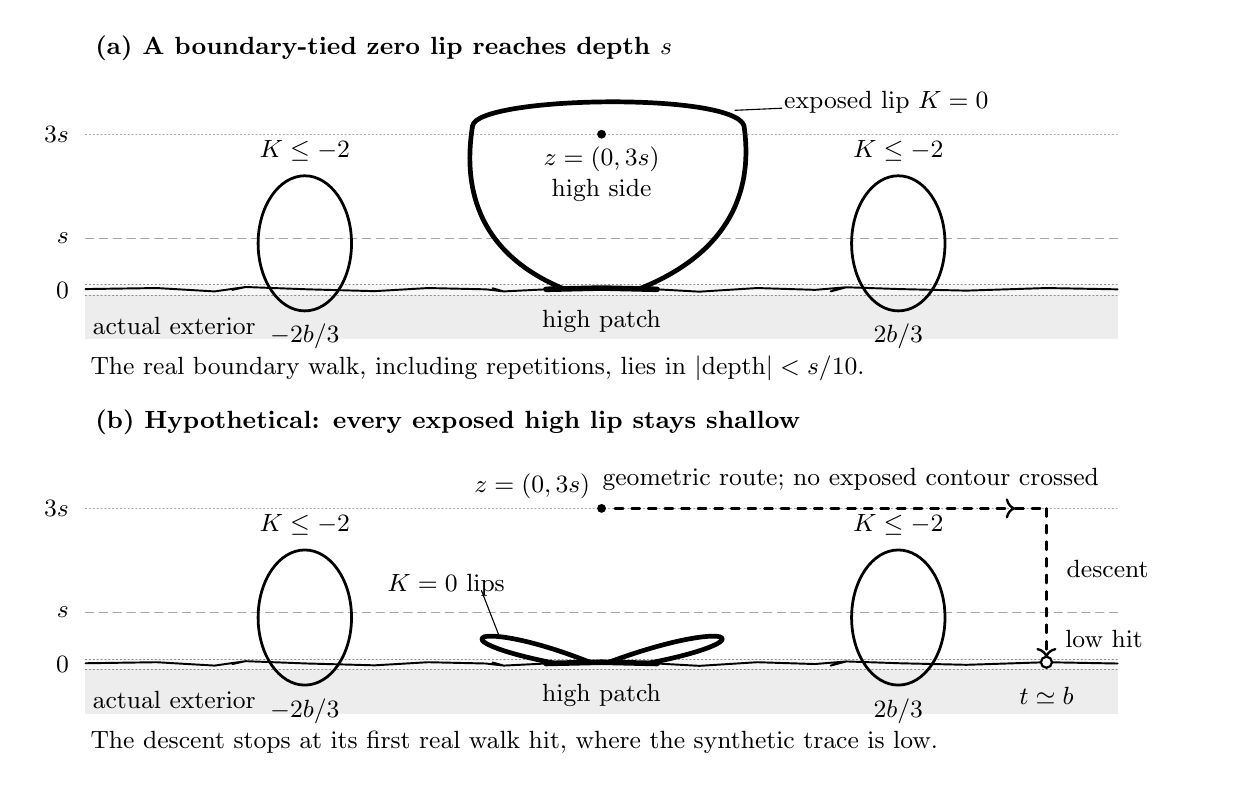
\begin{tikzpicture}[x=5.65cm,y=0.66cm,
  font=\fontsize{9}{11}\selectfont,line cap=round,line join=round]
\path[use as bounding box] (-1.29,-9.0) rectangle (1.36,5.05);
\foreach \panelshift in {0,-7.2} {
  \begin{scope}[shift={(0,\panelshift)}]
    \fill[black!7] (-1.16,-0.95) rectangle (1.16,-0.1);
    \fill[black!3] (-1.16,-0.1) rectangle (1.16,0.1);
    \draw[black!45,densely dotted] (-1.16,-0.1) -- (1.16,-0.1);
    \draw[black!45,densely dotted] (-1.16,0.1) -- (1.16,0.1);
    \draw[black!35,densely dashed] (-1.16,1) -- (1.16,1);
    \draw[black!35,densely dotted] (-1.16,3) -- (1.16,3);
    \node[anchor=east,fill=white,inner sep=1pt] at (-1.19,1) {$s$};
    \node[anchor=east,fill=white,inner sep=1pt] at (-1.19,3) {$3s$};
    \node[anchor=east,inner sep=1pt] at (-1.19,0) {$0$};
    \draw[line width=0.7pt]
      (-1.16,0.02) -- (-1.00,0.04) -- (-0.87,-0.025) -- (-0.80,0.06)
      -- (-0.83,0.005) -- (-0.80,0.06) -- (-0.66,0.015)
      -- (-0.51,-0.02) -- (-0.39,0.04) -- (-0.26,0.015)
      -- (-0.22,-0.025) -- (-0.245,0.035) -- (-0.22,-0.025)
      -- (-0.125,0.015) -- (0,0.04) -- (0.125,0.015)
      -- (0.22,-0.03) -- (0.35,0.04) -- (0.48,0.005)
      -- (0.55,0.055) -- (0.515,-0.025) -- (0.55,0.055)
      -- (0.67,0.02) -- (0.82,-0.01) -- (1,0.04) -- (1.16,0.015);
    \draw[line width=2pt] (-0.125,0.015) -- (0,0.04) -- (0.125,0.015);
    \draw[line width=1pt] (-0.667,0.9) ellipse [x radius=0.105,y radius=1.3];
    \draw[line width=1pt] (0.667,0.9) ellipse [x radius=0.105,y radius=1.3];
    \foreach \a in {-0.667,0.667} {
      \node[anchor=south,fill=white,inner sep=1pt] at (\a,2.42) {$K\le -2$};
    }
    \fill (0,3) circle [radius=1.6pt];
    \node[anchor=north] at (-0.667,-0.47) {$-2b/3$};
    \node[anchor=north] at (0.667,-0.47) {$2b/3$};
    \node[anchor=north,fill=black!7,inner sep=1pt] at (0,-0.32) {high patch};
    \node[anchor=west,inner sep=0pt] at (-1.145,-0.68) {actual exterior};
  \end{scope}
}
\node[anchor=west,font=\fontsize{9}{11}\selectfont\bfseries] at (-1.16,4.65)
  {(a) A boundary-tied zero lip reaches depth $s$};
\draw[line width=1.7pt]
  (-0.085,0.025) .. controls (-0.29,0.75) and (-0.31,2.1) .. (-0.29,3.16)
  .. controls (-0.28,3.73) and (0.29,3.82) .. (0.32,3.17)
  .. controls (0.34,2.03) and (0.30,0.76) .. (0.085,0.025);
\node[anchor=west,align=left,fill=white,inner sep=1.5pt] at (0.40,3.62)
  {exposed lip $K=0$};
\draw[thin] (0.405,3.5) -- (0.30,3.46);
\node[align=center,fill=white,inner sep=1.5pt] at (0,1.92) {high side};
\node[anchor=north,fill=white,inner sep=1.5pt] at (0,2.84) {$z=(0,3s)$};
\node[anchor=west,inner sep=0pt] at (-1.15,-1.50)
  {The real boundary walk, including repetitions, lies in $|\mathrm{depth}|<s/10$.};

\begin{scope}[shift={(0,-7.2)}]
  \node[anchor=west,font=\fontsize{9}{11}\selectfont\bfseries] at (-1.16,4.65)
    {(b) Hypothetical: every exposed high lip stays shallow};
  \node[anchor=south east,fill=white,inner sep=1.5pt] at (-0.015,3.1) {$z=(0,3s)$};
  \draw[line width=1.7pt]
    (-0.105,0.02) .. controls (-0.38,0.48) and (-0.28,0.91) .. (-0.025,0.035);
  \draw[line width=1.7pt]
    (0.015,0.035) .. controls (0.29,0.91) and (0.38,0.48) .. (0.105,0.02);
  \node[anchor=east,fill=white,inner sep=1pt] at (-0.21,1.53) {$K=0$ lips};
  \draw[thin] (-0.27,1.42) -- (-0.23,0.54);
  \draw[dashed,line width=0.85pt,->] (0.03,3) -- (0.93,3);
  \draw[dashed,line width=0.85pt,->] (1,3) -- (1,0.13);
  \draw[dashed,line width=0.85pt] (0.93,3) -- (1,3);
  \draw[fill=white,line width=0.8pt] (1,0.04) circle [radius=2pt];
  \node[anchor=south,fill=white,inner sep=2pt] at (0.56,3.23)
    {geometric route; no exposed contour crossed};
  \node[anchor=west,fill=white,inner sep=1.5pt] at (1.035,1.83) {descent};
  \node[anchor=west,inner sep=1pt] at (1.035,0.49) {low hit};
  \node[anchor=north,inner sep=1pt] at (1,-0.38) {$t\simeq b$};
  \node[anchor=west,inner sep=0pt] at (-1.15,-1.50)
    {The descent stops at its first real walk hit, where the synthetic trace is low.};
\end{scope}
\end{tikzpicture}

 \caption{The local attachment geometry, schematically and not to
 scale.  In the application to Proposition~\ref{prop:boundary-arch},
 the box lies near $(2\ell,0)$ in the untouched band
 $Q_{5\ell}\setminus Q_\ell$, away from the preliminary separators.
 Every local branch of the real boundary walk lies in the shallow
 tolerance band.  The high synthetic trace is in $[-1,0]$, the
 remaining trace in $[-3,-2]$.  Low ambient site circuits enclose the
 shallow cross-section near $t=\pm2b/3$.
 (a) An exposed zero lip attached to the high patch rises to depth
 $s$; ``high side'' is a contour-side designation, not a sign
 assertion for $K(z)$.
 (b) If every such lip stays shallow, the dashed geometric route
 reaches its first real low-trace site without crossing an exposed
 contour.  Unexposed closed contours remain integrated in the Gibbs
 law.  The exterior is joined only after a real attachment is obtained.}
 \label{fig:boundary-attachment}
\end{figure}
\FloatBarrier

\subsection{From attachments to many-scale boundary arches}

The local attachment will be joined to other attachments by paths in
the free bulk.  We establish that second ingredient before iterating
the construction across scales.

\begin{lemma}[Nonnegative paths through bulk tubes]
\label{boundary:bulk-tubes}
Consider a bounded face of a connected fixed skeleton, with its weighted
height law and usable trace at least $-2$.  Fix a finite network of
tubes in that face with positive widths and clearance from the skeleton.
Their lengths, widths and clearances are specified by fixed ratios.
For all sufficiently small meshes, the probability that every requested
tube is traversed in its prescribed direction by a site path of heights
at least zero is bounded below by a positive constant depending only
on $x$ and the network geometry.  The bound is uniform over the shape
of the skeleton outside these clearances and over its prescribed trace.
\end{lemma}

\begin{proof}
Compare from below with the flat trace $-2$ on the connected bounding
skeleton.  Realize this flat problem by
constant spin pins in the ambient graph.  In an allocated annulus
around a tube ball, ask for at least three nested good first-color
circuits with alternating signs, using disjoint buffers.  The
conditional buffer estimates give positive probability.  Constancy
of the other color on the connected skeleton is first imposed as
equality.  Its single component label is fair conditional on the
first color and its statuses.  Prescribing that label therefore leaves
the circuit-search probability unchanged.  Between successive
opposite-sign circuits there are enclosing first-color
walls, so there are at least two enclosing height loops in the
allocated annulus.  The loops lie wholly in the free bulk.

Let $E$ be the event that at least two enclosing height loops lie
wholly in the allocated annulus.  This event depends only on the
unoriented geometry and contains the alternating-color circuit event,
so its probability has the same positive lower bound.  Condition now
only on unoriented geometry in $E$.  Choose two consecutive enclosing
loops in the annulus by a deterministic rule, ordered from outer to
inner.  All loop jumps are
independent fair signs under the flat boundary, by
Lemma~\ref{lem:height-order}.  The height outside the first chosen
loop is $-2$ plus a symmetric sum of other signs, and hence is at
least $-2$ with probability at least $1/2$.  Independently, both
chosen jumps are positive with probability $1/4$.  With probability
at least $1/8$ their inner lip therefore supplies a surrounding
site circuit of height at least zero.  Each loop's two site lips
have constant heights: at every trivalent vertex on the loop the
third edge is unoccupied, joining the same-height sites along each
lip.  Loops not enclosing the
target ball cannot change this lip height.  A surrounding site
circuit can be extracted from its connected site walk.

The allocated annuli can be chosen so that successive surrounding
site circuits must intersect.  For example take equal inner radii
$a$, outer radii $2a$, and successive center distance $3a/2$.
The enclosed inner disks overlap, whereas either inner disk has a
portion beyond the other outer disk; disjoint surrounding circuits
could consequently be neither unnested nor nested.  After small
fixed changes to the radii for lattice rounding, planarity forces
an intersection.  Finite strings of these annuli give the desired
tube paths.  Each surrounding-height-circuit event is increasing,
so height association multiplies their lower bounds, first in the
flat problem and then in the actual problem by height comparison.
Only finitely many balls are needed for the fixed tube network.
\end{proof}

\begin{samepage}
\begin{proposition}[Boundary arch estimate]\label{prop:boundary-arch}
There are constants $L>100$, $c,C>0$ and a positive slope tolerance
such that the following holds.  Fix $p\in\partial D$ and a local
radius $R$ satisfying that tolerance.  Suppose the actual prescribed
trace on $S_{0,\delta}$ is at least $-1$ everywhere and at least zero
in $Q_R(p)\setminus Q_r(p)$.  Choose any $N$ positive scales
\[
 16r\le\ell_1,\qquad
 L\ell_j\le\ell_{j+1},\qquad
 \ell_N\le R/10.
\]
At all sufficiently small meshes,
\begin{equation}
 \Prob\!\left(
 \begin{array}{c}
 \text{a site circuit in }\widehat{\mathcal O}_0(H)
 \text{ surrounds }Q_r(p)\\[-2pt]
 \text{and is contained in }Q_R(p)\setminus Q_r(p)
 \end{array}\right)
 \ge 1-Ce^{-cN}.
 \label{boundary:arch-estimate}
\end{equation}
The constants are independent of $N,p$ and the prescribed trace;
the required mesh threshold may depend on the chosen positive
scales and the boundary approximation.  The same assertion holds
with all inequalities reversed when the original trace is at most
$1$ everywhere and at most zero in the clean annulus.  All usable
sites of the resulting arch have their real height at least zero,
or at most zero in the reversed assertion.
\end{proposition}
\end{samepage}

\begin{proof}
We give the increasing construction.  All choices of relative widths
below are fixed once and for all, depending at most on $x$.

\paragraph{Preliminary blocks at level $-1$.}
In block $j$ seek site circuits of level at least $-1$ in the two
strips
\[
 Q_{\ell_j}\setminus Q_{\ell_j/2},
 \qquad Q_{7\ell_j}\setminus Q_{5\ell_j},
\]
with artificial exterior allowed, each surrounding its inner box.
Use Lemma~\ref{boundary:synthetic-trace} with high intervals on the
two clean boundary subarcs running through \emph{all} these strips.
Place their transitions before the innermost buffers and beyond
the outermost ones, in the available clean annulus.  Low intervals
are used on the remaining skeleton.  There are only two high arcs,
so the number $M$ of transition labels is independent of $N$.

Before imposing those labels, the slightly narrower buffers in
each strip see only favorable first-color pins.  By
Lemma~\ref{lem:buffer-circuits} there is $a_1>0$ such that, given
the earlier complete first-color/status slot records, both good
plus circuits in the next block occur with conditional probability
at least $a_1$.  All such buffers are disjoint by the choice of $L$.
A good circuit meets a high boundary arc, since that arc traverses
the strip.  Its adjacent site path is consequently in the anchored
pair $\{-1,0\}$.  That path has winding number one around the inner
box; erasing unnecessary pieces gives a simple surrounding site
circuit at level at least $-1$.

If $I_j$ records the two-circuit success, the conditional estimate
implies, for $t>0$,
\[
 \E\exp\!\left(-t\sum_{j=1}^N I_j\right)
 \le(1-a_1+a_1e^{-t})^N.
\]
Choosing $t$ and then a sufficiently small $a_2>0$ gives
$\Prob(\sum I_j<a_2N)\le e^{-c_1N}$.
Conditioning on the bounded number of transition labels multiplies
this failure bound by at most $2^M$.  Thus with probability at least
$1-C_1e^{-c_1N}$ at least $a_2N$ blocks have both site circuits.
The event that at least this many blocks succeed is increasing in
the heights.  Height comparison transfers the entire count estimate
to the actual law, without conditioning successively on synthetic
events in that law.

In each actual successful block select an innermost circuit in the
inner strip and an outermost circuit in the outer strip.  Reveal
the unsuccessful strips and every nonretained region.  By
Lemma~\ref{boundary:extremal}, conditional on this record
$\mathcal R$, all retained middle components have independent height
Gibbs laws.  Their skeleton is the base skeleton together with the
real portions of the two selected circuits.  Each circuit surrounds
a boundary-centered box containing a point a fixed positive distance
outside $D$.  A site circuit lying wholly in the real domain would
have its geometric interior in the simply connected $D_\delta$,
so each selected circuit visits the genuine exterior.  Every maximal
real run along it therefore ends at a transition to the exterior;
its endpoint is a site of the original boundary face layer.  Thus
every connected real portion meets the base skeleton.  There can be
arbitrarily many such real portions.  In either local attachment
comparison they all meet low base sites, since the high patch lies
in the untouched middle band.  They can therefore be adjoined to
the existing low parts without creating new parts or new transition
labels, exactly as in Lemma~\ref{boundary:synthetic-trace}.
The resulting prescribed graph is connected.  Its usable values are
at least $-1$, and in particular at least $-2$; allowing an extra observed
outer rounding layer would give the same latter bound.  We do not
expose any additional layer on the retained side.  The band
$Q_{5\ell_j}\setminus Q_{\ell_j}$ is untouched, and its original
base boundary has height at least zero.

\paragraph{Upgrading a retained block.}
For clarity suppress the index $j$.  Put attachment boxes near the
two boundary positions with tangential coordinate $\pm2\ell$.
Choose $b$ to be a small fixed fraction of $\ell$, then
$s=\lambda b$ as in Lemma~\ref{lem:boundary-attachment}.  Use the
local reference height of the limiting boundary in each box.
Both boxes lie in $Q_{5\ell}\setminus Q_\ell$, away from the
preliminary separators.  Choose the slope tolerance so small that
the limiting arc varies by less than $s/20$ within each box.  At
small enough mesh the full base skeleton, including all its
repeated branches, is in the required $s/10$ band.  These are fixed
geometric requirements before the mesh limit.  The attachment
lemma gives, uniformly conditional on $\mathcal R$, a probability
at least $a_0$ at each box.

Place a horizontal crossbar tube at depth close to $s/2$ in each
box, with depth width less than $s/10$ and ends beyond its two
sides.  It must meet every successful rise from the base band to
depth $s$: two primal lattice paths crossing a rectangle in the
two different directions share a site.  Join these crossbars by
narrow bulk tubes running upwards near tangential positions
$\pm2\ell$ and across at depth close to $2\ell$.  All widths are
positive fixed fractions of $s$, and all tubes lie in the free
part of $Q_{5\ell}\setminus Q_\ell$.
Lemma~\ref{boundary:bulk-tubes} gives a positive lower bound for their
simultaneous crossings.
The two attachments and the bulk crossings are increasing events
in the same actual conditional height law.  Height association
therefore gives their intersection probability at least a fixed
$a_3>0$.

Join the boundary ends through the clean real boundary sites to
the genuine exterior, as in the attachment lemma.  In that exterior
connect them by a path below the arc, around the lower side of
$Q_\ell$, staying in $Q_{5\ell}\setminus Q_\ell$.  The upper bulk
route and lower exterior route lie in disjoint opposite corridors,
so their union contains a closed site walk with winding number one
around $Q_\ell$.  It contains a simple surrounding open circuit.
Only sites outside the original $V_\delta$ have been used
artificially; no real preliminary separator was given artificial
height.  This produces the desired level-zero arch in the block.

Conditional on $\mathcal R$, distinct retained middle problems are
independent.  If at least $a_2N$ preliminary blocks succeeded, the
probability that none upgrades is at most $(1-a_3)^{a_2N}$.
Adding the preliminary count failure proves
\eqref{boundary:arch-estimate}.  Reflection $H\mapsto-H$ proves the
reversed assertion.  When a resulting arch is later used as a
conditioning boundary, it is searched for afresh by the height
extremal selection of Lemma~\ref{boundary:extremal}; none of the
synthetic constructions or auxiliary successes is then conditioned
on.
\end{proof}

\subsection{Vanishing brackets and boundary correlations}

The next estimate removes the mean contribution of the exceptional
windows.  After establishing compactness in Section~\ref{sec:limit},
we will combine it with the ordered bracket coupling to identify the
limiting brackets with the true field.

\begin{proposition}[Vanishing bracket means]
\label{prop:bracket-collapse}
Fix a finite regular grid as in Definition~\ref{def:brackets}.
For every $f\in C_c^\infty(D)$, the upper and lower bracket fields
satisfy
\begin{equation}
 \lim_{\epsilon\downarrow0}\ \limsup_{\delta\downarrow0}
 \left|\E H_\delta^{\pm,\epsilon}(f)\right|=0.
 \label{boundary:bracket-means}
\end{equation}
\end{proposition}

\begin{proof}
The bracket trace belongs to $[-1,1]$ and equals zero away from the
finitely many exceptional windows.  Choose pairwise disjoint fixed
outer neighborhoods of their centers, missing $\supp f$.  Given
$N$, choose $N$ separated positive scales in each neighborhood and
then take $\epsilon$ sufficiently small that its exceptional
window lies inside the innermost box.  Finally take the mesh small
with this geometry fixed.

Condition on the bracket trace.  Proposition~\ref{prop:boundary-arch}
gives increasing level-zero arches around all windows except with
probability at most $JC e^{-cN}$, where $J$ is their fixed number.
Select innermost arches by testing from the exceptional side.  On
simultaneous success every retained component meeting $\supp f$
has nonnegative usable trace: each new real separator site has
height at least zero and the old visible base trace is zero.  By
height comparison the conditional mean on each such component is
nonnegative, and hence so is their sum against a nonnegative $f$.
Thus, using the unconditional bracket moment bound
of Proposition~\ref{prop:smearing},
\[
 \E H_\delta^{\pm,\epsilon}(f)
 \ge -\|H_\delta^{\pm,\epsilon}(f)\|_2
       (JC e^{-cN})^{1/2}
 \ge -C_f e^{-cN/2}.
\]
The same argument with decreasing arches gives the upper bound.
In particular no bound conditioned on arch failure is needed.
The moment constant is uniform over the original traces in
$[-1,1]$.  Since $N$ is arbitrary, this proves
\eqref{boundary:bracket-means} for nonnegative tests.  Splitting a
smooth signed test into a difference of nonnegative smooth compactly
supported tests proves the general case.

\end{proof}

\begin{proposition}[Boundary moments with exterior spectators]
\label{prop:boundary-moments}
Fix a nonnegative smooth radial bump $\rho$, supported in the unit
disk, with integral one, and fix a sufficiently small $\theta>0$.
For $z\in D$ write $d(z)=\dist(z,\partial D)$ and
\[
 \rho_z(u)=(\theta d(z))^{-2}
       \rho\!\left(\frac{u-z}{\theta d(z)}\right),\qquad
 Y_z=H(\rho_z),
\]
where $H$ is any subsequential distributional and moment limit of
the true fields.  For every $1\le p<\infty$,
\begin{equation}
 \sup_{z\in D}\|Y_z\|_p\le C_{p,\theta,D,\rho}.
 \label{boundary:uniform-depth-moments}
\end{equation}
In particular this bound is uniform when $z$ approaches any point
of a fixed compact boundary arc.

Let $p_0\in\partial D$ and let $F$ be a product of a fixed number
of smooth averages supported a positive distance from $p_0$.
The averages may be fixed in the interior, or may be of the same
comparable-depth form with centers approaching fixed boundary
points distinct from $p_0$.  Then, jointly in those allowed
approaches,
\begin{equation}
 \E[Y_zF]\longrightarrow0\qquad(z\longrightarrow p_0).
 \label{boundary:spectator-vanishing}
\end{equation}
The same statement holds for finite linear combinations of these
products.

If $p_1,\ldots,p_m$ are distinct fixed boundary points and
$z_i\to p_i$, then the reference average
$Z_m=m^{-1}\sum_{i=1}^mY_{z_i}$ satisfies
\begin{equation}
 \limsup_{z_i\to p_i}\|Z_m\|_2\le C m^{-1/2},
 \qquad \sup_m\sup_{z_1,\ldots,z_m}\|Z_m\|_p\le C_p.
 \label{boundary:reference-average}
\end{equation}
In the first assertion $m$ and its distinct boundary points are
fixed before taking the depth limits.  Subsequently $m\to\infty$
makes these references tend to zero in every finite $L^p$.
\end{proposition}

\begin{proof}
At mesh $\delta$ put $Y_{z,\delta}=h_\delta(\rho_z)$, and denote the
corresponding lattice spectator product by $F_\delta$.
At a fixed $z$, the distance from its lattice representative to the
prescribed skeleton tends to $d(z)$.  The exact face-area weights
of $\rho_z$ have total mass one, are supported in a ball of radius
$\theta d(z)+O(\delta)$, and are bounded by a constant times
$(\delta/d(z))^2$.  The ratio between boundary distance and smearing
radius is thus bounded above and below independently of $z$ once
the mesh is taken sufficiently small for that fixed placement.
Proposition~\ref{prop:smearing}, with original trace zero, gives
\eqref{boundary:uniform-depth-moments}.  The passage to the limit
uses the higher moments from the same proposition.  Compactness
of the smooth boundary makes its constants uniform over boundary
points; no estimate uniform in the approximation error divided by
a moving depth is asserted before taking the mesh limit.

Choose a small fixed outer neighborhood of $p_0$ missing all the
spectator supports; for approaching spectators this is possible
uniformly once their limiting distinct points have been fixed.
Given $N$, choose $N$ fixed separated scales inside this neighborhood.
For all sufficiently close $z$ the support of $\rho_z$ is in the
inner box of this stack.  Apply
Proposition~\ref{prop:boundary-arch} to the true zero boundary.
Select an outermost increasing arch by testing from outside and
reveal its exterior and real trace.  The spectator product $F_\delta$,
including its absolute height values, is measurable in that exterior
record.  On success, the retained region containing the testing
ball has nonnegative usable trace, and hence nonnegative conditional
mean for its unit nonnegative average.  For any nonnegative
exterior-measurable factor $U$ it follows that
\[
 \E[Y_{z,\delta}U]
 \ge -\E\big[|Y_{z,\delta}|U\ind_{\{\text{increasing search fails}\}}\big].
\]
The separate decreasing search gives the corresponding upper bound.
These searches reveal only their tested sides; they do not
condition on the intermediate constructions in the arch proof.

Apply the two bounds to $U=(F_\delta)_+$ and $U=(F_\delta)_-$, the positive and
negative parts of the whole spectator product.  If $F$ has $k$
factors, H\"older's inequality and the unconditional
$2(k+1)$-moment bounds give
\[
 \E\big[|Y_{z,\delta}F_\delta|\ind_{\{\text{a search fails}\}}\big]
 \le \|Y_{z,\delta}F_\delta\|_2\,
       \Prob(\text{a search fails})^{1/2}
 \le C_F e^{-cN/2}.
\]
The constants remain bounded for comparable-depth spectators at
the other fixed boundary points, by
\eqref{boundary:uniform-depth-moments}.  In particular the estimate
uses moments in the original zero-boundary law, not moments under
a failure event or a random high trace.  First take the mesh limit
at fixed positions and scales.  Then take the indicated approaches
to the distinct boundary points.  The resulting limsup is at most
$C_F e^{-cN/2}$.  Since $N$ was arbitrary, this proves
\eqref{boundary:spectator-vanishing}.

Finally, \eqref{boundary:uniform-depth-moments} bounds the diagonal
terms in $\E Z_m^2$ by $C/m$.  Each of the finitely many off-diagonal
terms vanishes as the depths tend to zero, by
\eqref{boundary:spectator-vanishing} with one spectator.  This proves
the first assertion of \eqref{boundary:reference-average}.
Minkowski's inequality gives its uniform $L^p$ bounds independently
of $m$.  Interpolation between $L^2$ and any larger finite moment
then proves the final claim; for $p\le2$ use monotonicity of
$L^p$ norms.  These are absolute-height references, with no lift
constant left unspecified.
\end{proof}

\section{Identification of the limiting field}
\label{sec:limit}

Fix \(x\) throughout, and let \(v\in(0,\infty)\) be the
domain-independent constant in Proposition~\ref{prop:plane-covariance}.
We identify every subsequential limit of the actual zero-boundary
fields.  The steps below also establish tightness and justify passage
of all moments; no assertion of Gaussianity is used before the last
step.

\subsection{Compactness, moments, and the insertion identity}

We write \(h_\delta(f)=\int_D h_\delta(z)f(z)\dd z\).
This is the exact face-area pairing from the introduction, including
for signed tests.  In particular \(\int f=0\) means that its discrete
weights sum to exactly zero, so adding a constant to a height lift has
no effect.

\begin{proposition}[Tightness and moment convergence]
\label{prop:tightness}
For every \(t>1\), the true fields are tight in
\(H^{-t}_{\mathrm{loc}}(D)\).  The same holds for the upper and lower
brackets, uniformly in their exceptional windows.  Every fixed finite
collection of test pairings has uniformly bounded moments of every
order.  Along a distributional law limit, all its mixed moments
converge.  These assertions hold also for finite joint couplings of
the indicated fields.
\end{proposition}

\begin{proof}
A consequence of Proposition~\ref{prop:smearing}, using a finite
cover of a compact set by interior disks, is
\begin{equation}
 \sup_\delta\|h_\delta(f)\|_{L^p}
 \le C_{K,p}\|f\|_\infty,\qquad
 \supp f\subset K\Subset D,\quad 1\le p<\infty.
 \label{eq:limit-fixed-moments}
\end{equation}
Indeed, split the face weights by a smooth partition of unity
subordinate to that cover.  Each resulting weight family has bounded
total variation and the required maximum weight on its fixed disk;
apply the smearing estimate and the triangle inequality.  The argument
applies to the brackets after conditioning on their traces, whose
values lie between \(-1\) and \(1\).  Its constants thus do not depend
on the windows.  Complex tests are handled by their real and imaginary
parts.

Here is the compactness argument in detail.  Place \(D\) in a square
torus and fix \(\chi\in C_c^\infty(D)\).  For its Fourier basis
\(e_k\), \(k\in\Z^2\), let
\(a_{\delta,k}=h_\delta(\chi\overline{e_k})\).  Since the moduli of the
basis functions are constant, \eqref{eq:limit-fixed-moments} bounds
\(\|a_{\delta,k}\|_{L^p}\) independently of \(k\).  For \(s>1\) and
\(p\ge2\), Minkowski's inequality gives
\begin{align}
 \bigl\|\|\chi h_\delta\|_{H^{-s}}^2\bigr\|_{L^{p/2}}
 &\le
 \sum_{k\in\Z^2}(1+|k|^2)^{-s}
             \|a_{\delta,k}\|_{L^p}^2
 \le C_{\chi,p,s}.
 \label{eq:limit-sobolev-moments}
\end{align}
The bounds for smaller \(p\) follow by monotonicity of \(L^p\) norms.
Choose \(1<s<t\).  A bounded \(H^{-s}\) ball is relatively compact
in \(H^{-t}\): its Fourier tail beyond frequency \(M\) has squared
\(H^{-t}\) norm at most
\((1+M^2)^{-(t-s)}\) times its squared \(H^{-s}\) norm, and its
first finitely many coordinates lie in a bounded finite-dimensional
set.  Markov's inequality and \eqref{eq:limit-sobolev-moments}
therefore give tightness of \(\chi h_\delta\) in \(H^{-t}\).

Choose nested interior compacts exhausting \(D\), and smooth cutoffs
equal to one on successive compacts.  For any prescribed error
probability, choose a compact set for the \(n\)-th cutoff with error
at most that probability times \(2^{-n}\).  The simultaneous
localizations then lie in a relatively compact set for the local
\(H^{-t}\) topology.  This proves the stated local tightness.
Equivalently, this topology is the compatible subspace of a countable
product of the localized Sobolev spaces, with its usual metrizable
topology.  The same argument and a union bound treat finite joint
couplings.

For fixed \(f_1,\ldots,f_k\), a monomial
\(\prod_i h_\delta(f_i)^{a_i}\) has uniformly bounded \(L^{1+\epsilon}\)
norm, for instance with \(\epsilon=1\), by
\eqref{eq:limit-fixed-moments} and H\"older's inequality at sufficiently
high orders.  Its uniform integrability, joint convergence of the
pairings, and truncation prove convergence of that mixed moment.
The same argument gives moment convergence with bounded continuous
functions of finitely many pairings.  In particular all the preceding
moment bounds pass to every limit.
\end{proof}

A second consequence of the smearing estimate, which we will use at
collisions, is the following.  If
\(f_{z,r}(w)=r^{-2}f((w-z)/r)\), where \(f\) ranges over a fixed bounded
family of smooth functions supported in a fixed disk, then on an
interior compact, for sufficiently small \(r\),
\begin{equation}
 \|h_\delta(f_{z,r})\|_{L^p}
 \le C_{p,f}\bigl(1+\log(1/r)\bigr)^{1/2}.
 \label{eq:limit-small-moments}
\end{equation}
It suffices here and below to take the mesh sufficiently small at each
fixed \(r\).  Proposition~\ref{prop:smearing} gives this bound since
the distance to the boundary is bounded below and the smearing radius
is \(r\).  It passes to limits by Proposition~\ref{prop:tightness}.
For plane fields and zero-total \(f\), Proposition~\ref{prop:plane-moments}
instead gives a bound independent of \(r\).

Fix henceforth any subsequence on which the true fields converge,
and denote its limit by \(H\).  Height reflection and moment
convergence imply \(\E H(f)=0\).

\begin{lemma}[Transfer to the chosen field]
\label{limit:transfer}
The field \(H\) satisfies the limiting insertion identity of
Proposition~\ref{prop:bracket-insertion} in every disk arrangement
allowed there:
\begin{equation}
 \E\left[H(\Delta\varphi)
          \prod_{\ell=1}^k H(g_\ell)\right]=0,
 \qquad \int g_\ell=0,
 \label{eq:limit-insertion}
\end{equation}
where each \(g_\ell\) is supported in its indicated spectator disk.
The same assertion first holds with each spectator replaced by a
bounded continuous function of finitely many zero-total tests in that
disk.
\end{lemma}

\begin{proof}
Fix a finite grid of regular horizontal levels and positive exceptional
windows sufficiently small for the given arrangement.  We pass first
to the mesh limit and then to the window limit, keeping the chosen
true-field marginal throughout.

Couple its lower and upper brackets with the true field in order,
as in Lemma~\ref{pins:bracket-order}.  First take a joint law limit
along the chosen subsequence, with the windows fixed.  Next shrink
the windows and take a further joint limit.  Proposition~\ref{prop:tightness}
applies uniformly throughout, so these extractions are possible and
the middle marginal is always the already chosen law of \(H\).
Distributional order passes to the limits because evaluation against
each nonnegative smooth test is continuous.  Write the resulting
ordered triple as
\[
       H^-\le H\le H^+.
\]
Proposition~\ref{prop:bracket-collapse} and moment convergence give
\(\E H^-(f)=\E H^+(f)=0\), as well as \(\E H(f)=0\).
For every nonnegative smooth \(f\), both nonnegative random variables
\(H^+(f)-H(f)\) and \(H(f)-H^-(f)\) thus have expectation zero.
Apply this to a countable dense family of nonnegative tests on an
exhaustion of \(D\).  Continuity of distributions then shows
\(H^-=H=H^+\) almost surely as distributions.

At fixed windows, Proposition~\ref{prop:bracket-insertion} gives the
insertion identity for bounded local increment factors.  For bounded
continuous functions of zero-total pairings it passes to the first
law limit by uniform integrability of \(H(\Delta\varphi)\), and then
to the window limit by the same argument.  The collapsed marginal is
the chosen \(H\), so this proves that identity for \(H\).
Repeat for any desired finite grid; no change to the chosen marginal
is involved.  Finally truncate each \(H(g_\ell)\) by a bounded
continuous truncation.  H\"older's inequality and moments of orders
larger than the number of factors show that the expectation of the
truncation error tends to zero.  This proves
\eqref{eq:limit-insertion}.
\end{proof}

\subsection{Boundary references and harmonic moment distributions}

The insertion identity currently permits only zero-total spectator
tests.  To obtain harmonicity of the full moment distributions, we
must allow arbitrary tests, including averages of absolute heights.
We construct reference averages that vanish near the boundary;
subtracting such a reference expresses each spectator as a finite
sum of local zero-total observations.

Fix a nonnegative smooth radial bump \(\rho\) of integral one,
supported in the unit disk.  All unit radial averages below are
translations and dilations of this bump.

\begin{lemma}[Vanishing references]
\label{limit:references}
There are finite averages \(R_m\) of unit radial pairings of \(H\),
supported arbitrarily near the boundary, such that
\[
       \|R_m\|_{L^p}\longrightarrow0
       \quad\text{for every }p<\infty.
\]
Each \(R_m\) uses finitely many distinct boundary points, with depth
chosen after those points are fixed.  Its constituent disks can be
required to have any prescribed small positive maximum diameter.
\end{lemma}

\begin{proof}
Choose distinct points \(p_1,\ldots,p_m\) on a fixed boundary arc.
For small \(a>0\), put the centers a distance \(a\) along their inward
normals and use bumps \(\psi_{\ell,a}\) of radius \(\theta a\), where
\(0<\theta<1/4\) is fixed.  The tubular neighborhood theorem for a
\(C^2\) Jordan curve gives distance exactly \(a\) to the boundary for
these centers when \(a\) is sufficiently small.  Define
\[
 Y_{\ell,a}=H(\psi_{\ell,a}),\qquad
 R_{m,a}=\frac1m\sum_{\ell=1}^m Y_{\ell,a}.
\]
The comparable-depth moment bound in
Proposition~\ref{prop:boundary-moments} is uniform along this fixed
arc.  Minkowski's inequality therefore gives
\(\sup_{m,a}\|R_{m,a}\|_{L^q}\le C_q\) for each finite \(q\), after
restricting to the corresponding sufficiently small depths.
For fixed \(m\), the same proposition gives
\(\E[Y_{\ell,a}Y_{k,a}]\to0\) when \(\ell\ne k\).
Consequently
\begin{equation}
  \limsup_{a\downarrow0}\|R_{m,a}\|_{L^2}^2
       \le \frac{C_2^2}{m}.
  \label{eq:limit-reference-second}
\end{equation}
For each \(m\), choose a positive depth \(a_m\) small enough that this
squared norm is at most \((C_2^2+1)/m\) and all disk diameters meet
the prescribed bound.  Then \(R_m=R_{m,a_m}\) tends to zero in
\(L^2\).  For \(p>2\), interpolate this convergence with the uniform
\(L^q\) bound for any \(q>p\); for \(p\le2\), use monotonicity.
This proves the assertion.  The order in
\eqref{eq:limit-reference-second} is depth first at fixed \(m\),
then \(m\to\infty\).
\end{proof}

For \(j\ge1\), define the moment distribution \(T_j=\E H^{\otimes j}\)
on \(D^j\), and set \(T_0=1\).  This definition is legitimate for
general smooth tests on the product, not just tensor tests.
For example, after localizing in a square torus, expand a product-space
test in its Fourier series.  Its coefficients decay faster than any
power, while H\"older's inequality and
\eqref{eq:limit-fixed-moments} bound the expected absolute product of
any \(j\) Fourier coefficients uniformly.  The resulting series is
absolutely convergent and defines a continuous distribution.
For tensor tests it gives precisely
\[
 T_j(f_1\otimes\cdots\otimes f_j)
       =\E\prod_{i=1}^j H(f_i).
\]
This construction agrees with taking the expectation of the tensor
power of the random distribution by
\eqref{eq:limit-sobolev-moments}.

For \(j\ge2\), we will determine \(T_j\) from \(T_{j-2}\) by its behavior
in one variable.  The next steps establish harmonicity away from coincident
points, rule out additional distributions supported at coincidences,
and identify each logarithmic collision coefficient.  Together with
the zero boundary value, these properties will give the Gaussian
moment recursion by subtraction of Dirichlet Green functions.

\begin{proposition}[Harmonic moments]
\label{prop:harmonic-moments}
Let
\[
 \mathcal C_j=\{(z_1,\ldots,z_j)\in D^j:
                         z_i\ne z_k\text{ for }i\ne k\}.
\]
On \(\mathcal C_j\), \(T_j\) is a smooth function and is harmonic in
each variable separately.
\end{proposition}

\begin{proof}
We prove the first-variable distributional Laplace identity in a
small product neighborhood of any distinct tuple; symmetry then gives
all the identities.  Translate the first center to the origin.
Choose \(R>0\) so that \(B(0,4R)\Subset D\) and all the other centers
lie outside \(\overline{B(0,4R)}\).  Choose \(0<b<R/1000\) and
\(0<\eta<R/(1000j)\).  Fix the finite regular grid supplied by
Lemma~\ref{pins:local-geometry} for \(z_0=0\), \(\rho=R\), and
\(q=j-1\).  Its choice is independent of the small spectator disks
and chains constructed below.
Take \(\varphi\) supported in \(B(0,b)\), and take each spectator
test \(f_i\), \(2\le i\le j\), in a sufficiently small neighborhood
of its center, of diameter less than \(\eta/4\).
We will show
\begin{equation}
       \E\left[H(\Delta\varphi)\prod_{i=2}^j H(f_i)\right]=0.
       \label{eq:limit-harmonic-tensor}
\end{equation}
For \(j=1\) this follows from the zero mean; suppose \(j\ge2\).

Write \(c_i=\int f_i\), and choose a unit bump \(\rho_i\) in that
spectator neighborhood.  Take a reference \(R_{m,a}\) from the
preceding lemma, at a fixed positive depth small enough that all
its disks have diameter less than \(\eta/4\) and lie outside
\(\overline{B(0,4R)}\).  This is possible because that closed ball
is a compact subset of \(D\), whereas the reference disks can be
placed arbitrarily near the boundary.
Every center can be joined to each reference center by a finite path
in \(D\setminus\overline{B(0,R)}\).  To verify this last geometric
point, start with a polygonal path in the connected open set \(D\).
Whenever it enters the protected disk, replace that portion by an
arc in \(B(0,2R)\setminus\overline{B(0,R)}\); this annulus lies in
\(D\).  A small perturbation and a finite subdivision give a path
with compact image and positive clearance from both the protected
disk and the boundary.

Along each such path choose a finite chain of smooth unit bumps,
beginning with \(\rho_i\) and ending with \(\psi_{\ell,a}\).
Make the step lengths and bump radii so small that the union of
two consecutive supports is contained in a disk of radius less
than \(\eta\), disjoint from \(\overline{B(0,R)}\).
If necessary interpolate their radii in finitely many steps near
the endpoints.  Telescoping yields
\[
 H(f_i)-c_iH(\psi_{\ell,a})
  =H(f_i-c_i\rho_i)
    +c_i\sum_{\text{chain}}H(\rho_{\mathrm{old}}-\rho_{\mathrm{new}}).
\]
Every summand on the right is a zero-total test in one of these
small disks.  Averaging this equality over \(\ell\) expresses
\(H(f_i)-c_iR_{m,a}\) as a finite linear combination of such
observations.

Expand the product of these \(j-1\) finite sums.  Each monomial
selects at most \(j-1\) spectator disks, whatever the number or
length of the chains.  The insertion support lies in
\(B(0,R/1000)\), and every selected disk is outside \(B(0,R)\)
with radius less than \(R/(1000j)\).  These are precisely the
hypotheses for the grid already fixed from
Lemma~\ref{pins:local-geometry}.  For each monomial its two selected
levels give the oblique separation of the middle-strip boundary
pieces and spectators needed by Proposition~\ref{prop:bracket-insertion}.
The pair of levels may depend on the monomial; the grid does not.

There are only finitely many monomials.  Choose the exceptional windows
small enough to preserve all their positive margins.
Lemma~\ref{limit:transfer} gives zero expectation for each monomial
with the insertion.  Summing these exact identities gives
\begin{equation}
 \E\left[H(\Delta\varphi)
              \prod_{i=2}^j\bigl(H(f_i)-c_iR_{m,a}\bigr)\right]=0.
 \label{eq:limit-subtracted-references}
\end{equation}
All disks, chains, tests and grid levels used to obtain this equality
are finite and fixed before using the limiting insertion identity.

It remains to remove the reference.  This error is estimated before
the chain expansion.  The algebraic difference between the product
in \eqref{eq:limit-subtracted-references} and \(\prod_iH(f_i)\)
is a sum of \(j-1\) terms, each containing one factor \(c_iR_{m,a}\)
and other factors of the form \(H(f_k)\) or
\(H(f_k)-c_kR_{m,a}\).  H\"older's inequality and the uniform
moment bounds give, for some finite \(p\) depending only on \(j\),
\[
 \left|\E H(\Delta\varphi)
       \left\{\prod_{i=2}^jH(f_i)
        -\prod_{i=2}^j(H(f_i)-c_iR_{m,a})\right\}\right|
       \le C\|R_{m,a}\|_{L^p}.
\]
The constant does not count chain terms.  Choose depths and then
\(m\) as in Lemma~\ref{limit:references}; the right side tends to
zero.  This proves \eqref{eq:limit-harmonic-tensor}.

Finite sums of tensor tests are dense in the test-function space
on each such product neighborhood, for example by a localized
Fourier expansion with convergence of every derivative.
Consequently \(\Delta_{z_1}T_j=0\) there as a distribution.
Symmetry gives all \(j\) separate Laplace equations.  Their sum is
the ordinary elliptic Laplacian on \(\R^{2j}\); the local regularity
theorem for harmonic distributions makes \(T_j\) smooth there.
The separate distributional equations then hold pointwise.
\end{proof}

\begin{lemma}[No distributions supported on collisions]
\label{lem:no-diagonal}
On every compact subset of \(D^j\), the off-diagonal function from
Proposition~\ref{prop:harmonic-moments} is locally integrable and
represents all of \(T_j\).  For \(j\ge2\), if
\(d(\mathbf z)=\min_{i<k}|z_i-z_k|\), then, locally away from
the boundary,
\begin{equation}
 |T_j(\mathbf z)|
 \le C\bigl(1+\log_+(1/d(\mathbf z))\bigr)^{j/2},
 \qquad \mathbf z\in\mathcal C_j.
 \label{eq:limit-log-bound}
\end{equation}
Moreover, for distinct fixed \(z_2,\ldots,z_j\in D\),
\begin{equation}
 T_j(z_1,z_2,\ldots,z_j)\longrightarrow0
        \quad\text{as }z_1\longrightarrow p\in\partial D.
 \label{eq:limit-zero-boundary}
\end{equation}
\end{lemma}

\begin{proof}
Let \(T_{j,h}\) be the convolution of \(T_j\) with a product of
\(j\) radial unit bumps of common radius \(h\), considered on a
fixed interior compact and with \(h\) small enough to remain in
\(D\).  By H\"older's inequality and
\eqref{eq:limit-small-moments},
\begin{equation}
 |T_{j,h}(\mathbf z)|
   =\left|\E\prod_{i=1}^jH(\rho_{z_i,h})\right|
   \le C(1+\log(1/h))^{j/2},
 \label{eq:limit-mollifier-bound}
\end{equation}
including at coincident centers.  Whenever \(d(\mathbf z)>2h\),
the product of bump supports is off the diagonals.  The radial mean
value property, successively in each harmonic variable, gives
\(T_{j,h}(\mathbf z)=T_j(\mathbf z)\).
Taking \(h\) to be the smaller of \(d(\mathbf z)/4\) and a fixed
interior radius proves \eqref{eq:limit-log-bound}.

For completeness, a collision tube
\[
       A_h=\{\mathbf z:d(\mathbf z)\le2h\}
\]
in a fixed compact set has volume at most \(C_jh^2\): use the
union bound over pairs, fix all but one point in a selected pair,
and integrate that point over a disk of radius \(2h\).
The same bound at every radius \(s\), followed by integration of
the distribution function, gives for \(q\ge0\)
\[
 \int_{A_h}\bigl(1+\log_+(1/d(\mathbf z))\bigr)^q\dd\mathbf z
       \le C_qh^2(1+\log(1/h))^q.
\]
Indeed for \(q>0\), integrate
\(q(1+\log(1/s))^{q-1}\dd s/s\) against the bound \(Cs^2\);
the endpoint term is \(Ch^2(1+\log(1/h))^q\).
This proves local integrability.  It also shows that the
off-diagonal function has vanishing \(L^1\) mass on \(A_h\).
Equation~\eqref{eq:limit-mollifier-bound} gives the same assertion
for \(T_{j,h}\), since \(h^2(1+\log(1/h))^{j/2}\to0\).
Off \(A_h\) the two functions agree exactly.  Thus \(T_{j,h}\)
converges locally in \(L^1\) to the off-diagonal function.
But convolution also converges to \(T_j\) in distributions.
These limits are equal.  In particular neither a delta distribution
nor any of its derivatives on a collision diagonal can be present.
The case \(j=1\) has no collision set and follows directly from
harmonicity.

To prove \eqref{eq:limit-zero-boundary}, choose disjoint small fixed
radial averaging disks around \(z_2,\ldots,z_j\).
For \(z_1\) near \(p\), choose its averaging radius to be
\(\theta\dist(z_1,\partial D)\).
The supports are pairwise separated.  The harmonic mean value
property in every variable identifies the displayed pointwise
value with
\[
 \E\left[H(\rho_{z_1,\theta\dist(z_1,\partial D)})
                         \prod_{i=2}^jH(\rho_{z_i,s_i})\right].
\]
Proposition~\ref{prop:boundary-moments} makes this tend to zero.
For \(j=1\) the same conclusion also follows from the zero mean.
\end{proof}

\subsection{The logarithmic collision coefficient}

\begin{lemma}[Punctured harmonic expansion]
\label{limit:puncture}
Let \(j\ge2\).  Fix a collision point \(y\in D\) and distinct spectators
\(\mathbf z=(z_3,\ldots,z_j)\), all separated from \(y\).
For \(x\) in a sufficiently small punctured disk about \(y\),
\begin{equation}
 T_j(x,y,\mathbf z)
      =L(y,\mathbf z)\log(1/|x-y|)
                           +R(x;y,\mathbf z),
 \label{eq:limit-puncture}
\end{equation}
where \(R\) extends harmonically across \(x=y\).
The coefficient \(L\) is smooth in the separated parameters
\((y,\mathbf z)\), and the first-variable derivatives of \(R\)
are bounded uniformly on smaller disks and compact sets of these
parameters.  The coefficient \(L\) is separately harmonic in each
spectator variable.
\end{lemma}

\begin{proof}
For fixed parameters, the angular Fourier coefficients of a harmonic
function in a punctured disk have the forms
\(a_0+b_0\log r\) and \(a_nr^n+b_nr^{-n}\), \(n\ge1\), for the
sine and cosine modes.  Equation~\eqref{eq:limit-log-bound} bounds
the function by a power of \(1+\log(1/r)\).  Multiplying its
\(n\)-th Fourier coefficient by \(r^n\) and sending \(r\downarrow0\)
therefore shows \(b_n=0\) for every \(n\ge1\).
After subtracting the logarithmic term, the remaining nonnegative
modes are the harmonic extension of their values on any fixed
smaller circle, and hence extend across the center.

On a circle of radius \(s>0\) enclosing no other spectator,
the coefficient is the flux
\begin{equation}
 L(y,\mathbf z)
   =-\frac1{2\pi}
       \int_{|x-y|=s}\partial_{n_x}T_j(x,y,\mathbf z)\dd\ell(x).
 \label{eq:limit-flux}
\end{equation}
One can keep \(s\) fixed on a neighborhood of any separated
parameter tuple.  Parameterizing \(x=y+se^{i\theta}\), the integrand
is smooth by Proposition~\ref{prop:harmonic-moments}; thus \(L\)
is smooth.  Applying a spectator Laplacian under this integral
also proves its separate harmonicity.
Subtract \(L\log(1/|x-y|)\) on that circle.  Its values are
smooth and uniformly bounded on compact parameter sets.
The Poisson formula for their harmonic extension, differentiated
in \(x\) on a smaller disk, yields the claimed uniform derivative
bounds for \(R\).
\end{proof}

\begin{proposition}[Collision coefficient]
\label{prop:collision}
In \eqref{eq:limit-puncture},
\begin{equation}
              L(y,\mathbf z)=\frac{v}{2\pi}T_{j-2}(\mathbf z).
 \label{eq:limit-collision}
\end{equation}
The convention \(T_0=1\) applies when \(j=2\).
\end{proposition}

\begin{proof}
Choose two real smooth signed tests \(\alpha,\beta\) with zero
integral, supported in disjoint disks, such that
\[
 I=\iint\alpha(u)\log(1/|u-w|)\beta(w)\dd u\dd w\ne0.
\]
Such tests can be obtained by taking horizontal derivatives of
unit mollifiers concentrated about two distinct points on a
horizontal line.  As their radii tend to zero, integration by parts
makes the displayed integral tend to the mixed horizontal derivative
of the logarithmic kernel at these two points, which is nonzero.
Fix one such pair.  For a fixed point \(y_0\), define
\[
 \alpha_r(x)=r^{-2}\alpha((x-y_0)/r),\qquad
 \beta_r(x)=r^{-2}\beta((x-y_0)/r).
\]
Let \(F=\prod_{i=3}^jH(\rho_{z_i,s_i})\), where the spectator disks
are fixed, small, pairwise disjoint and separated from a fixed
closed disk \(\overline{B(y_0,R_0)}\Subset D\).
An empty product is one.  We first prove
\begin{equation}
 \lim_{r\downarrow0}
       \E[H(\alpha_r)H(\beta_r)F]
          =\frac{v}{2\pi}I\,T_{j-2}(\mathbf z).
 \label{eq:limit-plane-factorization}
\end{equation}
We will evaluate this limit in two ways.  A plane copy independent of
the spectators gives the right side of
\eqref{eq:limit-plane-factorization}; the punctured harmonic expansion
will give \(I L(y_0,\mathbf z)\).  Their equality determines \(L\).
For the first evaluation, the plane copy must be independent of the
exterior record that determines the absolute spectator heights.

Fix \(r>0\) small enough that both inner supports lie in
\(B(y_0,Cr)\) and \(\sqrt r<R_0/4\), and return to the finite
mesh along the subsequence defining \(H\).
Use the ambient pair representation of the true law, with both
colors plus on the connected boundary skeleton and height anchored
to zero at one of its sites.  As in Lemma~\ref{lem:boundary-walk},
this gives the required interior height law.
Retain the complementary-spin boundary constraint first as edge
equalities on this connected set.  Conditional on the first spins
and cell statuses, prescribing its single plus component label has
probability exactly \(1/2\).  It therefore creates no additional
bias in a first-color circuit search.

Search from outside for a good first-color circuit in separated
annular slots between scales \(\sqrt r\) and \(R_0/2\).
Lemma~\ref{lem:buffer-circuits} gives failure probability at most
\(Cr^{\kappa_1}\) in the mesh-first limsup, for some
\(\kappa_1>0\).  The exploration always queries a cell status
together with all its first-color sites, using the stopped kernels
of Proposition~\ref{prop:local-mixing}.  Let
\(\mathcal G_\delta\) contain the stopped query record (including its
success or failure outcome), the selected cut and its first-color data
when it exists, and the genuinely exterior pair data needed below.
Do not reveal complementary-spin values at strictly
inside boundary-layer sites merely because their first-color values
were queried.

We verify both the measurability and the conditional law at this
stage.  Each spectator disk can be joined to the zero-height anchor
by paths outside \(B(y_0,R_0)\).  One may choose paths in the ambient
triangulation, outside the search disk, to the anchored skeleton.
Their sums of the local increments from Lemma~\ref{lem:spin-lift}
give the absolute spectator heights, with the correct common lift
fixed at the anchor.  Alternatively, portions of paths in
\(D\setminus\overline{B(y_0,R_0)}\) can detour around the interior
disk and then reach the boundary layer; their fixed compact
portions occur in every sufficiently fine approximation.
The ambient construction requires no microscopic regularity of that
last approach to the skeleton.  Include all these exterior paths
and the pair data on the spectator disks in \(\mathcal G_\delta\).
Thus the entire discrete spectator product \(F_\delta\) is
\(\mathcal G_\delta\)-measurable, as an absolute-height observation,
not merely a spin observation.

Every crossing cell of the selected contour is open with prescribed
first color.  Its factor is constant and leaves the complementary
spin unrestricted.  No imposed equality edge crosses the contour.
By Lemma~\ref{lem:cell-cut}, closed-cell complementary components
on its two sides are disconnected.  Hence revealing exterior labels
reveals no strictly interior component label.
The stopped query convention likewise fixes no further strictly
interior first-color variables.  Conditional on
\(\mathcal G_\delta\), the unexamined interior is exactly the
open-cut law with no inner pins or equalities.
Its height lift may have an exterior-dependent additive constant;
both local tests have exactly zero total and discard that constant.

The cut surrounds a ball of radius comparable to \(\sqrt r\).
The retained-law and exterior-measurability verifications above allow
us to apply Corollary~\ref{cor:conditional-plane-matching}.  It couples
the increments
in \(B(y_0,Cr)\), with its connecting paths, to the fixed plane
increment marginal \(\nu_\delta\) with error
\(C(r/\sqrt r)^{\kappa_2}\), uniformly in each successful exterior
record.  For every such record choose a coupling kernel whose
second marginal is this same \(\nu_\delta\).  On failed searches
choose an independent variable with marginal \(\nu_\delta\).
These are ordinary conditional couplings on finite discrete
spaces; the finite ambient volume may subsequently be exhausted
using the same local comparison.  In particular the resulting
plane variable \(P_\delta\) satisfies
\[
     \Prob(P_\delta\in A\mid\mathcal G_\delta)=\nu_\delta(A)
\]
for every measurable event \(A\), also on failure.  This identity
proves genuine independence of \(P_\delta\) from
\(\mathcal G_\delta\), and therefore from \(F_\delta\).
It is stronger than specifying just its unconditional marginal.

Write \(U_\delta=h_\delta(\alpha_r)\),
\(V_\delta=h_\delta(\beta_r)\), and let \(U'_\delta,V'_\delta\)
be the corresponding statistics of this plane copy.
Matching increments in a connected disk implies equality of both
statistics because their area weights have exact total zero.
If \(E_\delta\) is the union of search failure and coupling mismatch,
then for some \(\kappa>0\)
\[
 \limsup_{\delta\downarrow0}\Prob(E_\delta)\le Cr^\kappa.
\]
Cauchy--Schwarz and equality off \(E_\delta\) give
\begin{align}
 &\left|\E[(U_\delta V_\delta-U'_\delta V'_\delta)F_\delta]\right|
 \nonumber\\
 &\quad\le
 \Prob(E_\delta)^{1/2}
 \left(\|U_\delta V_\delta F_\delta\|_{L^2}
               +\|U'_\delta V'_\delta F_\delta\|_{L^2}\right).
 \label{eq:limit-coupling-error}
\end{align}
Applying H\"older inside each norm at an order at least \(2j\),
\eqref{eq:limit-small-moments} bounds the first norm by
\(C(1+\log(1/r))\).  All fixed spectator norms are bounded.
The plane zero-total moment bound in
Proposition~\ref{prop:plane-moments} bounds the second norm uniformly.
Thus the mesh limsup of \eqref{eq:limit-coupling-error} is at most
\[
                  Cr^{\kappa/2}(1+\log(1/r)),
\]
which tends to zero.

For each fixed \(r\), first let the mesh tend to zero.
Moment convergence treats the true field and the spectators,
whereas independence factors the plane term as
\(\E[U'_\delta V'_\delta]\E[F_\delta]\).
Proposition~\ref{prop:plane-covariance} evaluates its first factor:
\[
 \lim_{\delta\downarrow0}\E[U'_\delta V'_\delta]
   =\frac{v}{2\pi}
       \iint\alpha_r(x)\log(1/|x-y|)\beta_r(y)\dd x\dd y
   =\frac{v}{2\pi}I.
\]
The last equality uses exact zero totals to cancel the dilation
constant.  Separate harmonicity and radial mean value give
\(\E F=T_{j-2}(\mathbf z)\).  Only now let \(r\downarrow0\);
the preceding error bound proves \eqref{eq:limit-plane-factorization}.

We read the same limit from \eqref{eq:limit-puncture}.
First average its spectator variables on their radial disks.
Their harmonic mean value property, including that for \(L\)
from Lemma~\ref{limit:puncture}, evaluates them at \(\mathbf z\).
After substituting \(x=y_0+ru\), \(y=y_0+rw\), the singular term is
\[
 \iint\alpha(u)\beta(w)L(y_0+rw,\mathbf z)
       \{\log(1/r)+\log(1/|u-w|)\}\dd u\dd w .
\]
For every fixed \(w\), the term containing \(\log(1/r)\) is zero
because \(\int\alpha=0\).  This cancellation is exact even though
\(L\) varies with the second colliding variable.
The remaining kernel is bounded on the two disjoint supports;
smoothness of \(L\) makes the remaining integral tend to
\(I L(y_0,\mathbf z)\).
For the regular term, subtract
\(R(y_0;y_0+rw,\mathbf z)\) before integrating against \(\alpha(u)\).
The uniform first-variable derivative bound from
Lemma~\ref{limit:puncture} bounds its contribution by \(Cr\).
The left side of \eqref{eq:limit-plane-factorization} therefore
tends to \(I L(y_0,\mathbf z)\).
Since \(I\ne0\), comparison proves \eqref{eq:limit-collision}.
\end{proof}

\subsection{Wick recursion and convergence of the full law}

The remaining identification uses harmonicity, prescribed collision
singularities, and the boundary condition.  Related collision arguments
identify dimer-height moments in \cite[Section~3]{Kenyon2001} and
six-vertex moments in \cite[Section~7.2]{DCKLM2026}.
Here Proposition~\ref{prop:collision} gives the logarithmic coefficient
from a plane copy independent of the absolute-height spectators, and
Lemma~\ref{lem:no-diagonal} supplies the boundary value and excludes
additional distributions on collisions.

\begin{theorem}[Moment identification and the full field law]
\label{thm:wick}
For every \(j\ge2\) and distinct \(x,y_2,\ldots,y_j\in D\),
\begin{equation}
 T_j(x,y_2,\ldots,y_j)
   =v\sum_{i=2}^j G_D(x,y_i)\,
          T_{j-2}(y_2,\ldots,\widehat{y_i},\ldots,y_j).
 \label{eq:limit-wick}
\end{equation}
Together with \(T_0=1\) and \(T_1=0\), this identifies every moment
distribution with that of \(\sqrt v\,\Phi_D\).
Every subsequential field limit has that law.  Consequently
\(h_\delta/\sqrt v\) converges to \(\Phi_D\) as a random
distribution, with joint convergence of every finite collection of
smooth compactly supported pairings.
\end{theorem}

\begin{proof}
Fix the distinct \(y_i\)'s and subtract the right side of
\eqref{eq:limit-wick} from its left side as a function of \(x\).
It is harmonic outside these finitely many points.
The Dirichlet Green function for the negative Euclidean Laplacian
has local singularity
\[
             \frac1{2\pi}\log(1/|x-y_i|).
\]
Proposition~\ref{prop:collision} shows that its coefficient agrees
with the logarithmic singularity of \(T_j\) at each point.
Lemma~\ref{limit:puncture} therefore makes the difference removable
there.  It is harmonic on all of \(D\).
Equation~\eqref{eq:limit-zero-boundary} gives zero limit at every
boundary point, as does the Dirichlet Green function on a \(C^2\)
Jordan domain.  Thus the difference extends continuously by zero
to the boundary.  The maximum principle, applied to it and to its
negative, makes it identically zero.  This proves
\eqref{eq:limit-wick}.  The base \(T_1=0\) follows from the exact
height-reflection symmetry and uniform integrability.

Induction gives zero for odd moments and, for even \(j\), the sum
over pairings of the products of \(vG_D\).
Lemma~\ref{lem:no-diagonal} says that these are identities of the
entire moment distributions, including tests crossing diagonals.
The Green products are locally integrable; in each pairing their
variables occur in disjoint pairs, and the logarithmic singularity
is integrable in two dimensions.
It follows that for every real \(f\in C_c^\infty(D)\), \(H(f)\)
has exactly the centered Gaussian moments with variance
\[
       v\iint_{D\times D}f(z)G_D(z,w)f(w)\dd z\dd w.
\]
These moments determine its law.  One direct justification avoids
assuming an exponential moment in advance: the nonnegative series
for \(\cosh(tH(f))\), monotone convergence, and the known even
moments give
\(\E\cosh(tH(f))=\exp(t^2\Var(H(f))/2)\) for every real \(t\).
Since \(e^{|tH(f)|}\le2\cosh(tH(f))\), the exponential moment is
finite.  The absolutely integrable power series for its
characteristic function then yields the Gaussian characteristic
function.  This also covers zero variance.

Apply this conclusion to
\(f=\sum_{\ell=1}^k a_\ell f_\ell\), for every real vector
\((a_1,\ldots,a_k)\).  All these real linear combinations are
Gaussian with the stated covariance form.  Their characteristic
functions identify the joint vector
\((H(f_1),\ldots,H(f_k))\) with that of
\(\sqrt v\,\Phi_D\).

Finally choose a countable dense family of smooth tests on an
interior exhaustion of \(D\).  Evaluation on these tests determines
a distribution and generates the Borel sigma-field of the local
Sobolev spaces used in Proposition~\ref{prop:tightness}; this follows,
for example, from their realization by countably many localized
Fourier coordinates.  Hence equality of the finite-dimensional
laws on this family determines the random-distribution law.
We chose the original subsequence arbitrarily, so every limit
allowed by tightness has the same law.  Tightness and uniqueness
give convergence of the full sequence, for each \(t>1\) in
\(H^{-t}_{\mathrm{loc}}(D)\), and therefore as distributions.
Continuity of test evaluation gives the claimed simultaneous
test limits, and Proposition~\ref{prop:tightness} also gives their
mixed-moment convergence.

The normalization is \(\sigma(x)=\sqrt v\).
Its strict positivity, finiteness, and independence of \(D\) and
the approximation were proved in
Proposition~\ref{prop:plane-covariance}.  All estimates here are
for fixed \(x\) in the stated closed interval, so the endpoint is
included with no additional limiting argument in the parameter.
This completes the proof of Theorem~\ref{thm:main}.
\end{proof}


\appendix
\section{Scalar spectral measures}\label{sec:scalar-spectra}

The spectral arguments in Sections~\ref{sec:plane} and \ref{sec:pins}
use scalar covariance measures and bounded analytic matrix elements.
We construct these objects directly.  Inner products in this appendix
are conjugate linear in the first variable.  Haar measure on a torus
is normalized to have mass one.

\begin{lemma}[Commuting translations]\label{spectra:unitary}
Let $V_1,\ldots,V_d$ be commuting unitaries on a complex Hilbert space.
For vectors $a,b$ there is a unique finite complex measure $\mu_{a,b}$
on the $d$-torus such that
\[
 \int e^{i\mathbf n\cdot\theta}\,\mu_{a,b}(\dd\theta)
   =\langle a,V_1^{n_1}\cdots V_d^{n_d}b\rangle
 \qquad(\mathbf n\in\Z^d).
\]
The measure $\mu_{a,a}$ is positive, has mass $\|a\|^2$, and
$\|\mu_{a,b}\|_{\TV}\le\|a\|\|b\|$.  For Laurent polynomials $P,Q$,
\[
 \mu_{P(V)a,Q(V)b}
   =\overline{P(e^{i\theta})}Q(e^{i\theta})\mu_{a,b}.
\]
If $P_0$ is the orthogonal projection onto the common invariant
subspace, then $\mu_{a,b}(\{0\})=\langle P_0a,P_0b\rangle$.
\end{lemma}

\begin{proof}
For a vector $a$ and an integer $N\ge1$, consider the nonnegative density
\[
 K_{N,a}(\theta)=N^{-d}
 \left\|\sum_{0\le n_1,\ldots,n_d<N}
 e^{-i\mathbf n\cdot\theta}V_1^{n_1}\cdots V_d^{n_d}a\right\|^2.
\]
Its mass is $\|a\|^2$.  Its Fourier moment at $\mathbf m$ is
\[
 \prod_{r=1}^d(1-|m_r|/N)_+
       \langle a,V_1^{m_1}\cdots V_d^{m_d}a\rangle.
\]
Compactness of finite measures on the torus gives a subsequential
limit with the asserted moments.  Trigonometric polynomials are uniformly
dense in continuous functions, so those moments determine the limit
uniquely.  This constructs $\mu_{a,a}$ without an operator-valued measure.
Polarization constructs $\mu_{a,b}$ and gives its stated moments.

For every Borel set $A$ and any finite list of vectors, the matrix
$[\mu_{a_r,a_s}(A)]_{r,s}$ is positive semidefinite: its quadratic
forms are the positive measures of their linear combinations.
Thus $|\mu_{a,b}(A)|^2\le\mu_{a,a}(A)\mu_{b,b}(A)$.
Apply Cauchy--Schwarz to a finite measurable partition and take the
supremum over such partitions to obtain the total-variation bound.
The covariance identity for Laurent polynomials follows by checking
each Fourier moment, then using uniqueness.

Set
\[
 A_N=\prod_{r=1}^d\left(N^{-1}\sum_{k=0}^{N-1}V_r^k\right).
\]
These contractions act identically on common invariant vectors.
On a vector of the form $(I-V_r)b$, telescoping gives
$\|A_N(I-V_r)b\|\le2\|b\|/N$.
The orthogonal complement of the common invariant subspace is the
closed span of these ranges: a vector orthogonal to every range is
fixed by every $V_r^*$ and hence by every $V_r$.  Consequently $A_N$
converges strongly to $P_0$.  The polynomial covariance identity gives
\[
 \|A_Na\|^2
 =\int\prod_{r=1}^d\left|N^{-1}\sum_{k=0}^{N-1}e^{ik\theta_r}\right|^2
          \mu_{a,a}(\dd\theta).
\]
The integrand is bounded by one and converges to the indicator of the
origin.  Dominated convergence identifies its limit with
$\mu_{a,a}(\{0\})=\|P_0a\|^2$.  Polarization proves the cross identity.
\end{proof}

\begin{lemma}[A unitary and a positive contraction]\label{spectra:transfer}
Let $U$ be unitary and $S$ a positive self-adjoint contraction, with
$US=SU$.  For vectors $a,b$ there is a unique finite complex measure
$\gamma_{a,b}$ on the circle times $[0,1]$ satisfying
\[
 \int e^{im\theta}\lambda^j\,\gamma_{a,b}(\dd\theta,\dd\lambda)
    =\langle a,U^mS^jb\rangle
       \qquad(m\in\Z,\ j\ge0).
\]
The diagonal measures are positive, both endpoint atoms are retained,
and $\|\gamma_{a,b}\|_{\TV}\le\|a\|\|b\|$.
\end{lemma}

\begin{proof}
For $0\le k\le N$ put
\[
 B_{N,k}=\binom Nk S^k(I-S)^{N-k}.
\]
These operators are positive and sum to the identity.  To check
positivity without measurable functional calculus, first note that
$S$ and $I-S$ are positive contractions.  The scalar binomial series
for $\sqrt{1-t}$ has absolutely summable coefficients on $|t|\le1$.
It therefore gives norm-convergent self-adjoint square roots of $S$
and $I-S$, by substituting $I-S$ and $S$, respectively.  They commute,
being limits of polynomials in $S$.  Their suitable powers exhibit
each $B_{N,k}$ as a square of a self-adjoint operator.  The binomial
theorem gives $\sum_k B_{N,k}=I$.

The same square-root series applies to $B_{N,k}/\|B_{N,k}\|$ when
this operator is nonzero.  It gives $B_{N,k}^{1/2}$, which commutes
with $U$ because all its approximating polynomials do.  The zero
operator has square root zero.

For each $k$ apply the one-dimensional positive kernels in the proof
of Lemma~\ref{spectra:unitary} to $B_{N,k}^{1/2}a$, using $U$ and
the same integer $N$.  Place the resulting circle measure at
$\lambda=k/N$ and sum over $k$.  The obtained positive measure has
mass $\|a\|^2$, and its $(m,j)$ moment is
\[
 (1-|m|/N)_+
 \left\langle a,U^m\sum_{k=0}^N(k/N)^jB_{N,k}a\right\rangle.
\]
For every fixed $j$ the operator sum converges in norm to $S^j$.
Indeed express $k^j$ as a fixed linear combination of falling
factorials $(k)_r$; the binomial identity
$\sum_k(k)_rB_{N,k}=(N)_rS^r$ shows that the coefficient of $S^j$
tends to one and all lower coefficients tend to zero.
Compact extraction now yields the desired positive diagonal measure.
Products of trigonometric polynomials in $\theta$ and ordinary
polynomials in $\lambda$ approximate continuous functions uniformly,
so the moments uniquely determine it.  Polarization and the
positive-matrix argument from Lemma~\ref{spectra:unitary} give the
cross measures and their total-variation bounds.  The construction
takes place on the compact interval $[0,1]$; neither endpoint is removed.
\end{proof}

\begin{corollary}[Bounded analytic matrix elements]\label{spectra:analytic}
For the positive contraction $S$ above and vectors $a,b$, there is a
bounded holomorphic function $F_{a,b}$ on $\Re w>0$ such that
\[
 F_{a,b}(j)=\langle a,S^jb\rangle\quad(j=1,2,\ldots),
 \qquad |F_{a,b}(w)|\le\|a\|\|b\|.
\]
It is obtained by integrating $\lambda^w$ against the $[0,1]$
marginal of $\gamma_{a,b}$, with value zero at $\lambda=0$.
\end{corollary}

\begin{proof}
Take $U=I$ in Lemma~\ref{spectra:transfer} if no tangential operator
is present.  For $\lambda>0$ put
$\lambda^w=\exp(w\log\lambda)$ and set it equal to zero at zero.
When $\Re w>0$ its absolute value is at most one, giving the bound
and the positive-integer identities.  On each closed smaller
half-plane $\Re w\ge\eta>0$, every
$\lambda^\eta|\log\lambda|^r$ is bounded for integer $r\ge0$.
Dominated differentiation against the finite cross measure proves
holomorphy.  No value or continuity at exponent zero is asserted.
\end{proof}


\bibliographystyle{plain}
\bibliography{references/references}
\end{document}
